\subsection{Hyper-Parameter Tuning Protocol}\label{sec:tuning-protocol}

In all our experiments, we tune the following optimizer hyper-parameters and otherwise use the PyTorch default values:
\begin{itemize}
\item \textbf{SGD:} learning rate, momentum
\item \textbf{Adam:} learning rate
\item \textbf{Hessian-free:} type of curvature matrix (Hessian or GGN), damping, whether to adapt damping over time (yes or no), maximum number of CG iterations
\item \textbf{LBFGS:} learning rate, history size
\item \textbf{ENGD:} damping, factor of the exponential moving average applied to the Gramian, initialization of the Gramian (zero or identity matrix)
\item \textbf{KFAC:} factor of the exponential moving average applied to the Kronecker factors, damping, momentum, initialization of the Kronecker factors (zero or identity matrix)
\item \textbf{KFAC*:} factor of the exponential moving average applied to the Kronecker factors, damping, initialization of the Kronecker factors (zero or identity matrix)
\end{itemize}

Depending on the optimizer and experiment we use grid, random, or Bayesian search from Weights \& Biases to determine the hyper-parameters.
Each individual run is executed in double precision and allowed to run for a given time budget, and we rank runs by the final $L_2$ error on a fixed evaluation data set. To allow comparison, all runs are executed on RTX 6000 GPUs with 24\,GiB of RAM. For grid and random searches, we use a round-based approach.
First, we choose a relatively wide search space and limit to approximately 50 runs.
In a second round, we narrow down the hyper-parameter space based on the first round, then re-run for another approximately 50 runs.
We will release the details of all hyper-parameter search spaces, as well as the hyper-parameters for the best runs in our implementation.

\subsection{2d Poisson Equation}\label{sec:2d-poisson-appendix}

\paragraph{Setup} We consider a two-dimensional Poisson equation $-\Delta u(x, y) = 2 \pi^2 \sin(\pi x) \sin(\pi y)$ on the unit square $(x,y) \in [0, 1]^2$ with sine product right-hand side and zero boundary conditions $u(x, y) = 0$ for $(x,y) \in \partial [0,1]^2$.
We choose a single set of training points with $N_{\Omega} = 900, N_{\partial\Omega} = 120$.
The $L_2$ error is evaluated on a separate set of $\num{9000}$ data points using the known solution $u_{\star}(x, y) = \sin(\pi x) \sin(\pi y)$.
Each run is limited to a compute time of $\num{1000}\,\text{s}$.
We compare three MLP architectures of increasing size, each of whose linear layers are Tanh-activated except for the final one: a shallow $2\to 64\to 1$ MLP with $D=257$ trainable parameters, a five layer $2 \to 64 \to 64 \to 48 \to 48 \to 1$ MLP with $D=\num{9873}$ trainable parameters, and a five layer $2 \to 256 \to 256\to 128 \to 128 \to 1$ MLP with $D=\num{116097}$ trainable parameters.
For the biggest architecture, full and per-layer ENGD lead to out-of-memory errors and are thus not tested in the experiments.
\Cref{fig:poisson2d-appendix} visualizes the results, and \Cref{fig:2d-poisson-visualization} illustrates the learned solutions over training for all optimizers on the shallow MLP.

\begin{figure}[!h]
  \centering
  \def\pathToFigs{kfac_pinns_exp/exp17_groupplot_poisson2d}
  \begin{subfigure}[t]{1.0\linewidth}
    \caption{}\label{subfig:poisson2d-time}
    % trim legend, xlabel and xticklabels
    % [trim={left bottom right top},clip]
    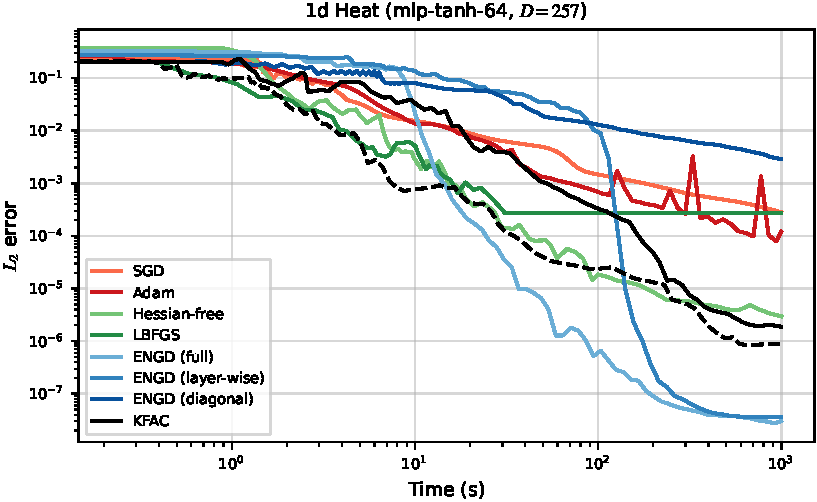
\includegraphics[trim={0 1.3cm 0 0},clip]{\pathToFigs/l2_error_over_time.pdf}
    % trim the legend and titles
    % [trim={left bottom right top},clip]
    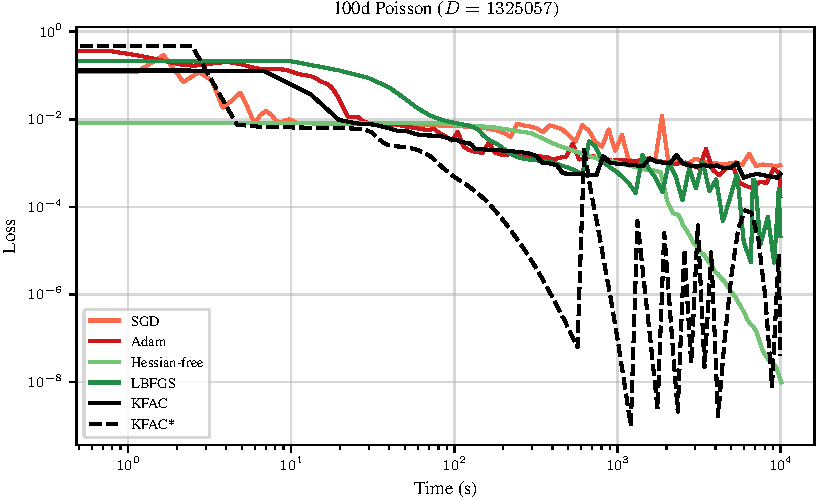
\includegraphics[trim={0 0.8cm 0 0.3cm},clip]{\pathToFigs/loss_over_time.pdf}
  \end{subfigure}
  \begin{subfigure}[t]{1.0\linewidth}
    \caption{}\label{subfig:poisson2d-step}
    % trim the legend, xlabel and xticklabels
    % [trim={left bottom right top},clip]
    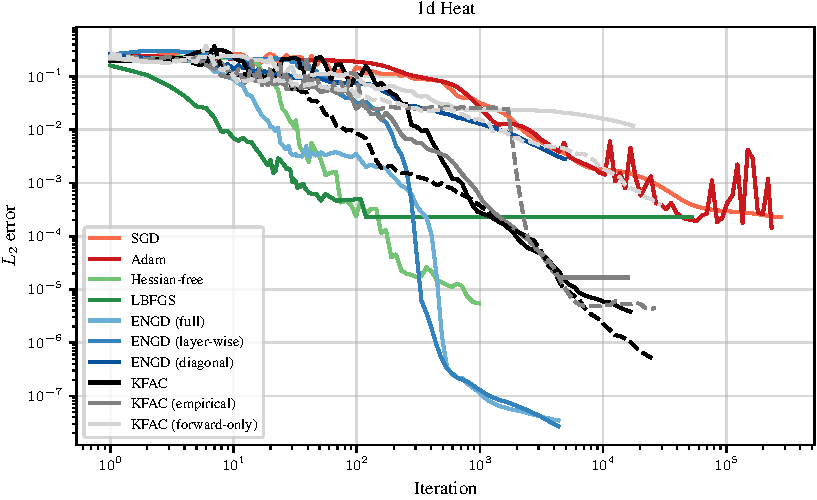
\includegraphics[trim={0 1.3cm 0 0.3cm},clip]{\pathToFigs/l2_error_over_step.pdf}
    % trim the titles
    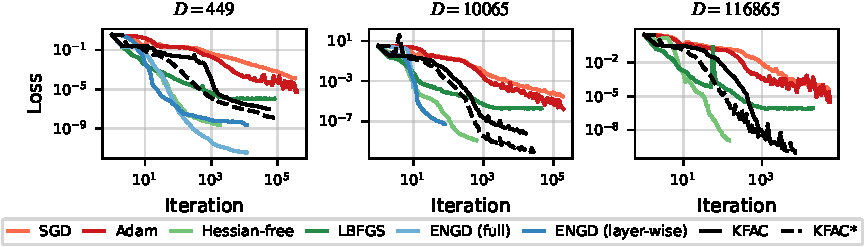
\includegraphics[trim={0 0 0 0.3cm},clip]{\pathToFigs/loss_over_step.pdf}
  \end{subfigure}
  \caption{ Training loss and evaluation $L_2$ error for learning the solution to a 2d Poisson equation over (\subref{subfig:poisson2d-time}) time and (\subref{subfig:poisson2d-step}) steps.
    Columns are different neural networks.}\label{fig:poisson2d-appendix}
\end{figure}

\begin{table}[!h]
  \centering
  \def\pathToRuns{kfac_pinns_exp/exp42_visualize_solutions/visualize_solution}
  \renewcommand\tabularxcolumn[1]{>{\Centering}m{#1}}
  \begin{small}
    \begin{tabularx}{\textwidth}{XXXXXX}
      \textbf{Optimizer} & \textbf{First step} & \textbf{0.1\% trained} & \textbf{1\% trained} & \textbf{10\% trained} & \textbf{True solution}
      \\
      SGD
      % [trim={left bottom right top},clip]
      &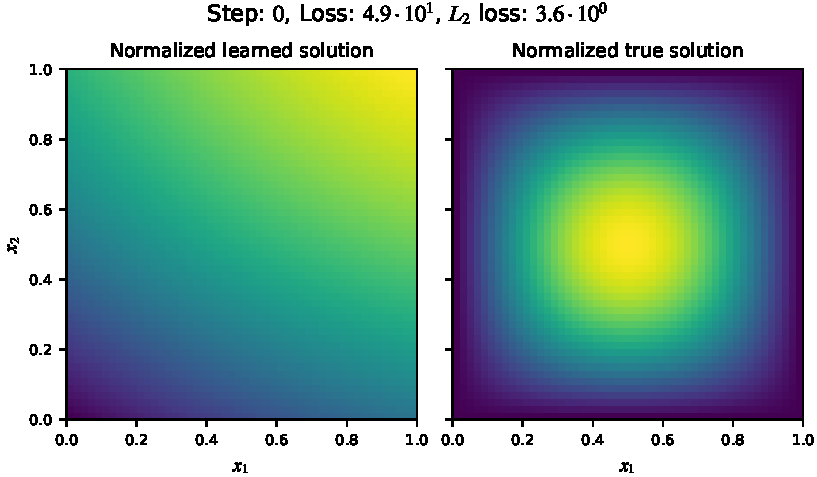
\includegraphics[trim={0.9cm 0.8cm 6.5cm 1.0cm},clip,scale=0.31]{\pathToRuns/SGD/poisson_2d_sin_product_mlp-tanh-64_SGD_step0000000.pdf}
      &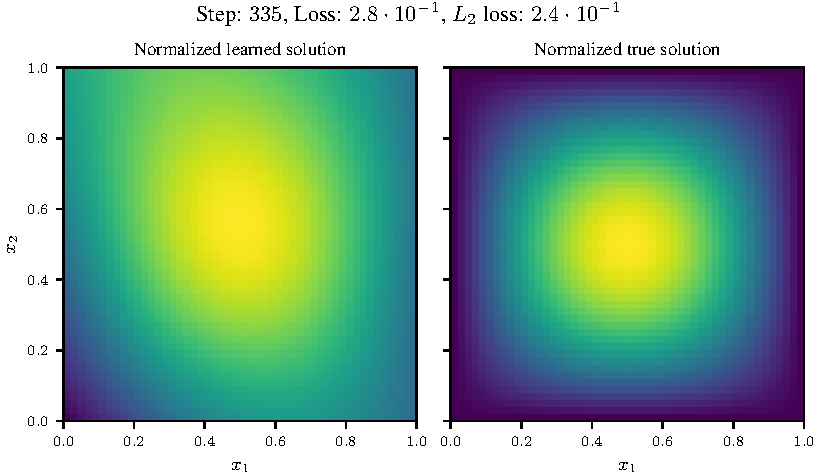
\includegraphics[trim={0.9cm 0.8cm 6.5cm 1.0cm},clip,scale=0.31]{\pathToRuns/SGD/poisson_2d_sin_product_mlp-tanh-64_SGD_step0000335.pdf}
      &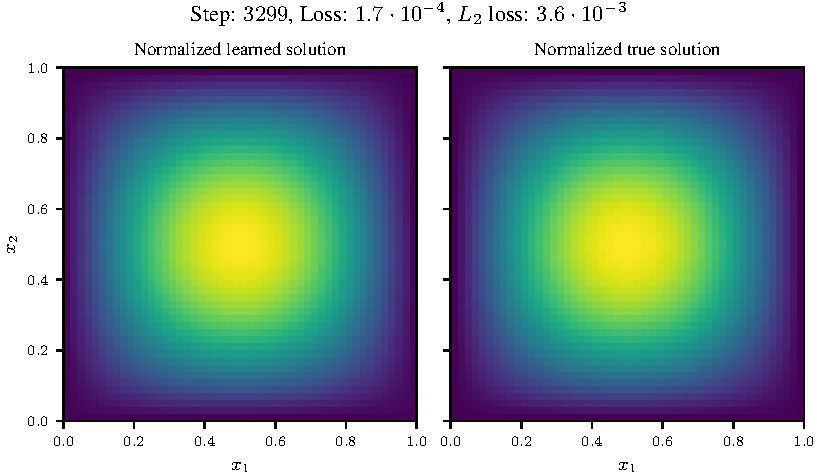
\includegraphics[trim={0.9cm 0.8cm 6.5cm 1.0cm},clip,scale=0.31]{\pathToRuns/SGD/poisson_2d_sin_product_mlp-tanh-64_SGD_step0003299.pdf}
      &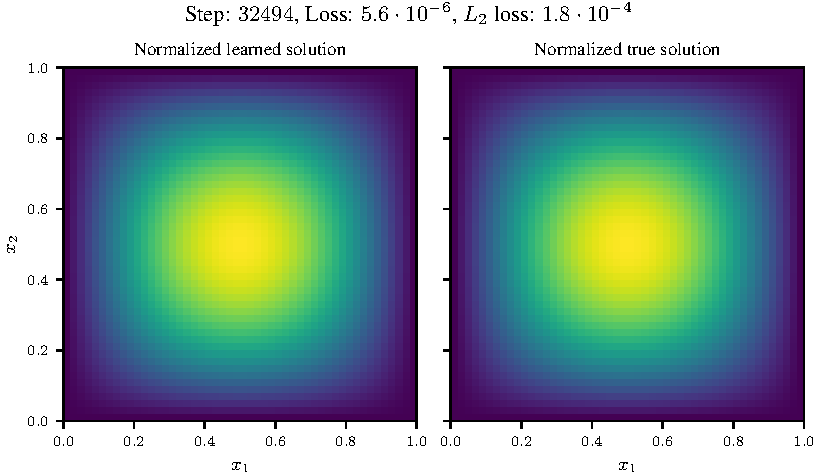
\includegraphics[trim={0.9cm 0.8cm 6.5cm 1.0cm},clip,scale=0.31]{\pathToRuns/SGD/poisson_2d_sin_product_mlp-tanh-64_SGD_step0032494.pdf}
      &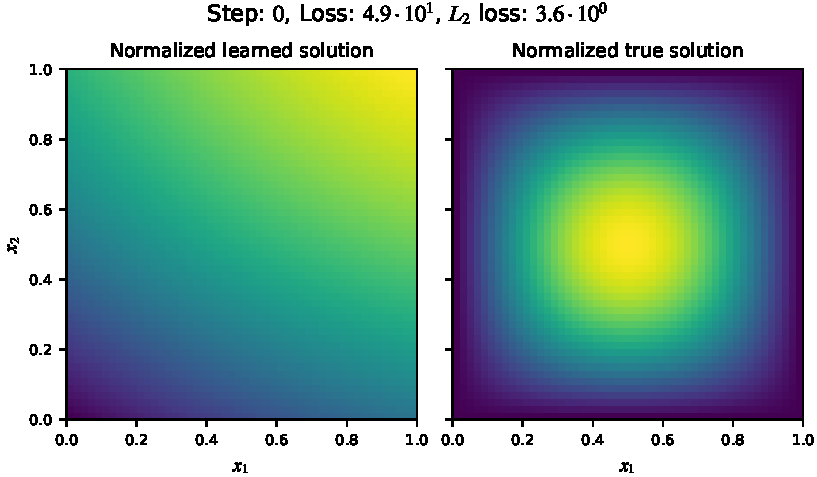
\includegraphics[trim={7.25cm 0.8cm 0 1.0cm},clip,scale=0.31]{\pathToRuns/SGD/poisson_2d_sin_product_mlp-tanh-64_SGD_step0000000.pdf}
      \\
      Adam
      % [trim={left bottom right top},clip]
      &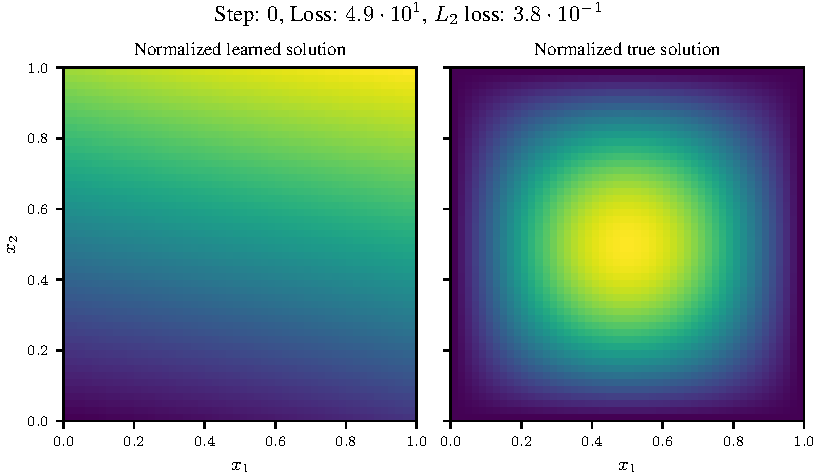
\includegraphics[trim={0.9cm 0.8cm 6.5cm 1.0cm},clip,scale=0.31]{\pathToRuns/Adam/poisson_2d_sin_product_mlp-tanh-64_Adam_step0000000.pdf}
      &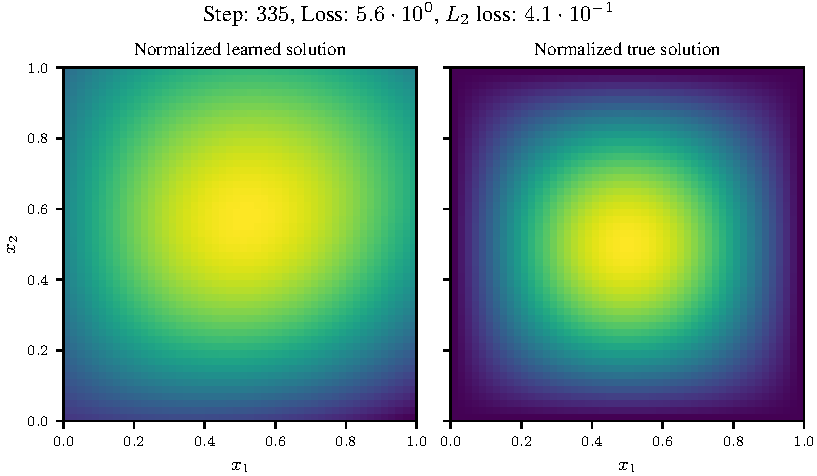
\includegraphics[trim={0.9cm 0.8cm 6.5cm 1.0cm},clip,scale=0.31]{\pathToRuns/Adam/poisson_2d_sin_product_mlp-tanh-64_Adam_step0000335.pdf}
      &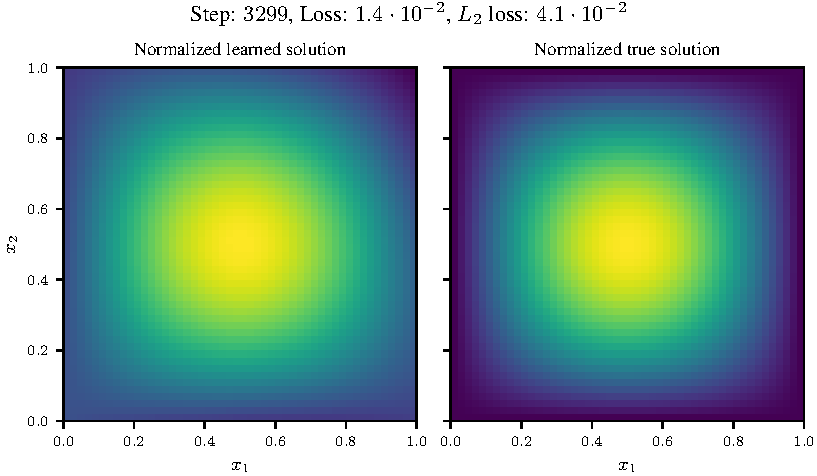
\includegraphics[trim={0.9cm 0.8cm 6.5cm 1.0cm},clip,scale=0.31]{\pathToRuns/Adam/poisson_2d_sin_product_mlp-tanh-64_Adam_step0003299.pdf}
      &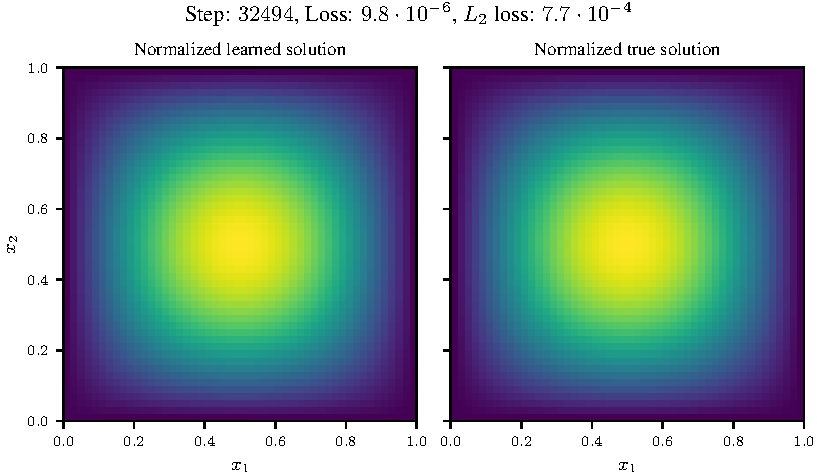
\includegraphics[trim={0.9cm 0.8cm 6.5cm 1.0cm},clip,scale=0.31]{\pathToRuns/Adam/poisson_2d_sin_product_mlp-tanh-64_Adam_step0032494.pdf}
      &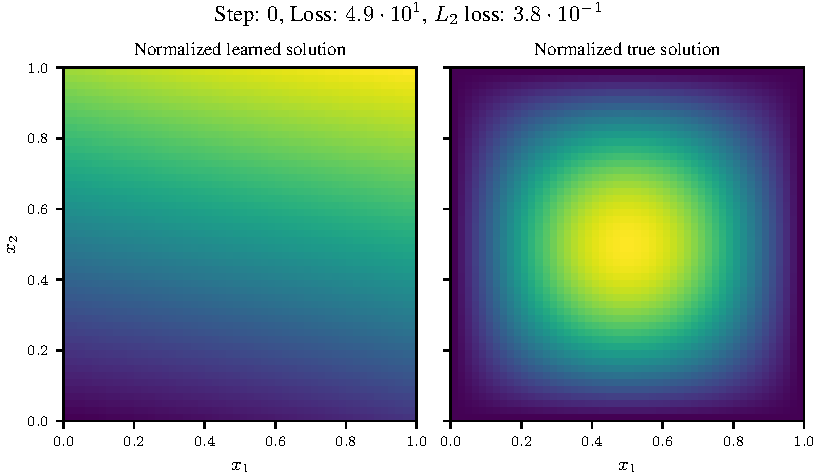
\includegraphics[trim={7.25cm 0.8cm 0 1.0cm},clip,scale=0.31]{\pathToRuns/Adam/poisson_2d_sin_product_mlp-tanh-64_Adam_step0000000.pdf}
      \\
      % [trim={left bottom right top},clip]
      LBFGS
      & 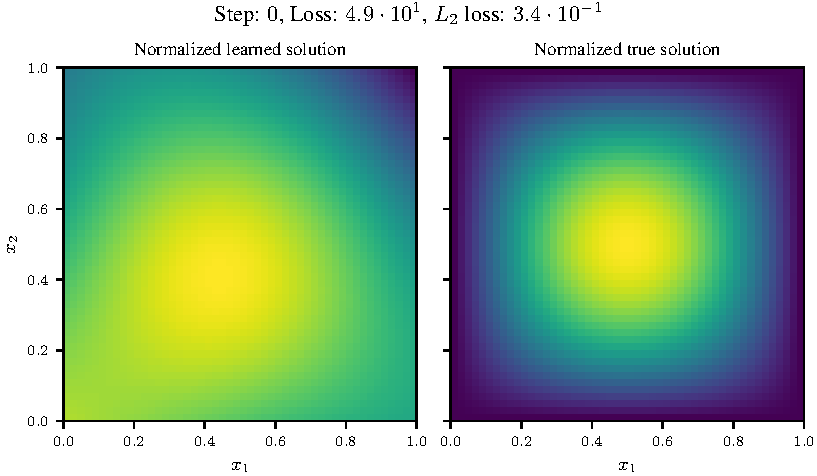
\includegraphics[trim={0.9cm 0.8cm 6.5cm 1.0cm},clip,scale=0.31]{\pathToRuns/LBFGS/poisson_2d_sin_product_mlp-tanh-64_LBFGS_step0000000.pdf}
      & 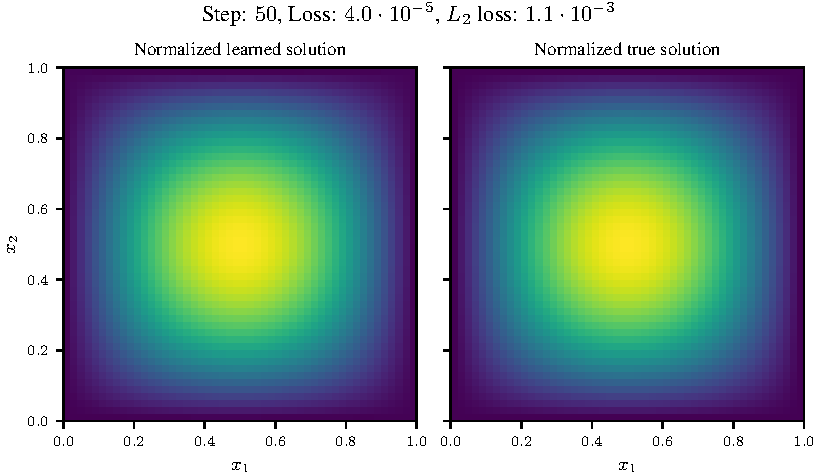
\includegraphics[trim={0.9cm 0.8cm 6.5cm 1.0cm},clip,scale=0.31]{\pathToRuns/LBFGS/poisson_2d_sin_product_mlp-tanh-64_LBFGS_step0000050.pdf}
      & 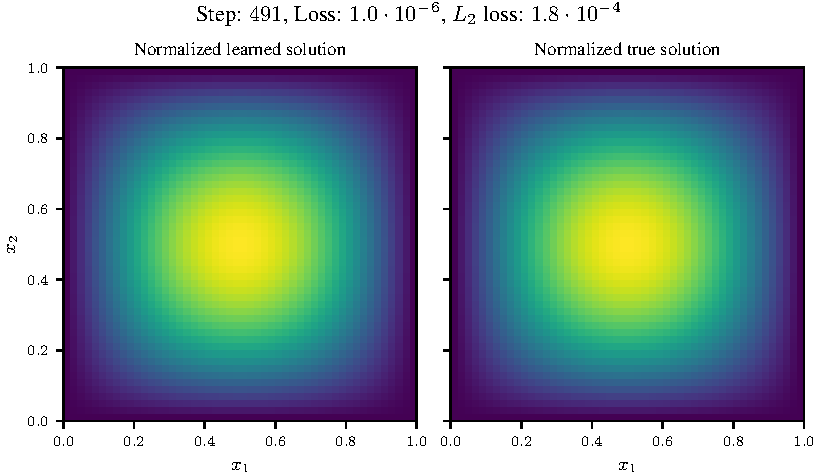
\includegraphics[trim={0.9cm 0.8cm 6.5cm 1.0cm},clip,scale=0.31]{\pathToRuns/LBFGS/poisson_2d_sin_product_mlp-tanh-64_LBFGS_step0000491.pdf}
      & 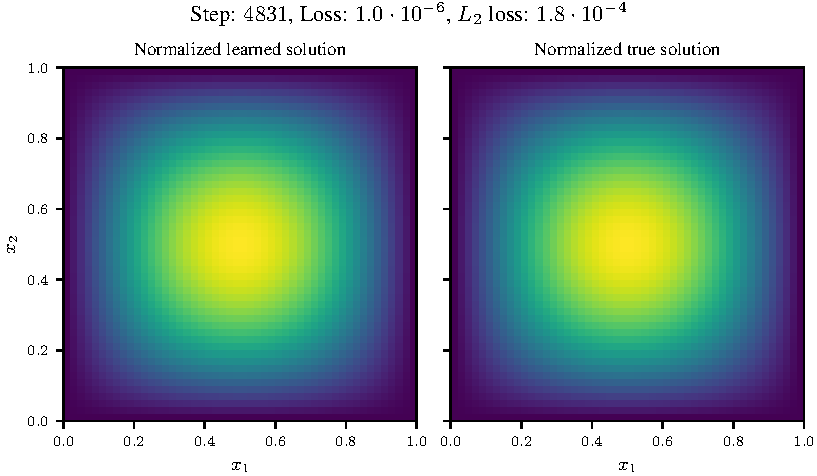
\includegraphics[trim={0.9cm 0.8cm 6.5cm 1.0cm},clip,scale=0.31]{\pathToRuns/LBFGS/poisson_2d_sin_product_mlp-tanh-64_LBFGS_step0004831.pdf}
      & 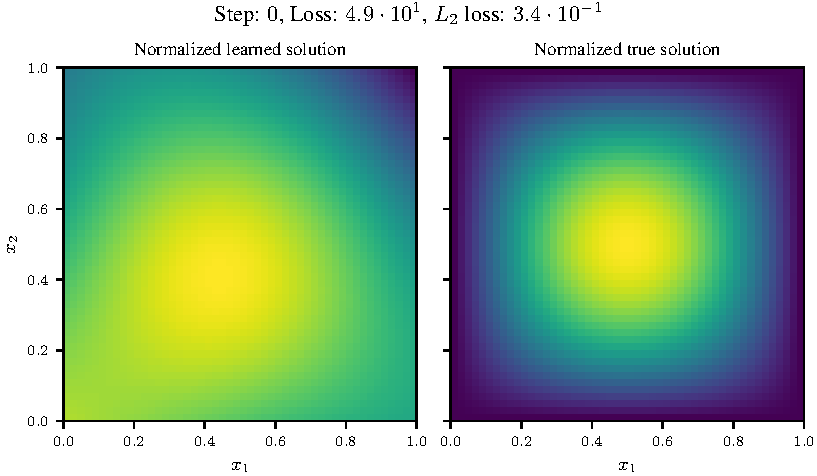
\includegraphics[trim={7.25cm 0.8cm 0 1.0cm},clip,scale=0.31]{\pathToRuns/LBFGS/poisson_2d_sin_product_mlp-tanh-64_LBFGS_step0000000.pdf}
      \\
      Hessian-free
      % [trim={left bottom right top},clip]
      &\includegraphics[trim={0.9cm 0.8cm 6.5cm 1.0cm},clip,scale=0.31]{\pathToRuns/Hessian-free/poisson_2d_sin_product_mlp-tanh-64_Hessianfree_step0000000.pdf}
      &\includegraphics[trim={0.9cm 0.8cm 6.5cm 1.0cm},clip,scale=0.31]{\pathToRuns/Hessian-free/poisson_2d_sin_product_mlp-tanh-64_Hessianfree_step0000004.pdf}
      &\includegraphics[trim={0.9cm 0.8cm 6.5cm 1.0cm},clip,scale=0.31]{\pathToRuns/Hessian-free/poisson_2d_sin_product_mlp-tanh-64_Hessianfree_step0000035.pdf}
      &\includegraphics[trim={0.9cm 0.8cm 6.5cm 1.0cm},clip,scale=0.31]{\pathToRuns/Hessian-free/poisson_2d_sin_product_mlp-tanh-64_Hessianfree_step0000335.pdf}
      &\includegraphics[trim={7.25cm 0.8cm 0 1.0cm},clip,scale=0.31]{\pathToRuns/Hessian-free/poisson_2d_sin_product_mlp-tanh-64_Hessianfree_step0000000.pdf}
      \\
      % [trim={left bottom right top},clip]
      ENGD (full)
      &\includegraphics[trim={0.9cm 0.8cm 6.5cm 1.0cm},clip,scale=0.31]{\pathToRuns/ENGD_full/poisson_2d_sin_product_mlp-tanh-64_ENGD_step0000000.pdf}
      &\includegraphics[trim={0.9cm 0.8cm 6.5cm 1.0cm},clip,scale=0.31]{\pathToRuns/ENGD_full/poisson_2d_sin_product_mlp-tanh-64_ENGD_step0000006.pdf}
      &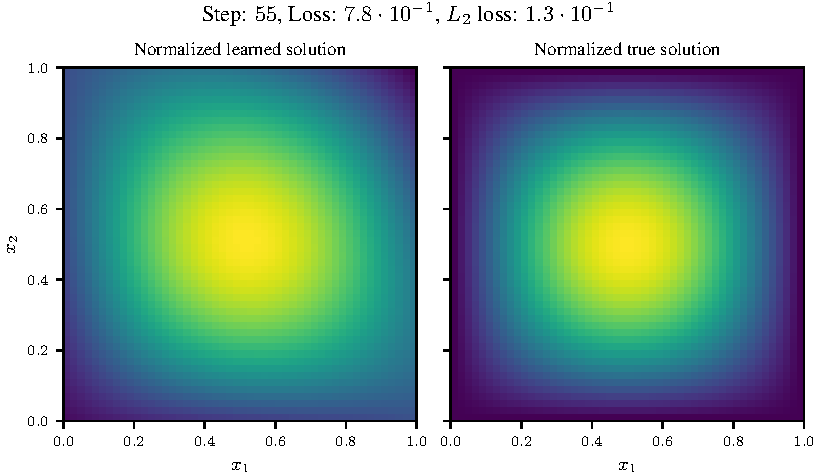
\includegraphics[trim={0.9cm 0.8cm 6.5cm 1.0cm},clip,scale=0.31]{\pathToRuns/ENGD_full/poisson_2d_sin_product_mlp-tanh-64_ENGD_step0000055.pdf}
      &\includegraphics[trim={0.9cm 0.8cm 6.5cm 1.0cm},clip,scale=0.31]{\pathToRuns/ENGD_full/poisson_2d_sin_product_mlp-tanh-64_ENGD_step0000594.pdf}
      &\includegraphics[trim={7.25cm 0.8cm 0 1.0cm},clip,scale=0.31]{\pathToRuns/ENGD_full/poisson_2d_sin_product_mlp-tanh-64_ENGD_step0000000.pdf}
      \\
      ENGD (layer-wise)
      % [trim={left bottom right top},clip]
      &\includegraphics[trim={0.9cm 0.8cm 6.5cm 1.0cm},clip,scale=0.31]{\pathToRuns/ENGD_layer-wise/poisson_2d_sin_product_mlp-tanh-64_ENGD_step0000000.pdf}
      &\includegraphics[trim={0.9cm 0.8cm 6.5cm 1.0cm},clip,scale=0.31]{\pathToRuns/ENGD_layer-wise/poisson_2d_sin_product_mlp-tanh-64_ENGD_step0000006.pdf}
      &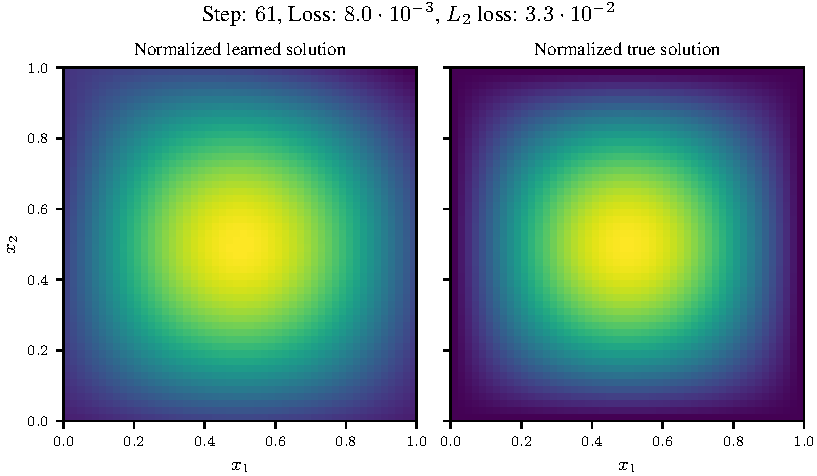
\includegraphics[trim={0.9cm 0.8cm 6.5cm 1.0cm},clip,scale=0.31]{\pathToRuns/ENGD_layer-wise/poisson_2d_sin_product_mlp-tanh-64_ENGD_step0000061.pdf}
      &\includegraphics[trim={0.9cm 0.8cm 6.5cm 1.0cm},clip,scale=0.31]{\pathToRuns/ENGD_layer-wise/poisson_2d_sin_product_mlp-tanh-64_ENGD_step0000594.pdf}
      &\includegraphics[trim={7.25cm 0.8cm 0 1.0cm},clip,scale=0.31]{\pathToRuns/ENGD_layer-wise/poisson_2d_sin_product_mlp-tanh-64_ENGD_step0000000.pdf}
      \\
      KFAC
      % [trim={left bottom right top},clip]
      &\includegraphics[trim={0.9cm 0.8cm 6.5cm 1.0cm},clip,scale=0.31]{\pathToRuns/KFAC/poisson_2d_sin_product_mlp-tanh-64_KFAC_step0000000.pdf}
      &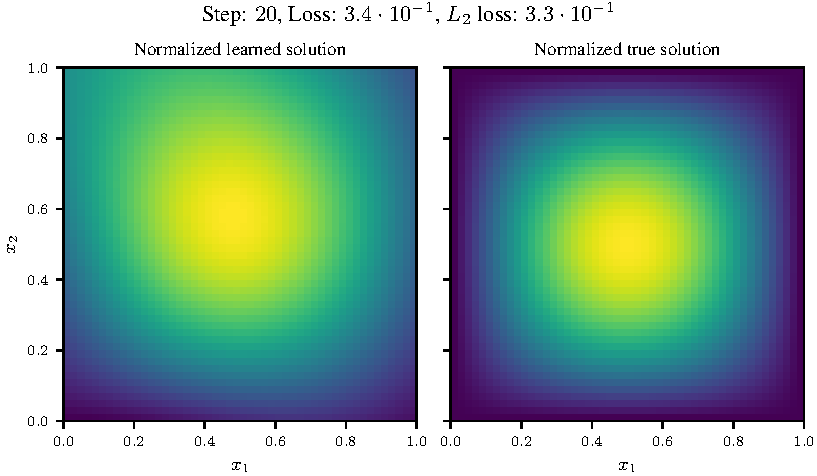
\includegraphics[trim={0.9cm 0.8cm 6.5cm 1.0cm},clip,scale=0.31]{\pathToRuns/KFAC/poisson_2d_sin_product_mlp-tanh-64_KFAC_step0000020.pdf}
      &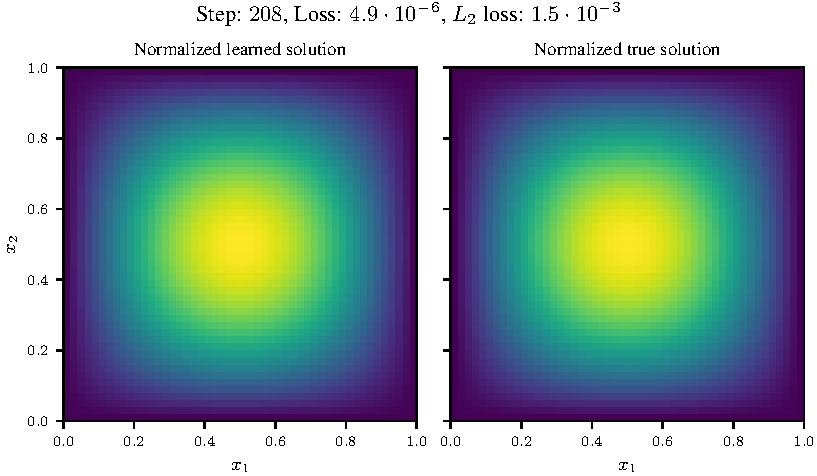
\includegraphics[trim={0.9cm 0.8cm 6.5cm 1.0cm},clip,scale=0.31]{\pathToRuns/KFAC/poisson_2d_sin_product_mlp-tanh-64_KFAC_step0000208.pdf}
      &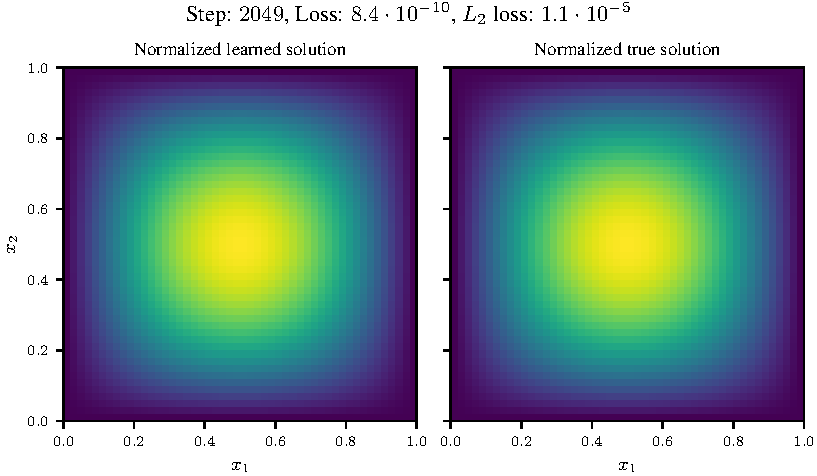
\includegraphics[trim={0.9cm 0.8cm 6.5cm 1.0cm},clip,scale=0.31]{\pathToRuns/KFAC/poisson_2d_sin_product_mlp-tanh-64_KFAC_step0002049.pdf}
      &\includegraphics[trim={7.25cm 0.8cm 0 1.0cm},clip,scale=0.31]{\pathToRuns/KFAC/poisson_2d_sin_product_mlp-tanh-64_KFAC_step0000000.pdf}
      \\
      KFAC*
      % [trim={left bottom right top},clip]
      &\includegraphics[trim={0.9cm 0.8cm 6.5cm 1.0cm},clip,scale=0.31]{\pathToRuns/KFAC_auto/poisson_2d_sin_product_mlp-tanh-64_KFAC_step0000000.pdf}
      &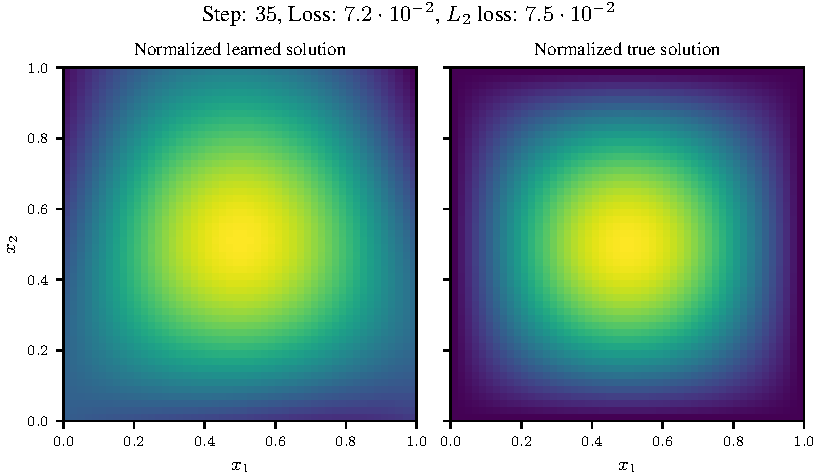
\includegraphics[trim={0.9cm 0.8cm 6.5cm 1.0cm},clip,scale=0.31]{\pathToRuns/KFAC_auto/poisson_2d_sin_product_mlp-tanh-64_KFAC_step0000035.pdf}
      &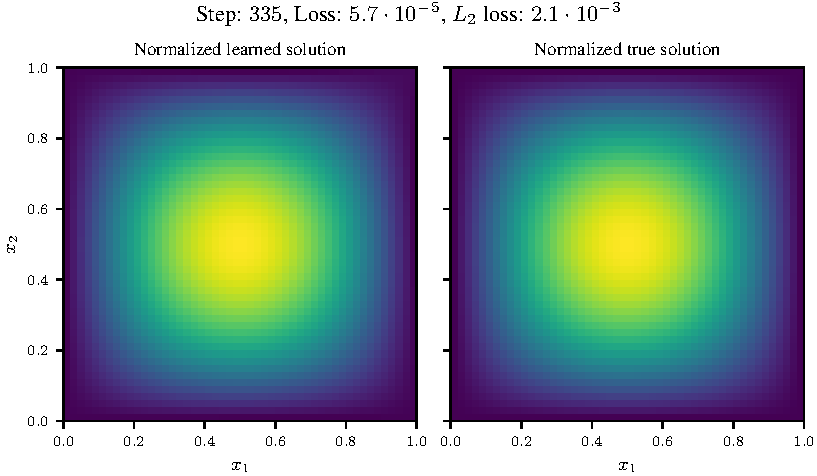
\includegraphics[trim={0.9cm 0.8cm 6.5cm 1.0cm},clip,scale=0.31]{\pathToRuns/KFAC_auto/poisson_2d_sin_product_mlp-tanh-64_KFAC_step0000335.pdf}
      &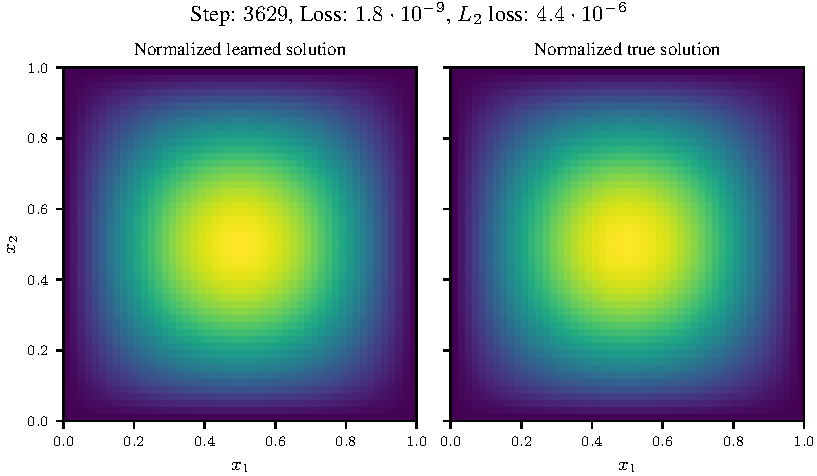
\includegraphics[trim={0.9cm 0.8cm 6.5cm 1.0cm},clip,scale=0.31]{\pathToRuns/KFAC_auto/poisson_2d_sin_product_mlp-tanh-64_KFAC_step0003629.pdf}
      &\includegraphics[trim={7.25cm 0.8cm 0 1.0cm},clip,scale=0.31]{\pathToRuns/KFAC_auto/poisson_2d_sin_product_mlp-tanh-64_KFAC_step0000000.pdf}
    \end{tabularx}
  \end{small}
  \captionof{figure}{Visual comparison learned and true solutions while training with different optimizers for the 2d Poisson equation using a two-layer MLP (corresponding to the curves in \Cref{fig:2D-Poisson} left).
    All functions are shown on the unit square $(x, y) \in \Omega = [0; 1]^2$ and normalized to the unit interval.}
  \label{fig:2d-poisson-visualization}
\end{table}

\paragraph{Best run details}
The runs shown in \Cref{fig:poisson2d-appendix} correspond to the following hyper-parameters:
\begin{itemize}
\item $2\to 64\to 1$ MLP with $D=257$
  \begin{itemize}
    \def\pathToRuns{kfac_pinns_exp/exp09_reproduce_poisson2d/tex}
  \item \textbf{SGD:} learning rate: $\num[scientific-notation=true]{1.007555e-03}$, momentum: $\num[scientific-notation=true]{0.9}$
  \item \textbf{Adam:} learning rate: $\num[scientific-notation=true]{1.369294e-06}$, $N_{\Omega}$: $\num[scientific-notation=false]{203}$, $N_{\partial\Omega}$: $\num[scientific-notation=false]{1494}$, batch sampling frequency: $\num[scientific-notation=false]{9712}$
  \item \textbf{Hessian-free:} curvature matrix: $\text{GGN}$, initial damping: $\num[scientific-notation=true]{1.146081e-02}$, constant damping: $\text{no}$, maximum CG iterations: $\num[scientific-notation=false]{484}$, $N_{\Omega}$: $\num[scientific-notation=false]{2410}$, $N_{\partial\Omega}$: $\num[scientific-notation=false]{2448}$, batch sampling frequency: $\num[scientific-notation=false]{1311}$
  \item \textbf{LBFGS:} learning rate: $\num[scientific-notation=true]{0.2}$, history size: $\num[scientific-notation=false]{225}$
  \item \textbf{ENGD (full):} damping: $\num[scientific-notation=true]{1e-10}$, exponential moving average: $\num[scientific-notation=true]{0.3}$, initialize Gramian to identity: $\text{yes}$
  \item \textbf{ENGD (layer-wise):} damping: $\num[scientific-notation=true]{1e-06}$, exponential moving average: $\num[scientific-notation=true]{0.3}$, initialize Gramian to identity: $\text{no}$
  \item \textbf{KFAC:} damping: $\num[scientific-notation=true]{8.435180e-14}$, momentum: $\num[scientific-notation=true]{9.718645e-01}$, exponential moving average: $\num[scientific-notation=true]{9.800744e-01}$, initialize Kronecker factors to identity: $\text{yes}$, $N_{\Omega}$: $\num[scientific-notation=false]{2525}$, $N_{\partial\Omega}$: $\num[scientific-notation=false]{2663}$, batch sampling frequency: $\num[scientific-notation=false]{7916}$
  \item \textbf{KFAC*:} damping: $\num[scientific-notation=true]{2.965060e-08}$, exponential moving average: $\num[scientific-notation=true]{9.574717e-01}$, initialize Kronecker factors to identity: $\text{yes}$
  \end{itemize}

\item $2 \to 64 \to 64 \to 48 \to 48 \to 1$ MLP with $D=\num{9873}$
  \begin{itemize}
    \def\pathToRuns{kfac_pinns_exp/exp15_poisson2d_deepwide/tex}
  \item \textbf{SGD:} learning rate: $\num[scientific-notation=true]{1.007555e-03}$, momentum: $\num[scientific-notation=true]{0.9}$
  \item \textbf{Adam:} learning rate: $\num[scientific-notation=true]{1.369294e-06}$, $N_{\Omega}$: $\num[scientific-notation=false]{203}$, $N_{\partial\Omega}$: $\num[scientific-notation=false]{1494}$, batch sampling frequency: $\num[scientific-notation=false]{9712}$
  \item \textbf{Hessian-free:} curvature matrix: $\text{GGN}$, initial damping: $\num[scientific-notation=true]{1.146081e-02}$, constant damping: $\text{no}$, maximum CG iterations: $\num[scientific-notation=false]{484}$, $N_{\Omega}$: $\num[scientific-notation=false]{2410}$, $N_{\partial\Omega}$: $\num[scientific-notation=false]{2448}$, batch sampling frequency: $\num[scientific-notation=false]{1311}$
  \item \textbf{LBFGS:} learning rate: $\num[scientific-notation=true]{0.2}$, history size: $\num[scientific-notation=false]{225}$
  \item \textbf{ENGD (full):} damping: $\num[scientific-notation=true]{1e-10}$, exponential moving average: $\num[scientific-notation=true]{0.3}$, initialize Gramian to identity: $\text{yes}$
  \item \textbf{ENGD (layer-wise):} damping: $\num[scientific-notation=true]{1e-06}$, exponential moving average: $\num[scientific-notation=true]{0.3}$, initialize Gramian to identity: $\text{no}$
  \item \textbf{KFAC:} damping: $\num[scientific-notation=true]{8.435180e-14}$, momentum: $\num[scientific-notation=true]{9.718645e-01}$, exponential moving average: $\num[scientific-notation=true]{9.800744e-01}$, initialize Kronecker factors to identity: $\text{yes}$, $N_{\Omega}$: $\num[scientific-notation=false]{2525}$, $N_{\partial\Omega}$: $\num[scientific-notation=false]{2663}$, batch sampling frequency: $\num[scientific-notation=false]{7916}$
  \item \textbf{KFAC*:} damping: $\num[scientific-notation=true]{2.965060e-08}$, exponential moving average: $\num[scientific-notation=true]{9.574717e-01}$, initialize Kronecker factors to identity: $\text{yes}$
  \end{itemize}

\item $2 \to 256 \to 256\to 128 \to 128 \to 1$ MLP with $D=\num{116097}$
  \begin{itemize}
    \def\pathToRuns{kfac_pinns_exp/exp20_poisson2d_mlp_tanh_256/tex}
  \item \textbf{SGD:} learning rate: $\num[scientific-notation=true]{1.007555e-03}$, momentum: $\num[scientific-notation=true]{0.9}$
  \item \textbf{Adam:} learning rate: $\num[scientific-notation=true]{1.369294e-06}$, $N_{\Omega}$: $\num[scientific-notation=false]{203}$, $N_{\partial\Omega}$: $\num[scientific-notation=false]{1494}$, batch sampling frequency: $\num[scientific-notation=false]{9712}$
  \item \textbf{Hessian-free:} curvature matrix: $\text{GGN}$, initial damping: $\num[scientific-notation=true]{1.146081e-02}$, constant damping: $\text{no}$, maximum CG iterations: $\num[scientific-notation=false]{484}$, $N_{\Omega}$: $\num[scientific-notation=false]{2410}$, $N_{\partial\Omega}$: $\num[scientific-notation=false]{2448}$, batch sampling frequency: $\num[scientific-notation=false]{1311}$
  \item \textbf{LBFGS:} learning rate: $\num[scientific-notation=true]{0.2}$, history size: $\num[scientific-notation=false]{225}$
  \item \textbf{KFAC:} damping: $\num[scientific-notation=true]{8.435180e-14}$, momentum: $\num[scientific-notation=true]{9.718645e-01}$, exponential moving average: $\num[scientific-notation=true]{9.800744e-01}$, initialize Kronecker factors to identity: $\text{yes}$, $N_{\Omega}$: $\num[scientific-notation=false]{2525}$, $N_{\partial\Omega}$: $\num[scientific-notation=false]{2663}$, batch sampling frequency: $\num[scientific-notation=false]{7916}$
  \item \textbf{KFAC*:} damping: $\num[scientific-notation=true]{2.965060e-08}$, exponential moving average: $\num[scientific-notation=true]{9.574717e-01}$, initialize Kronecker factors to identity: $\text{yes}$
  \end{itemize}
\end{itemize}

\paragraph{Search space details} The runs shown in \Cref{fig:poisson2d-appendix} were determined to be the best via a search with approximately 50 runs on the following search spaces which were obtained by refining an initially wider search ($\mathcal{U}$ denotes a uniform, and $\mathcal{LU}$ a log-uniform distribution):
\begin{itemize}
\item $2\to 64\to 1$ MLP with $D=257$
  \begin{itemize}
    \def\pathToRuns{kfac_pinns_exp/exp09_reproduce_poisson2d/tex}
  \item \textbf{SGD:} learning rate: $\mathcal{LU}([\num[scientific-notation=true]{1e-06}; \num[scientific-notation=false]{1}])$, momentum: $\mathcal{U}([\num[scientific-notation=false]{0}; \num[scientific-notation=true]{0.99}])$, $N_{\Omega}$: $\mathcal{C}(\{\num[scientific-notation=false]{100},\num[scientific-notation=false]{101},\text{\dots},\num[scientific-notation=false]{5000}\})$, $N_{\partial\Omega}$: $\mathcal{C}(\{\num[scientific-notation=false]{50},\num[scientific-notation=false]{51},\text{\dots},\num[scientific-notation=false]{2500}\})$, batch sampling frequency: $\mathcal{C}(\{\num[scientific-notation=false]{0},\num[scientific-notation=false]{1},\text{\dots},\num[scientific-notation=false]{1000}\})$
  \item \textbf{Adam:} learning rate: $\mathcal{LU}([\num[scientific-notation=true]{0.0001}; \num[scientific-notation=true]{0.5}])$
  \item \textbf{Hessian-free:} curvature matrix: $\mathcal{U}(\{\text{GGN},\text{Hessian}\})$, initial damping: $\mathcal{LU}([\num[scientific-notation=true]{1e-15}; \num[scientific-notation=false]{1}])$, constant damping: $\mathcal{U}(\{\text{no},\text{yes}\})$, maximum CG iterations: $\mathcal{U}(\{\num[scientific-notation=false]{1},\num[scientific-notation=false]{2},\text{\dots},\num[scientific-notation=false]{500}\})$, $N_{\Omega}$: $\mathcal{U}(\{\num[scientific-notation=false]{100},\num[scientific-notation=false]{101},\text{\dots},\num[scientific-notation=false]{5000}\})$, $N_{\partial\Omega}$: $\mathcal{U}(\{\num[scientific-notation=false]{50},\num[scientific-notation=false]{51},\text{\dots},\num[scientific-notation=false]{2500}\})$, batch sampling frequency: $\mathcal{U}(\{\num[scientific-notation=false]{0},\num[scientific-notation=false]{1},\text{\dots},\num[scientific-notation=false]{5000}\})$
  \item \textbf{LBFGS:} learning rate: $\mathcal{C}(\{\num[scientific-notation=true]{0.5},\num[scientific-notation=true]{0.2},\num[scientific-notation=true]{0.1},\num[scientific-notation=true]{0.05},\num[scientific-notation=true]{0.02},\num[scientific-notation=true]{0.01}\})$, history size: $\mathcal{C}(\{\num[scientific-notation=false]{75},\num[scientific-notation=false]{100},\num[scientific-notation=false]{125},\num[scientific-notation=false]{150},\num[scientific-notation=false]{175},\num[scientific-notation=false]{200},\num[scientific-notation=false]{225},\num[scientific-notation=false]{250}\})$
  \item \textbf{ENGD (full):} damping: $\mathcal{C}(\{\num[scientific-notation=true]{1e-08},\num[scientific-notation=true]{1e-09},\num[scientific-notation=true]{1e-10},\num[scientific-notation=true]{1e-11},\num[scientific-notation=true]{1e-12},\num[scientific-notation=false]{0}\})$, exponential moving average: $\mathcal{C}(\{\num[scientific-notation=false]{0},\num[scientific-notation=true]{0.3},\num[scientific-notation=true]{0.6},\num[scientific-notation=true]{0.9}\})$, initialize Gramian to identity: $\mathcal{C}(\{\text{no},\text{yes}\})$
  \item \textbf{ENGD (layer-wise):} damping: $\mathcal{U}(\{\num[scientific-notation=true]{0.01},\num[scientific-notation=true]{0.001},\num[scientific-notation=true]{0.0001},\num[scientific-notation=true]{1e-05},\num[scientific-notation=true]{1e-06}\})$, exponential moving average: $\mathcal{U}(\{\num[scientific-notation=false]{0},\num[scientific-notation=true]{0.3},\num[scientific-notation=true]{0.6},\num[scientific-notation=true]{0.9},\num[scientific-notation=true]{0.99}\})$, initialize Gramian to identity: $\mathcal{U}(\{\text{no},\text{yes}\})$
  \item \textbf{KFAC:} damping: $\mathcal{LU}([\num[scientific-notation=true]{1e-15}; \num[scientific-notation=true]{0.01}])$, momentum: $\mathcal{U}([\num[scientific-notation=false]{0}; \num[scientific-notation=true]{0.99}])$, exponential moving average: $\mathcal{U}([\num[scientific-notation=false]{0}; \num[scientific-notation=true]{0.99}])$, initialize Kronecker factors to identity: $\mathcal{C}(\{\text{no},\text{yes}\})$
  \item \textbf{KFAC*:} damping: $\mathcal{LU}([\num[scientific-notation=true]{1e-15}; \num[scientific-notation=true]{0.01}])$, exponential moving average: $\mathcal{U}([\num[scientific-notation=false]{0}; \num[scientific-notation=true]{0.99}])$, initialize Kronecker factors to identity: $\mathcal{U}(\{\text{no},\text{yes}\})$, $N_{\Omega}$: $\mathcal{U}(\{\num[scientific-notation=false]{100},\num[scientific-notation=false]{101},\text{\dots},\num[scientific-notation=false]{5000}\})$, $N_{\partial\Omega}$: $\mathcal{U}(\{\num[scientific-notation=false]{50},\num[scientific-notation=false]{51},\text{\dots},\num[scientific-notation=false]{2500}\})$, batch sampling frequency: $\mathcal{U}(\{\num[scientific-notation=false]{0},\num[scientific-notation=false]{1},\text{\dots},\num[scientific-notation=false]{5000}\})$
  \end{itemize}

\item $2 \to 64 \to 64 \to 48 \to 48 \to 1$ MLP with $D=\num{9873}$
  \begin{itemize}
    \def\pathToRuns{kfac_pinns_exp/exp15_poisson2d_deepwide/tex}
  \item \textbf{SGD:} learning rate: $\mathcal{LU}([\num[scientific-notation=true]{1e-06}; \num[scientific-notation=false]{1}])$, momentum: $\mathcal{U}([\num[scientific-notation=false]{0}; \num[scientific-notation=true]{0.99}])$, $N_{\Omega}$: $\mathcal{C}(\{\num[scientific-notation=false]{100},\num[scientific-notation=false]{101},\text{\dots},\num[scientific-notation=false]{5000}\})$, $N_{\partial\Omega}$: $\mathcal{C}(\{\num[scientific-notation=false]{50},\num[scientific-notation=false]{51},\text{\dots},\num[scientific-notation=false]{2500}\})$, batch sampling frequency: $\mathcal{C}(\{\num[scientific-notation=false]{0},\num[scientific-notation=false]{1},\text{\dots},\num[scientific-notation=false]{1000}\})$
  \item \textbf{Adam:} learning rate: $\mathcal{LU}([\num[scientific-notation=true]{0.0001}; \num[scientific-notation=true]{0.5}])$
  \item \textbf{Hessian-free:} curvature matrix: $\mathcal{U}(\{\text{GGN},\text{Hessian}\})$, initial damping: $\mathcal{LU}([\num[scientific-notation=true]{1e-15}; \num[scientific-notation=false]{1}])$, constant damping: $\mathcal{U}(\{\text{no},\text{yes}\})$, maximum CG iterations: $\mathcal{U}(\{\num[scientific-notation=false]{1},\num[scientific-notation=false]{2},\text{\dots},\num[scientific-notation=false]{500}\})$, $N_{\Omega}$: $\mathcal{U}(\{\num[scientific-notation=false]{100},\num[scientific-notation=false]{101},\text{\dots},\num[scientific-notation=false]{5000}\})$, $N_{\partial\Omega}$: $\mathcal{U}(\{\num[scientific-notation=false]{50},\num[scientific-notation=false]{51},\text{\dots},\num[scientific-notation=false]{2500}\})$, batch sampling frequency: $\mathcal{U}(\{\num[scientific-notation=false]{0},\num[scientific-notation=false]{1},\text{\dots},\num[scientific-notation=false]{5000}\})$
  \item \textbf{LBFGS:} learning rate: $\mathcal{C}(\{\num[scientific-notation=true]{0.5},\num[scientific-notation=true]{0.2},\num[scientific-notation=true]{0.1},\num[scientific-notation=true]{0.05},\num[scientific-notation=true]{0.02},\num[scientific-notation=true]{0.01}\})$, history size: $\mathcal{C}(\{\num[scientific-notation=false]{75},\num[scientific-notation=false]{100},\num[scientific-notation=false]{125},\num[scientific-notation=false]{150},\num[scientific-notation=false]{175},\num[scientific-notation=false]{200},\num[scientific-notation=false]{225},\num[scientific-notation=false]{250}\})$
  \item \textbf{ENGD (full):} damping: $\mathcal{C}(\{\num[scientific-notation=true]{1e-08},\num[scientific-notation=true]{1e-09},\num[scientific-notation=true]{1e-10},\num[scientific-notation=true]{1e-11},\num[scientific-notation=true]{1e-12},\num[scientific-notation=false]{0}\})$, exponential moving average: $\mathcal{C}(\{\num[scientific-notation=false]{0},\num[scientific-notation=true]{0.3},\num[scientific-notation=true]{0.6},\num[scientific-notation=true]{0.9}\})$, initialize Gramian to identity: $\mathcal{C}(\{\text{no},\text{yes}\})$
  \item \textbf{ENGD (layer-wise):} damping: $\mathcal{U}(\{\num[scientific-notation=true]{0.01},\num[scientific-notation=true]{0.001},\num[scientific-notation=true]{0.0001},\num[scientific-notation=true]{1e-05},\num[scientific-notation=true]{1e-06}\})$, exponential moving average: $\mathcal{U}(\{\num[scientific-notation=false]{0},\num[scientific-notation=true]{0.3},\num[scientific-notation=true]{0.6},\num[scientific-notation=true]{0.9},\num[scientific-notation=true]{0.99}\})$, initialize Gramian to identity: $\mathcal{U}(\{\text{no},\text{yes}\})$
  \item \textbf{KFAC:} damping: $\mathcal{LU}([\num[scientific-notation=true]{1e-15}; \num[scientific-notation=true]{0.01}])$, momentum: $\mathcal{U}([\num[scientific-notation=false]{0}; \num[scientific-notation=true]{0.99}])$, exponential moving average: $\mathcal{U}([\num[scientific-notation=false]{0}; \num[scientific-notation=true]{0.99}])$, initialize Kronecker factors to identity: $\mathcal{C}(\{\text{no},\text{yes}\})$
  \item \textbf{KFAC*:} damping: $\mathcal{LU}([\num[scientific-notation=true]{1e-15}; \num[scientific-notation=true]{0.01}])$, exponential moving average: $\mathcal{U}([\num[scientific-notation=false]{0}; \num[scientific-notation=true]{0.99}])$, initialize Kronecker factors to identity: $\mathcal{U}(\{\text{no},\text{yes}\})$, $N_{\Omega}$: $\mathcal{U}(\{\num[scientific-notation=false]{100},\num[scientific-notation=false]{101},\text{\dots},\num[scientific-notation=false]{5000}\})$, $N_{\partial\Omega}$: $\mathcal{U}(\{\num[scientific-notation=false]{50},\num[scientific-notation=false]{51},\text{\dots},\num[scientific-notation=false]{2500}\})$, batch sampling frequency: $\mathcal{U}(\{\num[scientific-notation=false]{0},\num[scientific-notation=false]{1},\text{\dots},\num[scientific-notation=false]{5000}\})$
  \end{itemize}

\item $2 \to 256 \to 256\to 128 \to 128 \to 1$ MLP with $D=\num{116097}$
  \begin{itemize}
    \def\pathToRuns{kfac_pinns_exp/exp20_poisson2d_mlp_tanh_256/tex}
  \item \textbf{SGD:} learning rate: $\mathcal{LU}([\num[scientific-notation=true]{1e-06}; \num[scientific-notation=false]{1}])$, momentum: $\mathcal{U}([\num[scientific-notation=false]{0}; \num[scientific-notation=true]{0.99}])$, $N_{\Omega}$: $\mathcal{C}(\{\num[scientific-notation=false]{100},\num[scientific-notation=false]{101},\text{\dots},\num[scientific-notation=false]{5000}\})$, $N_{\partial\Omega}$: $\mathcal{C}(\{\num[scientific-notation=false]{50},\num[scientific-notation=false]{51},\text{\dots},\num[scientific-notation=false]{2500}\})$, batch sampling frequency: $\mathcal{C}(\{\num[scientific-notation=false]{0},\num[scientific-notation=false]{1},\text{\dots},\num[scientific-notation=false]{1000}\})$
  \item \textbf{Adam:} learning rate: $\mathcal{LU}([\num[scientific-notation=true]{0.0001}; \num[scientific-notation=true]{0.5}])$
  \item \textbf{Hessian-free:} curvature matrix: $\mathcal{U}(\{\text{GGN},\text{Hessian}\})$, initial damping: $\mathcal{LU}([\num[scientific-notation=true]{1e-15}; \num[scientific-notation=false]{1}])$, constant damping: $\mathcal{U}(\{\text{no},\text{yes}\})$, maximum CG iterations: $\mathcal{U}(\{\num[scientific-notation=false]{1},\num[scientific-notation=false]{2},\text{\dots},\num[scientific-notation=false]{500}\})$, $N_{\Omega}$: $\mathcal{U}(\{\num[scientific-notation=false]{100},\num[scientific-notation=false]{101},\text{\dots},\num[scientific-notation=false]{5000}\})$, $N_{\partial\Omega}$: $\mathcal{U}(\{\num[scientific-notation=false]{50},\num[scientific-notation=false]{51},\text{\dots},\num[scientific-notation=false]{2500}\})$, batch sampling frequency: $\mathcal{U}(\{\num[scientific-notation=false]{0},\num[scientific-notation=false]{1},\text{\dots},\num[scientific-notation=false]{5000}\})$
  \item \textbf{LBFGS:} learning rate: $\mathcal{C}(\{\num[scientific-notation=true]{0.5},\num[scientific-notation=true]{0.2},\num[scientific-notation=true]{0.1},\num[scientific-notation=true]{0.05},\num[scientific-notation=true]{0.02},\num[scientific-notation=true]{0.01}\})$, history size: $\mathcal{C}(\{\num[scientific-notation=false]{75},\num[scientific-notation=false]{100},\num[scientific-notation=false]{125},\num[scientific-notation=false]{150},\num[scientific-notation=false]{175},\num[scientific-notation=false]{200},\num[scientific-notation=false]{225},\num[scientific-notation=false]{250}\})$
  \item \textbf{KFAC:} damping: $\mathcal{LU}([\num[scientific-notation=true]{1e-15}; \num[scientific-notation=true]{0.01}])$, momentum: $\mathcal{U}([\num[scientific-notation=false]{0}; \num[scientific-notation=true]{0.99}])$, exponential moving average: $\mathcal{U}([\num[scientific-notation=false]{0}; \num[scientific-notation=true]{0.99}])$, initialize Kronecker factors to identity: $\mathcal{C}(\{\text{no},\text{yes}\})$
  \item \textbf{KFAC*:} damping: $\mathcal{LU}([\num[scientific-notation=true]{1e-15}; \num[scientific-notation=true]{0.01}])$, exponential moving average: $\mathcal{U}([\num[scientific-notation=false]{0}; \num[scientific-notation=true]{0.99}])$, initialize Kronecker factors to identity: $\mathcal{U}(\{\text{no},\text{yes}\})$, $N_{\Omega}$: $\mathcal{U}(\{\num[scientific-notation=false]{100},\num[scientific-notation=false]{101},\text{\dots},\num[scientific-notation=false]{5000}\})$, $N_{\partial\Omega}$: $\mathcal{U}(\{\num[scientific-notation=false]{50},\num[scientific-notation=false]{51},\text{\dots},\num[scientific-notation=false]{2500}\})$, batch sampling frequency: $\mathcal{U}(\{\num[scientific-notation=false]{0},\num[scientific-notation=false]{1},\text{\dots},\num[scientific-notation=false]{5000}\})$
  \end{itemize}
\end{itemize}

\subsection{5d Poisson Equation}\label{sec:poisson5d-appendix}

\paragraph{Setup} We consider a five-dimensional Poisson equation $-\Delta u(\vx) = \pi^2 \sum_{i=1}^5 \cos(\pi \evx_i)$ on the five-dimensional unit square $\vx \in [0, 1]^5$ with cosine sum right-hand side and boundary conditions $u(\vx) = \sum_{i=1}^5 \cos(\pi \evx_i)$ for $\vx \in \partial [0,1]^5$.
We sample training batches of size $N_{\Omega} = \num{3000}, N_{\partial\Omega} = 500$ and evaluate the $L_2$ error on a separate set of $\num{30000}$ data points using the known solution $u_{\star}(\vx) = \sum_{i=1}^5 \cos(\pi \evx_i)$.
All optimizers except for KFAC sample a new training batch each iteration.
KFAC only re-samples every 100 iterations because we noticed  significant improvement with multiple iterations on a fixed batch.
To make sure that this does not lead to an unfair advantage of KFAC, we conduct an additional experiment where we also tune the batch sampling frequency, as well as other hyper-parameters; see \Cref{sec:high-dimensional-poissons-app}.
The results presented in this section are consistent with this additional experiment (compare the rightmost column of \Cref{fig:poisson5d-appendix} and the leftmost column of \Cref{fig:poisson-bayes-appendix}).
Each run is limited to 3000\,s.
We compare three MLP architectures of increasing size, each of whose linear layers are Tanh-activated except for the final one: a shallow $5\to 64\to 1$ MLP with $D=449$ trainable parameters, a five layer $5 \to 64 \to 64 \to 48 \to 48 \to 1$ MLP with $D=\num{10065}$ trainable parameters, and a five layer $5 \to 256 \to 256\to 128 \to 128 \to 1$ MLP with $D=\num{116864}$ trainable parameters.
For the biggest architecture, full and layer-wise ENGD lead to out-of-memory errors and are thus not tested in the experiments.
\Cref{fig:poisson5d-appendix} visualizes the results.

\begin{figure}[!h]
  \centering
  \def\pathToFigs{kfac_pinns_exp/exp18_groupplot_poisson5d}
  \begin{subfigure}[t]{1.0\linewidth}
    \caption{}\label{subfig:poisson5d-time}
    % trim legend, xlabel and xticklabels
    % [trim={left bottom right top},clip]
    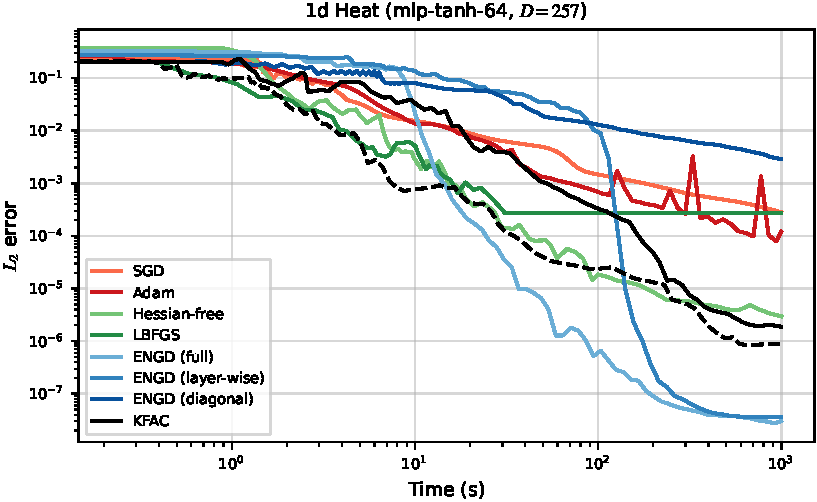
\includegraphics[trim={0 1.3cm 0 0},clip]{\pathToFigs/l2_error_over_time.pdf}
    % trim the legend and titles
    % [trim={left bottom right top},clip]
    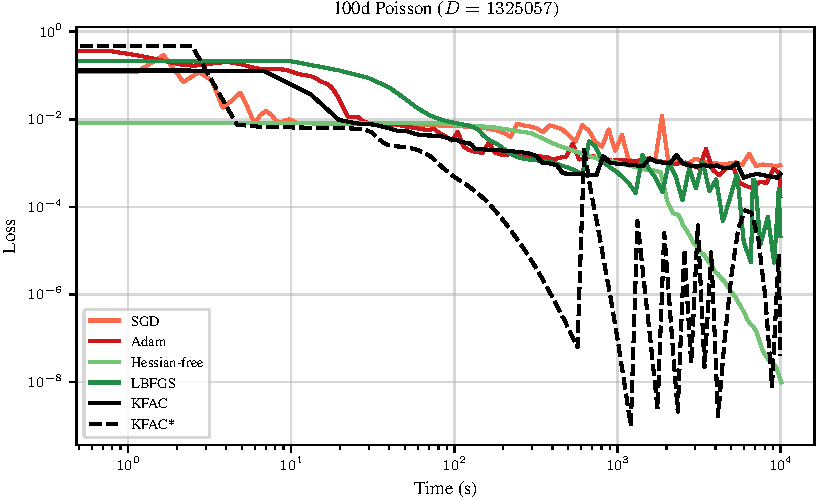
\includegraphics[trim={0 0.8cm 0 0.3cm},clip]{\pathToFigs/loss_over_time.pdf}
  \end{subfigure}
  \begin{subfigure}[t]{1.0\linewidth}
    \caption{}\label{subfig:poisson5d-step}
    % trim the legend, xlabel and xticklabels
    % [trim={left bottom right top},clip]
    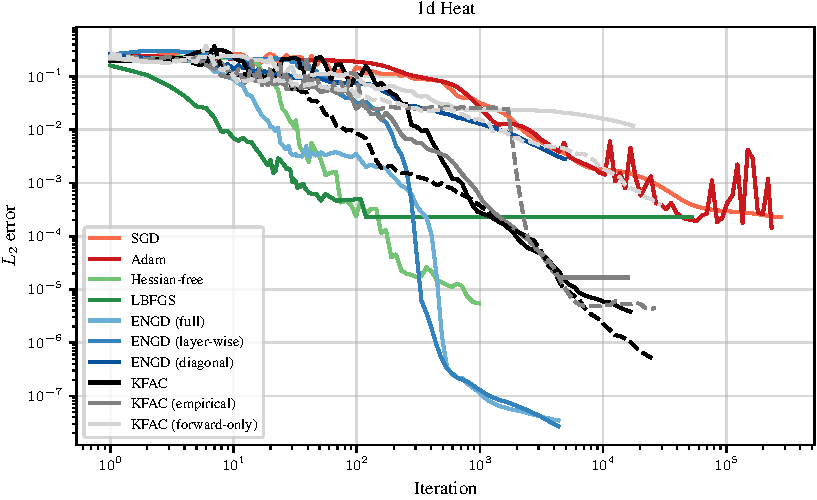
\includegraphics[trim={0 1.3cm 0 0.3cm},clip]{\pathToFigs/l2_error_over_step.pdf}
    % trim the titles
    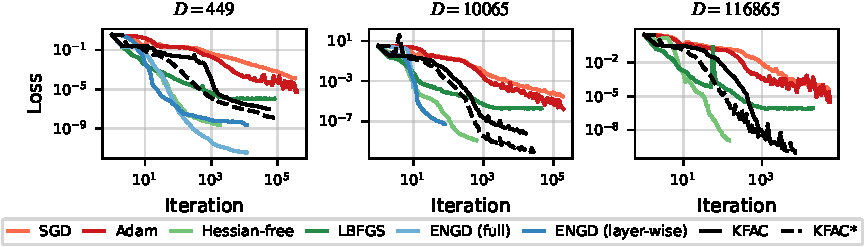
\includegraphics[trim={0 0 0 0.3cm},clip]{\pathToFigs/loss_over_step.pdf}
  \end{subfigure}
  \caption{Training loss and evaluation $L_2$ error for learning the solution to a 5d Poisson equation over (\subref{subfig:poisson5d-time}) time and (\subref{subfig:poisson5d-step}) steps.
    Columns are different neural networks.}\label{fig:poisson5d-appendix}
\end{figure}

\paragraph{Best run details}
The runs shown in \Cref{fig:poisson5d-appendix} correspond to the following hyper-parameters:
\begin{itemize}
\item $5\to 64\to 1$ MLP with $D=449$
  \begin{itemize}
    \def\pathToRuns{kfac_pinns_exp/exp10_reproduce_poisson5d/tex}
  \item \textbf{SGD:} learning rate: $\num[scientific-notation=true]{1.007555e-03}$, momentum: $\num[scientific-notation=true]{0.9}$
  \item \textbf{Adam:} learning rate: $\num[scientific-notation=true]{1.369294e-06}$, $N_{\Omega}$: $\num[scientific-notation=false]{203}$, $N_{\partial\Omega}$: $\num[scientific-notation=false]{1494}$, batch sampling frequency: $\num[scientific-notation=false]{9712}$
  \item \textbf{Hessian-free:} curvature matrix: $\text{GGN}$, initial damping: $\num[scientific-notation=true]{1.146081e-02}$, constant damping: $\text{no}$, maximum CG iterations: $\num[scientific-notation=false]{484}$, $N_{\Omega}$: $\num[scientific-notation=false]{2410}$, $N_{\partial\Omega}$: $\num[scientific-notation=false]{2448}$, batch sampling frequency: $\num[scientific-notation=false]{1311}$
  \item \textbf{LBFGS:} learning rate: $\num[scientific-notation=true]{0.2}$, history size: $\num[scientific-notation=false]{225}$
  \item \textbf{ENGD (full):} damping: $\num[scientific-notation=true]{1e-10}$, exponential moving average: $\num[scientific-notation=true]{0.3}$, initialize Gramian to identity: $\text{yes}$
  \item \textbf{ENGD (layer-wise):} damping: $\num[scientific-notation=true]{1e-06}$, exponential moving average: $\num[scientific-notation=true]{0.3}$, initialize Gramian to identity: $\text{no}$
  \item \textbf{KFAC:} damping: $\num[scientific-notation=true]{8.435180e-14}$, momentum: $\num[scientific-notation=true]{9.718645e-01}$, exponential moving average: $\num[scientific-notation=true]{9.800744e-01}$, initialize Kronecker factors to identity: $\text{yes}$, $N_{\Omega}$: $\num[scientific-notation=false]{2525}$, $N_{\partial\Omega}$: $\num[scientific-notation=false]{2663}$, batch sampling frequency: $\num[scientific-notation=false]{7916}$
  \item \textbf{KFAC*:} damping: $\num[scientific-notation=true]{2.965060e-08}$, exponential moving average: $\num[scientific-notation=true]{9.574717e-01}$, initialize Kronecker factors to identity: $\text{yes}$
  \end{itemize}

\item $5 \to 64 \to 64 \to 48 \to 48 \to 1$ MLP with $D=\num{10065}$
  \begin{itemize}
    \def\pathToRuns{kfac_pinns_exp/exp16_poisson5d_deepwide/tex}
  \item \textbf{SGD:} learning rate: $\num[scientific-notation=true]{1.007555e-03}$, momentum: $\num[scientific-notation=true]{0.9}$
  \item \textbf{Adam:} learning rate: $\num[scientific-notation=true]{1.369294e-06}$, $N_{\Omega}$: $\num[scientific-notation=false]{203}$, $N_{\partial\Omega}$: $\num[scientific-notation=false]{1494}$, batch sampling frequency: $\num[scientific-notation=false]{9712}$
  \item \textbf{Hessian-free:} curvature matrix: $\text{GGN}$, initial damping: $\num[scientific-notation=true]{1.146081e-02}$, constant damping: $\text{no}$, maximum CG iterations: $\num[scientific-notation=false]{484}$, $N_{\Omega}$: $\num[scientific-notation=false]{2410}$, $N_{\partial\Omega}$: $\num[scientific-notation=false]{2448}$, batch sampling frequency: $\num[scientific-notation=false]{1311}$
  \item \textbf{LBFGS:} learning rate: $\num[scientific-notation=true]{0.2}$, history size: $\num[scientific-notation=false]{225}$
  \item \textbf{ENGD (full):} damping: $\num[scientific-notation=true]{1e-10}$, exponential moving average: $\num[scientific-notation=true]{0.3}$, initialize Gramian to identity: $\text{yes}$
  \item \textbf{ENGD (layer-wise):} damping: $\num[scientific-notation=true]{1e-06}$, exponential moving average: $\num[scientific-notation=true]{0.3}$, initialize Gramian to identity: $\text{no}$
  \item \textbf{KFAC:} damping: $\num[scientific-notation=true]{8.435180e-14}$, momentum: $\num[scientific-notation=true]{9.718645e-01}$, exponential moving average: $\num[scientific-notation=true]{9.800744e-01}$, initialize Kronecker factors to identity: $\text{yes}$, $N_{\Omega}$: $\num[scientific-notation=false]{2525}$, $N_{\partial\Omega}$: $\num[scientific-notation=false]{2663}$, batch sampling frequency: $\num[scientific-notation=false]{7916}$
  \item \textbf{KFAC*:} damping: $\num[scientific-notation=true]{2.965060e-08}$, exponential moving average: $\num[scientific-notation=true]{9.574717e-01}$, initialize Kronecker factors to identity: $\text{yes}$
  \end{itemize}

\item $5 \to 256 \to 256\to 128 \to 128 \to 1$ MLP with $D=\num{116865}$
  \begin{itemize}
    \def\pathToRuns{kfac_pinns_exp/exp19_poisson5d_mlp_tanh_256/tex}
  \item \textbf{SGD:} learning rate: $\num[scientific-notation=true]{1.007555e-03}$, momentum: $\num[scientific-notation=true]{0.9}$
  \item \textbf{Adam:} learning rate: $\num[scientific-notation=true]{1.369294e-06}$, $N_{\Omega}$: $\num[scientific-notation=false]{203}$, $N_{\partial\Omega}$: $\num[scientific-notation=false]{1494}$, batch sampling frequency: $\num[scientific-notation=false]{9712}$
  \item \textbf{Hessian-free:} curvature matrix: $\text{GGN}$, initial damping: $\num[scientific-notation=true]{1.146081e-02}$, constant damping: $\text{no}$, maximum CG iterations: $\num[scientific-notation=false]{484}$, $N_{\Omega}$: $\num[scientific-notation=false]{2410}$, $N_{\partial\Omega}$: $\num[scientific-notation=false]{2448}$, batch sampling frequency: $\num[scientific-notation=false]{1311}$
  \item \textbf{LBFGS:} learning rate: $\num[scientific-notation=true]{0.2}$, history size: $\num[scientific-notation=false]{225}$
  \item \textbf{KFAC:} damping: $\num[scientific-notation=true]{8.435180e-14}$, momentum: $\num[scientific-notation=true]{9.718645e-01}$, exponential moving average: $\num[scientific-notation=true]{9.800744e-01}$, initialize Kronecker factors to identity: $\text{yes}$, $N_{\Omega}$: $\num[scientific-notation=false]{2525}$, $N_{\partial\Omega}$: $\num[scientific-notation=false]{2663}$, batch sampling frequency: $\num[scientific-notation=false]{7916}$
  \item \textbf{KFAC*:} damping: $\num[scientific-notation=true]{2.965060e-08}$, exponential moving average: $\num[scientific-notation=true]{9.574717e-01}$, initialize Kronecker factors to identity: $\text{yes}$
  \end{itemize}
\end{itemize}

\paragraph{Search space details} The runs shown in \Cref{fig:poisson5d-appendix} were determined to be the best via a search with approximately 50 runs on the following search spaces which were obtained by refining an initially wider search ($\mathcal{U}$ denotes a uniform, and $\mathcal{LU}$ a log-uniform distribution):
\begin{itemize}
\item $5\to 64\to 1$ MLP with $D=449$
  \begin{itemize}
    \def\pathToRuns{kfac_pinns_exp/exp10_reproduce_poisson5d/tex}
  \item \textbf{SGD:} learning rate: $\mathcal{LU}([\num[scientific-notation=true]{1e-06}; \num[scientific-notation=false]{1}])$, momentum: $\mathcal{U}([\num[scientific-notation=false]{0}; \num[scientific-notation=true]{0.99}])$, $N_{\Omega}$: $\mathcal{C}(\{\num[scientific-notation=false]{100},\num[scientific-notation=false]{101},\text{\dots},\num[scientific-notation=false]{5000}\})$, $N_{\partial\Omega}$: $\mathcal{C}(\{\num[scientific-notation=false]{50},\num[scientific-notation=false]{51},\text{\dots},\num[scientific-notation=false]{2500}\})$, batch sampling frequency: $\mathcal{C}(\{\num[scientific-notation=false]{0},\num[scientific-notation=false]{1},\text{\dots},\num[scientific-notation=false]{1000}\})$
  \item \textbf{Adam:} learning rate: $\mathcal{LU}([\num[scientific-notation=true]{0.0001}; \num[scientific-notation=true]{0.5}])$
  \item \textbf{Hessian-free:} curvature matrix: $\mathcal{U}(\{\text{GGN},\text{Hessian}\})$, initial damping: $\mathcal{LU}([\num[scientific-notation=true]{1e-15}; \num[scientific-notation=false]{1}])$, constant damping: $\mathcal{U}(\{\text{no},\text{yes}\})$, maximum CG iterations: $\mathcal{U}(\{\num[scientific-notation=false]{1},\num[scientific-notation=false]{2},\text{\dots},\num[scientific-notation=false]{500}\})$, $N_{\Omega}$: $\mathcal{U}(\{\num[scientific-notation=false]{100},\num[scientific-notation=false]{101},\text{\dots},\num[scientific-notation=false]{5000}\})$, $N_{\partial\Omega}$: $\mathcal{U}(\{\num[scientific-notation=false]{50},\num[scientific-notation=false]{51},\text{\dots},\num[scientific-notation=false]{2500}\})$, batch sampling frequency: $\mathcal{U}(\{\num[scientific-notation=false]{0},\num[scientific-notation=false]{1},\text{\dots},\num[scientific-notation=false]{5000}\})$
  \item \textbf{LBFGS:} learning rate: $\mathcal{C}(\{\num[scientific-notation=true]{0.5},\num[scientific-notation=true]{0.2},\num[scientific-notation=true]{0.1},\num[scientific-notation=true]{0.05},\num[scientific-notation=true]{0.02},\num[scientific-notation=true]{0.01}\})$, history size: $\mathcal{C}(\{\num[scientific-notation=false]{75},\num[scientific-notation=false]{100},\num[scientific-notation=false]{125},\num[scientific-notation=false]{150},\num[scientific-notation=false]{175},\num[scientific-notation=false]{200},\num[scientific-notation=false]{225},\num[scientific-notation=false]{250}\})$
  \item \textbf{ENGD (full):} damping: $\mathcal{C}(\{\num[scientific-notation=true]{1e-08},\num[scientific-notation=true]{1e-09},\num[scientific-notation=true]{1e-10},\num[scientific-notation=true]{1e-11},\num[scientific-notation=true]{1e-12},\num[scientific-notation=false]{0}\})$, exponential moving average: $\mathcal{C}(\{\num[scientific-notation=false]{0},\num[scientific-notation=true]{0.3},\num[scientific-notation=true]{0.6},\num[scientific-notation=true]{0.9}\})$, initialize Gramian to identity: $\mathcal{C}(\{\text{no},\text{yes}\})$
  \item \textbf{ENGD (layer-wise):} damping: $\mathcal{U}(\{\num[scientific-notation=true]{0.01},\num[scientific-notation=true]{0.001},\num[scientific-notation=true]{0.0001},\num[scientific-notation=true]{1e-05},\num[scientific-notation=true]{1e-06}\})$, exponential moving average: $\mathcal{U}(\{\num[scientific-notation=false]{0},\num[scientific-notation=true]{0.3},\num[scientific-notation=true]{0.6},\num[scientific-notation=true]{0.9},\num[scientific-notation=true]{0.99}\})$, initialize Gramian to identity: $\mathcal{U}(\{\text{no},\text{yes}\})$
  \item \textbf{KFAC:} damping: $\mathcal{LU}([\num[scientific-notation=true]{1e-15}; \num[scientific-notation=true]{0.01}])$, momentum: $\mathcal{U}([\num[scientific-notation=false]{0}; \num[scientific-notation=true]{0.99}])$, exponential moving average: $\mathcal{U}([\num[scientific-notation=false]{0}; \num[scientific-notation=true]{0.99}])$, initialize Kronecker factors to identity: $\mathcal{C}(\{\text{no},\text{yes}\})$
  \item \textbf{KFAC*:} damping: $\mathcal{LU}([\num[scientific-notation=true]{1e-15}; \num[scientific-notation=true]{0.01}])$, exponential moving average: $\mathcal{U}([\num[scientific-notation=false]{0}; \num[scientific-notation=true]{0.99}])$, initialize Kronecker factors to identity: $\mathcal{U}(\{\text{no},\text{yes}\})$, $N_{\Omega}$: $\mathcal{U}(\{\num[scientific-notation=false]{100},\num[scientific-notation=false]{101},\text{\dots},\num[scientific-notation=false]{5000}\})$, $N_{\partial\Omega}$: $\mathcal{U}(\{\num[scientific-notation=false]{50},\num[scientific-notation=false]{51},\text{\dots},\num[scientific-notation=false]{2500}\})$, batch sampling frequency: $\mathcal{U}(\{\num[scientific-notation=false]{0},\num[scientific-notation=false]{1},\text{\dots},\num[scientific-notation=false]{5000}\})$
  \end{itemize}

\item $5 \to 64 \to 64 \to 48 \to 48 \to 1$ MLP with $D=\num{10065}$
  \begin{itemize}
    \def\pathToRuns{kfac_pinns_exp/exp16_poisson5d_deepwide/tex}
  \item \textbf{SGD:} learning rate: $\mathcal{LU}([\num[scientific-notation=true]{1e-06}; \num[scientific-notation=false]{1}])$, momentum: $\mathcal{U}([\num[scientific-notation=false]{0}; \num[scientific-notation=true]{0.99}])$, $N_{\Omega}$: $\mathcal{C}(\{\num[scientific-notation=false]{100},\num[scientific-notation=false]{101},\text{\dots},\num[scientific-notation=false]{5000}\})$, $N_{\partial\Omega}$: $\mathcal{C}(\{\num[scientific-notation=false]{50},\num[scientific-notation=false]{51},\text{\dots},\num[scientific-notation=false]{2500}\})$, batch sampling frequency: $\mathcal{C}(\{\num[scientific-notation=false]{0},\num[scientific-notation=false]{1},\text{\dots},\num[scientific-notation=false]{1000}\})$
  \item \textbf{Adam:} learning rate: $\mathcal{LU}([\num[scientific-notation=true]{0.0001}; \num[scientific-notation=true]{0.5}])$
  \item \textbf{Hessian-free:} curvature matrix: $\mathcal{U}(\{\text{GGN},\text{Hessian}\})$, initial damping: $\mathcal{LU}([\num[scientific-notation=true]{1e-15}; \num[scientific-notation=false]{1}])$, constant damping: $\mathcal{U}(\{\text{no},\text{yes}\})$, maximum CG iterations: $\mathcal{U}(\{\num[scientific-notation=false]{1},\num[scientific-notation=false]{2},\text{\dots},\num[scientific-notation=false]{500}\})$, $N_{\Omega}$: $\mathcal{U}(\{\num[scientific-notation=false]{100},\num[scientific-notation=false]{101},\text{\dots},\num[scientific-notation=false]{5000}\})$, $N_{\partial\Omega}$: $\mathcal{U}(\{\num[scientific-notation=false]{50},\num[scientific-notation=false]{51},\text{\dots},\num[scientific-notation=false]{2500}\})$, batch sampling frequency: $\mathcal{U}(\{\num[scientific-notation=false]{0},\num[scientific-notation=false]{1},\text{\dots},\num[scientific-notation=false]{5000}\})$
  \item \textbf{LBFGS:} learning rate: $\mathcal{C}(\{\num[scientific-notation=true]{0.5},\num[scientific-notation=true]{0.2},\num[scientific-notation=true]{0.1},\num[scientific-notation=true]{0.05},\num[scientific-notation=true]{0.02},\num[scientific-notation=true]{0.01}\})$, history size: $\mathcal{C}(\{\num[scientific-notation=false]{75},\num[scientific-notation=false]{100},\num[scientific-notation=false]{125},\num[scientific-notation=false]{150},\num[scientific-notation=false]{175},\num[scientific-notation=false]{200},\num[scientific-notation=false]{225},\num[scientific-notation=false]{250}\})$
  \item \textbf{ENGD (full):} damping: $\mathcal{C}(\{\num[scientific-notation=true]{1e-08},\num[scientific-notation=true]{1e-09},\num[scientific-notation=true]{1e-10},\num[scientific-notation=true]{1e-11},\num[scientific-notation=true]{1e-12},\num[scientific-notation=false]{0}\})$, exponential moving average: $\mathcal{C}(\{\num[scientific-notation=false]{0},\num[scientific-notation=true]{0.3},\num[scientific-notation=true]{0.6},\num[scientific-notation=true]{0.9}\})$, initialize Gramian to identity: $\mathcal{C}(\{\text{no},\text{yes}\})$
  \item \textbf{ENGD (layer-wise):} damping: $\mathcal{U}(\{\num[scientific-notation=true]{0.01},\num[scientific-notation=true]{0.001},\num[scientific-notation=true]{0.0001},\num[scientific-notation=true]{1e-05},\num[scientific-notation=true]{1e-06}\})$, exponential moving average: $\mathcal{U}(\{\num[scientific-notation=false]{0},\num[scientific-notation=true]{0.3},\num[scientific-notation=true]{0.6},\num[scientific-notation=true]{0.9},\num[scientific-notation=true]{0.99}\})$, initialize Gramian to identity: $\mathcal{U}(\{\text{no},\text{yes}\})$
  \item \textbf{KFAC:} damping: $\mathcal{LU}([\num[scientific-notation=true]{1e-15}; \num[scientific-notation=true]{0.01}])$, momentum: $\mathcal{U}([\num[scientific-notation=false]{0}; \num[scientific-notation=true]{0.99}])$, exponential moving average: $\mathcal{U}([\num[scientific-notation=false]{0}; \num[scientific-notation=true]{0.99}])$, initialize Kronecker factors to identity: $\mathcal{C}(\{\text{no},\text{yes}\})$
  \item \textbf{KFAC*:} damping: $\mathcal{LU}([\num[scientific-notation=true]{1e-15}; \num[scientific-notation=true]{0.01}])$, exponential moving average: $\mathcal{U}([\num[scientific-notation=false]{0}; \num[scientific-notation=true]{0.99}])$, initialize Kronecker factors to identity: $\mathcal{U}(\{\text{no},\text{yes}\})$, $N_{\Omega}$: $\mathcal{U}(\{\num[scientific-notation=false]{100},\num[scientific-notation=false]{101},\text{\dots},\num[scientific-notation=false]{5000}\})$, $N_{\partial\Omega}$: $\mathcal{U}(\{\num[scientific-notation=false]{50},\num[scientific-notation=false]{51},\text{\dots},\num[scientific-notation=false]{2500}\})$, batch sampling frequency: $\mathcal{U}(\{\num[scientific-notation=false]{0},\num[scientific-notation=false]{1},\text{\dots},\num[scientific-notation=false]{5000}\})$
  \end{itemize}

\item $5 \to 256 \to 256\to 128 \to 128 \to 1$ MLP with $D=\num{116865}$
  \begin{itemize}
    \def\pathToRuns{kfac_pinns_exp/exp19_poisson5d_mlp_tanh_256/tex}
  \item \textbf{SGD:} learning rate: $\mathcal{LU}([\num[scientific-notation=true]{1e-06}; \num[scientific-notation=false]{1}])$, momentum: $\mathcal{U}([\num[scientific-notation=false]{0}; \num[scientific-notation=true]{0.99}])$, $N_{\Omega}$: $\mathcal{C}(\{\num[scientific-notation=false]{100},\num[scientific-notation=false]{101},\text{\dots},\num[scientific-notation=false]{5000}\})$, $N_{\partial\Omega}$: $\mathcal{C}(\{\num[scientific-notation=false]{50},\num[scientific-notation=false]{51},\text{\dots},\num[scientific-notation=false]{2500}\})$, batch sampling frequency: $\mathcal{C}(\{\num[scientific-notation=false]{0},\num[scientific-notation=false]{1},\text{\dots},\num[scientific-notation=false]{1000}\})$
  \item \textbf{Adam:} learning rate: $\mathcal{LU}([\num[scientific-notation=true]{0.0001}; \num[scientific-notation=true]{0.5}])$
  \item \textbf{Hessian-free:} curvature matrix: $\mathcal{U}(\{\text{GGN},\text{Hessian}\})$, initial damping: $\mathcal{LU}([\num[scientific-notation=true]{1e-15}; \num[scientific-notation=false]{1}])$, constant damping: $\mathcal{U}(\{\text{no},\text{yes}\})$, maximum CG iterations: $\mathcal{U}(\{\num[scientific-notation=false]{1},\num[scientific-notation=false]{2},\text{\dots},\num[scientific-notation=false]{500}\})$, $N_{\Omega}$: $\mathcal{U}(\{\num[scientific-notation=false]{100},\num[scientific-notation=false]{101},\text{\dots},\num[scientific-notation=false]{5000}\})$, $N_{\partial\Omega}$: $\mathcal{U}(\{\num[scientific-notation=false]{50},\num[scientific-notation=false]{51},\text{\dots},\num[scientific-notation=false]{2500}\})$, batch sampling frequency: $\mathcal{U}(\{\num[scientific-notation=false]{0},\num[scientific-notation=false]{1},\text{\dots},\num[scientific-notation=false]{5000}\})$
  \item \textbf{LBFGS:} learning rate: $\mathcal{C}(\{\num[scientific-notation=true]{0.5},\num[scientific-notation=true]{0.2},\num[scientific-notation=true]{0.1},\num[scientific-notation=true]{0.05},\num[scientific-notation=true]{0.02},\num[scientific-notation=true]{0.01}\})$, history size: $\mathcal{C}(\{\num[scientific-notation=false]{75},\num[scientific-notation=false]{100},\num[scientific-notation=false]{125},\num[scientific-notation=false]{150},\num[scientific-notation=false]{175},\num[scientific-notation=false]{200},\num[scientific-notation=false]{225},\num[scientific-notation=false]{250}\})$
  \item \textbf{KFAC:} damping: $\mathcal{LU}([\num[scientific-notation=true]{1e-15}; \num[scientific-notation=true]{0.01}])$, momentum: $\mathcal{U}([\num[scientific-notation=false]{0}; \num[scientific-notation=true]{0.99}])$, exponential moving average: $\mathcal{U}([\num[scientific-notation=false]{0}; \num[scientific-notation=true]{0.99}])$, initialize Kronecker factors to identity: $\mathcal{C}(\{\text{no},\text{yes}\})$
  \item \textbf{KFAC*:} damping: $\mathcal{LU}([\num[scientific-notation=true]{1e-15}; \num[scientific-notation=true]{0.01}])$, exponential moving average: $\mathcal{U}([\num[scientific-notation=false]{0}; \num[scientific-notation=true]{0.99}])$, initialize Kronecker factors to identity: $\mathcal{U}(\{\text{no},\text{yes}\})$, $N_{\Omega}$: $\mathcal{U}(\{\num[scientific-notation=false]{100},\num[scientific-notation=false]{101},\text{\dots},\num[scientific-notation=false]{5000}\})$, $N_{\partial\Omega}$: $\mathcal{U}(\{\num[scientific-notation=false]{50},\num[scientific-notation=false]{51},\text{\dots},\num[scientific-notation=false]{2500}\})$, batch sampling frequency: $\mathcal{U}(\{\num[scientific-notation=false]{0},\num[scientific-notation=false]{1},\text{\dots},\num[scientific-notation=false]{5000}\})$
  \end{itemize}
\end{itemize}

\subsection{10d Poisson Equation}\label{sec:poisson10d-appendix}

\paragraph{Setup} We consider a 10-dimensional Poisson equation $-\Delta u(\vx) = 0$ on the 10-dimensional unit square $\vx \in [0, 1]^5$ with zero right-hand side and harmonic mixed second order polynomial boundary conditions $u(\vx) = \sum_{i=1}^{\nicefrac{d}{2}} \evx_{2i-1} \evx_{2i}$ for $\vx \in \partial [0,1]^d$.
We sample training batches of size $N_{\Omega} = \num{3000}, N_{\partial\Omega} = 1000$ and evaluate the $L_2$ error on a separate set of $\num{30000}$ data points using the known solution $u_{\star}(\vx) = \sum_{i=1}^{\nicefrac{d}{2}} \evx_{2i-1} \evx_{2i}$.
All optimizers except for KFAC sample a new training batch each iteration.
KFAC only re-samples every 100 iterations because we noticed significant improvement with multiple iterations on a fixed batch.
Each run is limited to $\num{6000}\,\text{s}$.
We use a $10 \to 256 \to 256\to 128 \to 128 \to 1$ MLP with $D=\num{118145}$ MLP whose linear layers are Tanh-activated except for the final one.
\Cref{fig:poisson_10d-appendix} visualizes the results.

\begin{figure}[!h]
  \centering
  \def\pathToFigs{kfac_pinns_exp/exp21_poisson_10d}
  \begin{subfigure}[t]{1.0\linewidth}
    \caption{}\label{subfig:poisson_10d-time}
    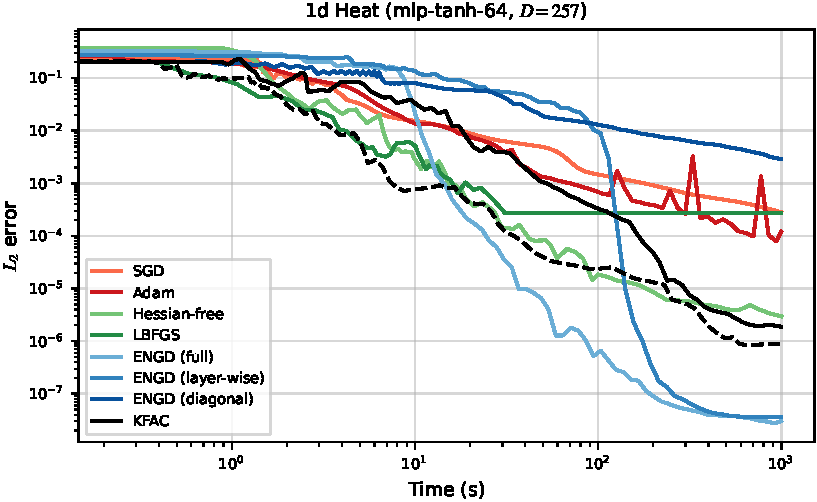
\includegraphics{\pathToFigs/l2_error_over_time.pdf}
    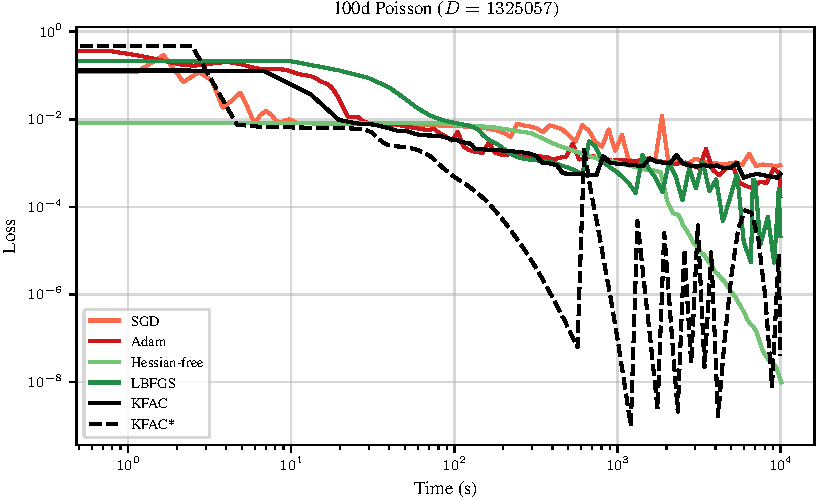
\includegraphics{\pathToFigs/loss_over_time.pdf}
  \end{subfigure}
  \begin{subfigure}[t]{1.0\linewidth}
    \caption{}\label{subfig:poisson_10d-step}
    \includegraphics{\pathToFigs/l2_error_over_step.pdf}
    \includegraphics{\pathToFigs/loss_over_step.pdf}
  \end{subfigure}
  \caption{Training loss and evaluation $L_2$ error for learning the solution to a 10d Poisson equation over (\subref{subfig:poisson_10d-time}) time and (\subref{subfig:poisson_10d-step}) steps.}\label{fig:poisson_10d-appendix}
\end{figure}

\paragraph{Best run details}
The runs shown in \Cref{fig:poisson_10d-appendix} correspond to the following hyper-parameters:
\begin{itemize}
  \def\pathToRuns{kfac_pinns_exp/exp21_poisson_10d/tex/}
\item \textbf{SGD:} learning rate: $\num[scientific-notation=true]{1.007555e-03}$, momentum: $\num[scientific-notation=true]{0.9}$
\item \textbf{Adam:} learning rate: $\num[scientific-notation=true]{1.369294e-06}$, $N_{\Omega}$: $\num[scientific-notation=false]{203}$, $N_{\partial\Omega}$: $\num[scientific-notation=false]{1494}$, batch sampling frequency: $\num[scientific-notation=false]{9712}$
\item \textbf{Hessian-free:} curvature matrix: $\text{GGN}$, initial damping: $\num[scientific-notation=true]{1.146081e-02}$, constant damping: $\text{no}$, maximum CG iterations: $\num[scientific-notation=false]{484}$, $N_{\Omega}$: $\num[scientific-notation=false]{2410}$, $N_{\partial\Omega}$: $\num[scientific-notation=false]{2448}$, batch sampling frequency: $\num[scientific-notation=false]{1311}$
\item \textbf{LBFGS:} learning rate: $\num[scientific-notation=true]{0.2}$, history size: $\num[scientific-notation=false]{225}$
\item \textbf{KFAC:} damping: $\num[scientific-notation=true]{8.435180e-14}$, momentum: $\num[scientific-notation=true]{9.718645e-01}$, exponential moving average: $\num[scientific-notation=true]{9.800744e-01}$, initialize Kronecker factors to identity: $\text{yes}$, $N_{\Omega}$: $\num[scientific-notation=false]{2525}$, $N_{\partial\Omega}$: $\num[scientific-notation=false]{2663}$, batch sampling frequency: $\num[scientific-notation=false]{7916}$
\item \textbf{KFAC*:} damping: $\num[scientific-notation=true]{2.965060e-08}$, exponential moving average: $\num[scientific-notation=true]{9.574717e-01}$, initialize Kronecker factors to identity: $\text{yes}$
\end{itemize}

\paragraph{Search space details} The runs shown in \Cref{fig:poisson_10d-appendix} were determined to be the best via a Bayesian search on the following search spaces which each optimizer given approximately the same total computational time ($\mathcal{U}$ denotes a uniform, and $\mathcal{LU}$ a log-uniform distribution):
\begin{itemize}
  \def\pathToRuns{kfac_pinns_exp/exp21_poisson_10d/tex/}
\item \textbf{SGD:} learning rate: $\mathcal{LU}([\num[scientific-notation=true]{1e-06}; \num[scientific-notation=false]{1}])$, momentum: $\mathcal{U}([\num[scientific-notation=false]{0}; \num[scientific-notation=true]{0.99}])$, $N_{\Omega}$: $\mathcal{C}(\{\num[scientific-notation=false]{100},\num[scientific-notation=false]{101},\text{\dots},\num[scientific-notation=false]{5000}\})$, $N_{\partial\Omega}$: $\mathcal{C}(\{\num[scientific-notation=false]{50},\num[scientific-notation=false]{51},\text{\dots},\num[scientific-notation=false]{2500}\})$, batch sampling frequency: $\mathcal{C}(\{\num[scientific-notation=false]{0},\num[scientific-notation=false]{1},\text{\dots},\num[scientific-notation=false]{1000}\})$
\item \textbf{Adam:} learning rate: $\mathcal{LU}([\num[scientific-notation=true]{0.0001}; \num[scientific-notation=true]{0.5}])$
\item \textbf{Hessian-free:} curvature matrix: $\mathcal{U}(\{\text{GGN},\text{Hessian}\})$, initial damping: $\mathcal{LU}([\num[scientific-notation=true]{1e-15}; \num[scientific-notation=false]{1}])$, constant damping: $\mathcal{U}(\{\text{no},\text{yes}\})$, maximum CG iterations: $\mathcal{U}(\{\num[scientific-notation=false]{1},\num[scientific-notation=false]{2},\text{\dots},\num[scientific-notation=false]{500}\})$, $N_{\Omega}$: $\mathcal{U}(\{\num[scientific-notation=false]{100},\num[scientific-notation=false]{101},\text{\dots},\num[scientific-notation=false]{5000}\})$, $N_{\partial\Omega}$: $\mathcal{U}(\{\num[scientific-notation=false]{50},\num[scientific-notation=false]{51},\text{\dots},\num[scientific-notation=false]{2500}\})$, batch sampling frequency: $\mathcal{U}(\{\num[scientific-notation=false]{0},\num[scientific-notation=false]{1},\text{\dots},\num[scientific-notation=false]{5000}\})$
\item \textbf{LBFGS:} learning rate: $\mathcal{C}(\{\num[scientific-notation=true]{0.5},\num[scientific-notation=true]{0.2},\num[scientific-notation=true]{0.1},\num[scientific-notation=true]{0.05},\num[scientific-notation=true]{0.02},\num[scientific-notation=true]{0.01}\})$, history size: $\mathcal{C}(\{\num[scientific-notation=false]{75},\num[scientific-notation=false]{100},\num[scientific-notation=false]{125},\num[scientific-notation=false]{150},\num[scientific-notation=false]{175},\num[scientific-notation=false]{200},\num[scientific-notation=false]{225},\num[scientific-notation=false]{250}\})$
\item \textbf{KFAC:} damping: $\mathcal{LU}([\num[scientific-notation=true]{1e-15}; \num[scientific-notation=true]{0.01}])$, momentum: $\mathcal{U}([\num[scientific-notation=false]{0}; \num[scientific-notation=true]{0.99}])$, exponential moving average: $\mathcal{U}([\num[scientific-notation=false]{0}; \num[scientific-notation=true]{0.99}])$, initialize Kronecker factors to identity: $\mathcal{C}(\{\text{no},\text{yes}\})$
\item \textbf{KFAC*:} damping: $\mathcal{LU}([\num[scientific-notation=true]{1e-15}; \num[scientific-notation=true]{0.01}])$, exponential moving average: $\mathcal{U}([\num[scientific-notation=false]{0}; \num[scientific-notation=true]{0.99}])$, initialize Kronecker factors to identity: $\mathcal{U}(\{\text{no},\text{yes}\})$, $N_{\Omega}$: $\mathcal{U}(\{\num[scientific-notation=false]{100},\num[scientific-notation=false]{101},\text{\dots},\num[scientific-notation=false]{5000}\})$, $N_{\partial\Omega}$: $\mathcal{U}(\{\num[scientific-notation=false]{50},\num[scientific-notation=false]{51},\text{\dots},\num[scientific-notation=false]{2500}\})$, batch sampling frequency: $\mathcal{U}(\{\num[scientific-notation=false]{0},\num[scientific-notation=false]{1},\text{\dots},\num[scientific-notation=false]{5000}\})$
\end{itemize}

\subsection{5/10/100-d Poisson Equations with Bayesian Search}\label{sec:high-dimensional-poissons-app}

\paragraph{Setup} Here, we consider three Poisson equations $- \Delta u(\vx) = f(\vx)$ with different right-hand sides and boundary conditions on the unit square $\vx \in [0, 1]^d$:
\begin{itemize}
\item $d=5$ with cosine sum right-hand side $f(\vx) = \pi^2 \sum_{i=1}^d \cos(\pi \evx_i)$, boundary conditions $u(\vx) = \sum_{i=1}^d \cos(\pi \evx_i)$ for $\vx \in \partial [0,1]^d$, and known solution $u_{\star}(\vx) = \sum_{i=1}^d \cos(\pi \evx_i)$.
  We assign each run a budget of $\num{3000}\,\text{s}$.

\item $d=10$ with zero right-hand side $f(\vx) = 0$, harmonic mixed second order polynomial boundary conditions $u(\vx) = \sum_{i=1}^{\nicefrac{d}{2}} \evx_{2i-1} \evx_{2i}$ for $\vx \in \partial [0,1]^d$, and known solution $u_{\star}(\vx) =  \sum_{i=1}^{\nicefrac{d}{2}} \evx_{2i-1} \evx_{2i}$.
  We assign each run a budget of $\num{6000}\,\text{s}$.

\item $d=100$ with constant non-zero right-hand side $f(\vx) = -2 d$, square norm boundary conditions $u(\vx) = \left\lVert \vx \right\rVert_2^2$ for $\vx \in \partial [0,1]^d$, and known solution $u_{\star}(\vx) =  \left\lVert \vx \right\rVert_2^2$.
  We assign each run a budget of $\num{10000}\,\text{s}$.
\end{itemize}
We tune the optimizer-hyperparameters described in \Cref{sec:tuning-protocol}, as well as the batch sizes $N_{\Omega}, N_{\partial \Omega}$, and their associated re-sampling frequencies using Bayesian search.
We use five layer MLP architectures with varying widths whose layers are Tanh-activated except for the final layer.
These architectures are too large to be optimized by ENGD.
\Cref{fig:poisson-bayes-appendix} visualizes the results.

\begin{figure}[!h]
  \centering
  \def\pathToFigs{kfac_pinns_exp/exp33_poisson_bayes_groupplot}
  \begin{subfigure}[t]{1.0\linewidth}
    \caption{}\label{subfig:poisson-bayes-time}
    % trim legend, xlabel and xticklabels
    % [trim={left bottom right top},clip]
    \includegraphics[trim={0 1.3cm 0 0},clip]{\pathToFigs/l2_error_over_time.pdf}
    % trim the legend and titles
    % [trim={left bottom right top},clip]
    \includegraphics[trim={0 0.5cm 0 0.3cm},clip]{\pathToFigs/loss_over_time.pdf}
  \end{subfigure}
  \begin{subfigure}[t]{1.0\linewidth}
    \caption{}\label{subfig:poisson-bayes-step}
    % trim the legend, xlabel and xticklabels
    % [trim={left bottom right top},clip]
    \includegraphics[trim={0 1.3cm 0 0.3cm},clip]{\pathToFigs/l2_error_over_step.pdf}
    % trim the titles
    \includegraphics[trim={0 0 0 0.3cm},clip]{\pathToFigs/loss_over_step.pdf}
  \end{subfigure}
  \caption{Training loss and evaluation $L_2$ error for learning the solution to high-dimensional Poisson equations over (\subref{subfig:poisson-bayes-time}) time and (\subref{subfig:poisson-bayes-step}) steps using Bayesian search.}\label{fig:poisson-bayes-appendix}
\end{figure}

\paragraph{Best run details} The runs shown in \Cref{fig:poisson-bayes-appendix} correspond to the following hyper-parameters:

\begin{itemize}

\item 5d Poisson equation, $5 \to 256 \to 256 \to 128 \to 128 \to 1$ MLP with $D=\num{116865}$
  \begin{itemize}
    \def\pathToRuns{kfac_pinns_exp/exp26_poisson5d_mlp_tanh_256_bayes/tex}
  \item \textbf{SGD:} learning rate: $\num[scientific-notation=true]{1.007555e-03}$, momentum: $\num[scientific-notation=true]{0.9}$
  \item \textbf{Adam:} learning rate: $\num[scientific-notation=true]{1.369294e-06}$, $N_{\Omega}$: $\num[scientific-notation=false]{203}$, $N_{\partial\Omega}$: $\num[scientific-notation=false]{1494}$, batch sampling frequency: $\num[scientific-notation=false]{9712}$
  \item \textbf{Hessian-free:} curvature matrix: $\text{GGN}$, initial damping: $\num[scientific-notation=true]{1.146081e-02}$, constant damping: $\text{no}$, maximum CG iterations: $\num[scientific-notation=false]{484}$, $N_{\Omega}$: $\num[scientific-notation=false]{2410}$, $N_{\partial\Omega}$: $\num[scientific-notation=false]{2448}$, batch sampling frequency: $\num[scientific-notation=false]{1311}$
  \item \textbf{LBFGS:} learning rate: $\num[scientific-notation=true]{0.2}$, history size: $\num[scientific-notation=false]{225}$
  \item \textbf{KFAC:} damping: $\num[scientific-notation=true]{8.435180e-14}$, momentum: $\num[scientific-notation=true]{9.718645e-01}$, exponential moving average: $\num[scientific-notation=true]{9.800744e-01}$, initialize Kronecker factors to identity: $\text{yes}$, $N_{\Omega}$: $\num[scientific-notation=false]{2525}$, $N_{\partial\Omega}$: $\num[scientific-notation=false]{2663}$, batch sampling frequency: $\num[scientific-notation=false]{7916}$
  \item \textbf{KFAC*:} damping: $\num[scientific-notation=true]{2.965060e-08}$, exponential moving average: $\num[scientific-notation=true]{9.574717e-01}$, initialize Kronecker factors to identity: $\text{yes}$
  \end{itemize}

\item 10d Poisson equation, $10 \to 256 \to 256 \to 128 \to 128 \to 1$ MLP with $D=\num{118145}$
  \begin{itemize}
    \def\pathToRuns{kfac_pinns_exp/exp32_poisson10d_mlp_tanh_256_bayes/tex}
  \item \textbf{SGD:} learning rate: $\num[scientific-notation=true]{1.007555e-03}$, momentum: $\num[scientific-notation=true]{0.9}$
  \item \textbf{Adam:} learning rate: $\num[scientific-notation=true]{1.369294e-06}$, $N_{\Omega}$: $\num[scientific-notation=false]{203}$, $N_{\partial\Omega}$: $\num[scientific-notation=false]{1494}$, batch sampling frequency: $\num[scientific-notation=false]{9712}$
  \item \textbf{Hessian-free:} curvature matrix: $\text{GGN}$, initial damping: $\num[scientific-notation=true]{1.146081e-02}$, constant damping: $\text{no}$, maximum CG iterations: $\num[scientific-notation=false]{484}$, $N_{\Omega}$: $\num[scientific-notation=false]{2410}$, $N_{\partial\Omega}$: $\num[scientific-notation=false]{2448}$, batch sampling frequency: $\num[scientific-notation=false]{1311}$
  \item \textbf{LBFGS:} learning rate: $\num[scientific-notation=true]{0.2}$, history size: $\num[scientific-notation=false]{225}$
  \item \textbf{KFAC:} damping: $\num[scientific-notation=true]{8.435180e-14}$, momentum: $\num[scientific-notation=true]{9.718645e-01}$, exponential moving average: $\num[scientific-notation=true]{9.800744e-01}$, initialize Kronecker factors to identity: $\text{yes}$, $N_{\Omega}$: $\num[scientific-notation=false]{2525}$, $N_{\partial\Omega}$: $\num[scientific-notation=false]{2663}$, batch sampling frequency: $\num[scientific-notation=false]{7916}$
  \item \textbf{KFAC*:} damping: $\num[scientific-notation=true]{2.965060e-08}$, exponential moving average: $\num[scientific-notation=true]{9.574717e-01}$, initialize Kronecker factors to identity: $\text{yes}$
  \end{itemize}

\item 100d Poisson equation, $100 \to 768 \to 768 \to 512 \to 512 \to 1$ MLP with $D=\num{1325057}$
  \begin{itemize}
    \def\pathToRuns{kfac_pinns_exp/exp14_poisson_100d_weinan/tex}
  \item \textbf{SGD:} learning rate: $\num[scientific-notation=true]{1.007555e-03}$, momentum: $\num[scientific-notation=true]{0.9}$
  \item \textbf{Adam:} learning rate: $\num[scientific-notation=true]{1.369294e-06}$, $N_{\Omega}$: $\num[scientific-notation=false]{203}$, $N_{\partial\Omega}$: $\num[scientific-notation=false]{1494}$, batch sampling frequency: $\num[scientific-notation=false]{9712}$
  \item \textbf{Hessian-free:} curvature matrix: $\text{GGN}$, initial damping: $\num[scientific-notation=true]{1.146081e-02}$, constant damping: $\text{no}$, maximum CG iterations: $\num[scientific-notation=false]{484}$, $N_{\Omega}$: $\num[scientific-notation=false]{2410}$, $N_{\partial\Omega}$: $\num[scientific-notation=false]{2448}$, batch sampling frequency: $\num[scientific-notation=false]{1311}$
  \item \textbf{LBFGS:} learning rate: $\num[scientific-notation=true]{0.2}$, history size: $\num[scientific-notation=false]{225}$
  \item \textbf{KFAC:} damping: $\num[scientific-notation=true]{8.435180e-14}$, momentum: $\num[scientific-notation=true]{9.718645e-01}$, exponential moving average: $\num[scientific-notation=true]{9.800744e-01}$, initialize Kronecker factors to identity: $\text{yes}$, $N_{\Omega}$: $\num[scientific-notation=false]{2525}$, $N_{\partial\Omega}$: $\num[scientific-notation=false]{2663}$, batch sampling frequency: $\num[scientific-notation=false]{7916}$
  \item \textbf{KFAC*:} damping: $\num[scientific-notation=true]{2.965060e-08}$, exponential moving average: $\num[scientific-notation=true]{9.574717e-01}$, initialize Kronecker factors to identity: $\text{yes}$
  \end{itemize}
\end{itemize}

\paragraph{Search space details} The runs shown in \Cref{fig:poisson-bayes-appendix} were determined to be the best via a Bayesian search on the following search spaces which each optimizer given approximately the same total computational time ($\mathcal{U}$ denotes a uniform, and $\mathcal{LU}$ a log-uniform distribution):
\begin{itemize}

\item 5d Poisson equation, $5 \to 256 \to 256 \to 128 \to 128 \to 1$ MLP with $D=\num{116865}$
  \begin{itemize}
    \def\pathToRuns{kfac_pinns_exp/exp26_poisson5d_mlp_tanh_256_bayes/tex}
  \item \textbf{SGD:} learning rate: $\mathcal{LU}([\num[scientific-notation=true]{1e-06}; \num[scientific-notation=false]{1}])$, momentum: $\mathcal{U}([\num[scientific-notation=false]{0}; \num[scientific-notation=true]{0.99}])$, $N_{\Omega}$: $\mathcal{C}(\{\num[scientific-notation=false]{100},\num[scientific-notation=false]{101},\text{\dots},\num[scientific-notation=false]{5000}\})$, $N_{\partial\Omega}$: $\mathcal{C}(\{\num[scientific-notation=false]{50},\num[scientific-notation=false]{51},\text{\dots},\num[scientific-notation=false]{2500}\})$, batch sampling frequency: $\mathcal{C}(\{\num[scientific-notation=false]{0},\num[scientific-notation=false]{1},\text{\dots},\num[scientific-notation=false]{1000}\})$
  \item \textbf{Adam:} learning rate: $\mathcal{LU}([\num[scientific-notation=true]{0.0001}; \num[scientific-notation=true]{0.5}])$
  \item \textbf{Hessian-free:} curvature matrix: $\mathcal{U}(\{\text{GGN},\text{Hessian}\})$, initial damping: $\mathcal{LU}([\num[scientific-notation=true]{1e-15}; \num[scientific-notation=false]{1}])$, constant damping: $\mathcal{U}(\{\text{no},\text{yes}\})$, maximum CG iterations: $\mathcal{U}(\{\num[scientific-notation=false]{1},\num[scientific-notation=false]{2},\text{\dots},\num[scientific-notation=false]{500}\})$, $N_{\Omega}$: $\mathcal{U}(\{\num[scientific-notation=false]{100},\num[scientific-notation=false]{101},\text{\dots},\num[scientific-notation=false]{5000}\})$, $N_{\partial\Omega}$: $\mathcal{U}(\{\num[scientific-notation=false]{50},\num[scientific-notation=false]{51},\text{\dots},\num[scientific-notation=false]{2500}\})$, batch sampling frequency: $\mathcal{U}(\{\num[scientific-notation=false]{0},\num[scientific-notation=false]{1},\text{\dots},\num[scientific-notation=false]{5000}\})$
  \item \textbf{LBFGS:} learning rate: $\mathcal{C}(\{\num[scientific-notation=true]{0.5},\num[scientific-notation=true]{0.2},\num[scientific-notation=true]{0.1},\num[scientific-notation=true]{0.05},\num[scientific-notation=true]{0.02},\num[scientific-notation=true]{0.01}\})$, history size: $\mathcal{C}(\{\num[scientific-notation=false]{75},\num[scientific-notation=false]{100},\num[scientific-notation=false]{125},\num[scientific-notation=false]{150},\num[scientific-notation=false]{175},\num[scientific-notation=false]{200},\num[scientific-notation=false]{225},\num[scientific-notation=false]{250}\})$
  \item \textbf{KFAC:} damping: $\mathcal{LU}([\num[scientific-notation=true]{1e-15}; \num[scientific-notation=true]{0.01}])$, momentum: $\mathcal{U}([\num[scientific-notation=false]{0}; \num[scientific-notation=true]{0.99}])$, exponential moving average: $\mathcal{U}([\num[scientific-notation=false]{0}; \num[scientific-notation=true]{0.99}])$, initialize Kronecker factors to identity: $\mathcal{C}(\{\text{no},\text{yes}\})$
  \item \textbf{KFAC*:} damping: $\mathcal{LU}([\num[scientific-notation=true]{1e-15}; \num[scientific-notation=true]{0.01}])$, exponential moving average: $\mathcal{U}([\num[scientific-notation=false]{0}; \num[scientific-notation=true]{0.99}])$, initialize Kronecker factors to identity: $\mathcal{U}(\{\text{no},\text{yes}\})$, $N_{\Omega}$: $\mathcal{U}(\{\num[scientific-notation=false]{100},\num[scientific-notation=false]{101},\text{\dots},\num[scientific-notation=false]{5000}\})$, $N_{\partial\Omega}$: $\mathcal{U}(\{\num[scientific-notation=false]{50},\num[scientific-notation=false]{51},\text{\dots},\num[scientific-notation=false]{2500}\})$, batch sampling frequency: $\mathcal{U}(\{\num[scientific-notation=false]{0},\num[scientific-notation=false]{1},\text{\dots},\num[scientific-notation=false]{5000}\})$
  \end{itemize}

\item 10d Poisson equation, $10 \to 256 \to 256 \to 128 \to 128 \to 1$ MLP with $D=\num{118145}$
  \begin{itemize}
    \def\pathToRuns{kfac_pinns_exp/exp32_poisson10d_mlp_tanh_256_bayes/tex}
  \item \textbf{SGD:} learning rate: $\mathcal{LU}([\num[scientific-notation=true]{1e-06}; \num[scientific-notation=false]{1}])$, momentum: $\mathcal{U}([\num[scientific-notation=false]{0}; \num[scientific-notation=true]{0.99}])$, $N_{\Omega}$: $\mathcal{C}(\{\num[scientific-notation=false]{100},\num[scientific-notation=false]{101},\text{\dots},\num[scientific-notation=false]{5000}\})$, $N_{\partial\Omega}$: $\mathcal{C}(\{\num[scientific-notation=false]{50},\num[scientific-notation=false]{51},\text{\dots},\num[scientific-notation=false]{2500}\})$, batch sampling frequency: $\mathcal{C}(\{\num[scientific-notation=false]{0},\num[scientific-notation=false]{1},\text{\dots},\num[scientific-notation=false]{1000}\})$
  \item \textbf{Adam:} learning rate: $\mathcal{LU}([\num[scientific-notation=true]{0.0001}; \num[scientific-notation=true]{0.5}])$
  \item \textbf{Hessian-free:} curvature matrix: $\mathcal{U}(\{\text{GGN},\text{Hessian}\})$, initial damping: $\mathcal{LU}([\num[scientific-notation=true]{1e-15}; \num[scientific-notation=false]{1}])$, constant damping: $\mathcal{U}(\{\text{no},\text{yes}\})$, maximum CG iterations: $\mathcal{U}(\{\num[scientific-notation=false]{1},\num[scientific-notation=false]{2},\text{\dots},\num[scientific-notation=false]{500}\})$, $N_{\Omega}$: $\mathcal{U}(\{\num[scientific-notation=false]{100},\num[scientific-notation=false]{101},\text{\dots},\num[scientific-notation=false]{5000}\})$, $N_{\partial\Omega}$: $\mathcal{U}(\{\num[scientific-notation=false]{50},\num[scientific-notation=false]{51},\text{\dots},\num[scientific-notation=false]{2500}\})$, batch sampling frequency: $\mathcal{U}(\{\num[scientific-notation=false]{0},\num[scientific-notation=false]{1},\text{\dots},\num[scientific-notation=false]{5000}\})$
  \item \textbf{LBFGS:} learning rate: $\mathcal{C}(\{\num[scientific-notation=true]{0.5},\num[scientific-notation=true]{0.2},\num[scientific-notation=true]{0.1},\num[scientific-notation=true]{0.05},\num[scientific-notation=true]{0.02},\num[scientific-notation=true]{0.01}\})$, history size: $\mathcal{C}(\{\num[scientific-notation=false]{75},\num[scientific-notation=false]{100},\num[scientific-notation=false]{125},\num[scientific-notation=false]{150},\num[scientific-notation=false]{175},\num[scientific-notation=false]{200},\num[scientific-notation=false]{225},\num[scientific-notation=false]{250}\})$
  \item \textbf{KFAC:} damping: $\mathcal{LU}([\num[scientific-notation=true]{1e-15}; \num[scientific-notation=true]{0.01}])$, momentum: $\mathcal{U}([\num[scientific-notation=false]{0}; \num[scientific-notation=true]{0.99}])$, exponential moving average: $\mathcal{U}([\num[scientific-notation=false]{0}; \num[scientific-notation=true]{0.99}])$, initialize Kronecker factors to identity: $\mathcal{C}(\{\text{no},\text{yes}\})$
  \item \textbf{KFAC*:} damping: $\mathcal{LU}([\num[scientific-notation=true]{1e-15}; \num[scientific-notation=true]{0.01}])$, exponential moving average: $\mathcal{U}([\num[scientific-notation=false]{0}; \num[scientific-notation=true]{0.99}])$, initialize Kronecker factors to identity: $\mathcal{U}(\{\text{no},\text{yes}\})$, $N_{\Omega}$: $\mathcal{U}(\{\num[scientific-notation=false]{100},\num[scientific-notation=false]{101},\text{\dots},\num[scientific-notation=false]{5000}\})$, $N_{\partial\Omega}$: $\mathcal{U}(\{\num[scientific-notation=false]{50},\num[scientific-notation=false]{51},\text{\dots},\num[scientific-notation=false]{2500}\})$, batch sampling frequency: $\mathcal{U}(\{\num[scientific-notation=false]{0},\num[scientific-notation=false]{1},\text{\dots},\num[scientific-notation=false]{5000}\})$
  \end{itemize}

\item 100d Poisson equation, $100 \to 768 \to 768 \to 512 \to 512 \to 1$ MLP with $D=\num{1325057}$
  \begin{itemize}
    \def\pathToRuns{kfac_pinns_exp/exp14_poisson_100d_weinan/tex}
  \item \textbf{SGD:} learning rate: $\mathcal{LU}([\num[scientific-notation=true]{1e-06}; \num[scientific-notation=false]{1}])$, momentum: $\mathcal{U}([\num[scientific-notation=false]{0}; \num[scientific-notation=true]{0.99}])$, $N_{\Omega}$: $\mathcal{C}(\{\num[scientific-notation=false]{100},\num[scientific-notation=false]{101},\text{\dots},\num[scientific-notation=false]{5000}\})$, $N_{\partial\Omega}$: $\mathcal{C}(\{\num[scientific-notation=false]{50},\num[scientific-notation=false]{51},\text{\dots},\num[scientific-notation=false]{2500}\})$, batch sampling frequency: $\mathcal{C}(\{\num[scientific-notation=false]{0},\num[scientific-notation=false]{1},\text{\dots},\num[scientific-notation=false]{1000}\})$
  \item \textbf{Adam:} learning rate: $\mathcal{LU}([\num[scientific-notation=true]{0.0001}; \num[scientific-notation=true]{0.5}])$
  \item \textbf{Hessian-free:} curvature matrix: $\mathcal{U}(\{\text{GGN},\text{Hessian}\})$, initial damping: $\mathcal{LU}([\num[scientific-notation=true]{1e-15}; \num[scientific-notation=false]{1}])$, constant damping: $\mathcal{U}(\{\text{no},\text{yes}\})$, maximum CG iterations: $\mathcal{U}(\{\num[scientific-notation=false]{1},\num[scientific-notation=false]{2},\text{\dots},\num[scientific-notation=false]{500}\})$, $N_{\Omega}$: $\mathcal{U}(\{\num[scientific-notation=false]{100},\num[scientific-notation=false]{101},\text{\dots},\num[scientific-notation=false]{5000}\})$, $N_{\partial\Omega}$: $\mathcal{U}(\{\num[scientific-notation=false]{50},\num[scientific-notation=false]{51},\text{\dots},\num[scientific-notation=false]{2500}\})$, batch sampling frequency: $\mathcal{U}(\{\num[scientific-notation=false]{0},\num[scientific-notation=false]{1},\text{\dots},\num[scientific-notation=false]{5000}\})$
  \item \textbf{LBFGS:} learning rate: $\mathcal{C}(\{\num[scientific-notation=true]{0.5},\num[scientific-notation=true]{0.2},\num[scientific-notation=true]{0.1},\num[scientific-notation=true]{0.05},\num[scientific-notation=true]{0.02},\num[scientific-notation=true]{0.01}\})$, history size: $\mathcal{C}(\{\num[scientific-notation=false]{75},\num[scientific-notation=false]{100},\num[scientific-notation=false]{125},\num[scientific-notation=false]{150},\num[scientific-notation=false]{175},\num[scientific-notation=false]{200},\num[scientific-notation=false]{225},\num[scientific-notation=false]{250}\})$
  \item \textbf{KFAC:} damping: $\mathcal{LU}([\num[scientific-notation=true]{1e-15}; \num[scientific-notation=true]{0.01}])$, momentum: $\mathcal{U}([\num[scientific-notation=false]{0}; \num[scientific-notation=true]{0.99}])$, exponential moving average: $\mathcal{U}([\num[scientific-notation=false]{0}; \num[scientific-notation=true]{0.99}])$, initialize Kronecker factors to identity: $\mathcal{C}(\{\text{no},\text{yes}\})$
  \item \textbf{KFAC*:} damping: $\mathcal{LU}([\num[scientific-notation=true]{1e-15}; \num[scientific-notation=true]{0.01}])$, exponential moving average: $\mathcal{U}([\num[scientific-notation=false]{0}; \num[scientific-notation=true]{0.99}])$, initialize Kronecker factors to identity: $\mathcal{U}(\{\text{no},\text{yes}\})$, $N_{\Omega}$: $\mathcal{U}(\{\num[scientific-notation=false]{100},\num[scientific-notation=false]{101},\text{\dots},\num[scientific-notation=false]{5000}\})$, $N_{\partial\Omega}$: $\mathcal{U}(\{\num[scientific-notation=false]{50},\num[scientific-notation=false]{51},\text{\dots},\num[scientific-notation=false]{2500}\})$, batch sampling frequency: $\mathcal{U}(\{\num[scientific-notation=false]{0},\num[scientific-notation=false]{1},\text{\dots},\num[scientific-notation=false]{5000}\})$
  \end{itemize}
\end{itemize}

\subsection{PINN Loss for the Heat Equation}\label{sec:pinn-loss-heat-equation}
Consider the $D$-dimensional\todo{Low priority: lower case $d$ or upper case $D$? The number of trainable weights is already $D$.} homogeneous heat equation
\begin{align*}
  \partial_{t} u(t, \vx)
  -
  \kappa \Delta_{\vx} u(t, \vx)
  =
  0
\end{align*}
where $\vx \in \Omega \subseteq \sR^D$, $t \in \mathrm{T} \subseteq \sR$ is a time interval, and $\kappa >0$ denotes the heat conductivity. In this case, our neural network processes a $D+1$-dimensional vector $\tilde{\vx} =
\begin{pmatrix} t \\ \vx \end{pmatrix}$ and we can re-write the heat equation as
\begin{align*}
  \partial_{[\tilde{\vx}]_1} u(\tilde{\vx})
  -
  \kappa \sum_{d=2}^{D+1} \Delta_{[\tilde{\vx}]_d} u(\tilde{\vx})
  =
  0\,.
\end{align*}
In the following, we consider the unit time interval $\mathrm{T} = [0;1]$, the unit square $\Omega = [0;1]^D$ and set $\kappa = \nicefrac{1}{4}$. There are two types of constraints we need to enforce on the heat equation in order to obtain unique solutions: initial conditions and boundary conditions. As our framework for the KFAC approximation assumes only two terms in the loss function, we combine the contributions from the boundary and initial values into one term. To make this more precise consider the following example solution of the heat equation, which will be used later on as well.
As initial conditions, we use $u_0(x) = u(0, \vx) = \prod_{d=1}^D \sin(\pi [\vx_d])$ for $\vx \in \Omega$.
For boundary conditions, we use $g(t, \vx) = 0$ for $t, \vx \in \mathrm{T} \times \partial\Omega$.
The manufactured solution thus is
\begin{align*}
  u^{\star}(t, \vx)
  =
  \exp \left(-\frac{\pi^2 D t}{4} \right)
  \prod_{d=1}^D \sin(\pi [\vx_d])\,.
\end{align*}
The PINN loss for this problem consists of three terms
\begin{align*}
  \gL(\vtheta)
  &=
    \frac{1}{N_{\Omega}}
    \sum_{n=1}^{N_{\Omega}}
    \left\lVert
    \partial_t u_{\vtheta}(\tilde{\vx}_n^{\Omega})
    -
    \frac{1}{4} \Delta_{\vx} u_{\vtheta}(\tilde{\vx}_n^{\Omega})
    \right\rVert^2_2
  \\
  &+
    \frac{1}{N_{\partial\Omega}}
    \sum_{n=1}^{N_{\partial\Omega}}
    \left\lVert
    u_{\vtheta}(\tilde{\vx}_n^{\partial\Omega})
    -
    g(\tilde{\vx}_n^{\partial\Omega})
    \right\rVert^2_2
  \\
  &+
    \frac{1}{N_0}
    \sum_{n=1}^{N_0}
    \left\lVert
    u_{\vtheta}(0, \vx_n^0)
    -
    u_0( \vx_n^0)
    \right\rVert^2_2
\end{align*}
with $\tilde{\vx}_n^{\Omega} \sim \mathrm{T} \times \Omega$, and $\tilde{\vx}_n^{\partial\Omega} \sim \mathrm{T} \times \partial\Omega$, and $\vx_n^0 \sim \{0\} \times \Omega$.
To fit this loss into our framework which assumes two loss terms, each of whose curvature is approximated with a Kronecker factor, we combine the initial value and boundary value conditions into a single term.
Assuming $N_{\partial \Omega} = N_0 = \nicefrac{N_{\text{cond}}}{2}$ without loss of generality, we write
\begin{align*}
  \gL(\vtheta)
  &=
    \underbrace{
    \frac{1}{N_{\Omega}}
    \sum_{n=1}^{N_{\Omega}}
    \left\lVert
    \partial_t u_{\vtheta}(\tilde{\vx}_n^{\Omega})
    -
    \frac{1}{4} \Delta_{\vx} u_{\vtheta}(\tilde{\vx}_n^{\Omega})
    - y_n^{\Omega}
    \right\rVert^2_2
    }_{\gL_{\Omega}(\vtheta)}
  +
    \underbrace{
    \frac{1}{N_{\text{cond}}}
    \sum_{n=1}^{N_{\text{cond}}}
    \left\lVert
    u_{\vtheta}(\tilde{\vx}_n^{\text{cond}})
    -
    y_n^{\text{cond}}
    \right\rVert^2_2
    }_{\gL_{\text{cond}}(\vtheta)}
\end{align*}
with domain inputs $\tilde{\vx}_n^{\Omega} \sim \mathrm{T} \times \Omega$ and targets $y_n^{\Omega} = 0$, boundary and initial condition targets $y_n^{\text{cond}} = u(\tilde{\vx}_n^{\text{cond}})$ with initial inputs $\tilde{\vx}_n^{\text{cond}} \sim \{0\} \times \Omega$ for $n = 1, \dots, \nicefrac{N_{\text{cond}}}{2}$ and boundary inputs $\tilde{\vx}_n^{\partial\Omega} \sim \mathrm{T} \times \partial\Omega$ for $n = \nicefrac{N_{\text{cond}}}{2}+1, \dots, N_{\text{cond}}$.
The boundary and initial condition loss are of exactly same structure as the loss we discussed for the Poisson equation.

%%% Local Variables:
%%% mode: latex
%%% TeX-master: "../main"
%%% End:


\subsection{1+1d Heat Equation}\label{sec:1d-heat-equation}

\paragraph{Setup} We consider a 1+1-dimensional heat equation $\partial_tu(t,x) - \kappa \Delta_{x} u(t, x) = 0$ with $\kappa = \nicefrac{1}{4}$ on the unit square and unit time interval, $x, t \in [0,1] \times [0,1]$.
The equation has zero spatial boundary conditions and the initial values are given by $u(0, x) = \sin(\pi x)$ for $\vx \in [0,1]$.
We sample a single training batch of size $N_{\Omega} = \num{900}, N_{\partial\Omega} = 120$ ($\nicefrac{N_{\partial\Omega}}{2}$ points for the initial value and spatial boundary conditions each) and evaluate the $L_2$ error on a separate set of $\num{9000}$ data points using the known solution $u_{\star}(t, x) = \exp(-\nicefrac{\pi^2t}{4}) \sin(\pi x)$.
Each run is limited to $\num{1000}\,\text{s}$. We compare three MLP architectures of increasing size, each of whose linear layers are Tanh-activated except for the final one: a shallow $2\to 64\to 1$ MLP with $D=257$ trainable parameters, a five layer $2 \to 64 \to 64 \to 48 \to 48 \to 1$ MLP with $D=\num{9873}$ trainable parameters, and a five layer $2 \to 256 \to 256\to 128 \to 128 \to 1$ MLP with $D=\num{116097}$ trainable parameters.
For the biggest architecture, full and layer-wise ENGD lead to out-of-memory errors and are thus not part of the experiments.
Figure \Cref{fig:heat1d-appendix} summarizes the results, and \Cref{fig:1d-heat-visualization} illustrates the learned solutions over training for all optimizers on the shallow MLP

\begin{figure}[!h]
  \centering
  \def\pathToFigs{kfac_pinns_exp/exp24_heat1d_groupplot}
  \begin{subfigure}[t]{1.0\linewidth}
    \caption{}\label{subfig:heat1d-time}
    % trim legend, xlabel and xticklabels
    % [trim={left bottom right top},clip]
    \includegraphics[trim={0 1.3cm 0 0},clip]{\pathToFigs/l2_error_over_time.pdf}
    % trim the legend and titles
    % [trim={left bottom right top},clip]
    \includegraphics[trim={0 0.8cm 0 0.3cm},clip]{\pathToFigs/loss_over_time.pdf}
  \end{subfigure}
  \begin{subfigure}[t]{1.0\linewidth}
    \caption{}\label{subfig:heat1d-step}
    % trim the legend, xlabel and xticklabels
    % [trim={left bottom right top},clip]
    \includegraphics[trim={0 1.3cm 0 0.3cm},clip]{\pathToFigs/l2_error_over_step.pdf}
    % trim the titles
    \includegraphics[trim={0 0 0 0.3cm},clip]{\pathToFigs/loss_over_step.pdf}
  \end{subfigure}
  \caption{training loss and evaluation $L_2$ error for learning the solution to a 1+1-dimensional heat equation over (\subref{subfig:heat1d-time}) time and (\subref{subfig:heat1d-step}). each column corresponds to a different neural network.}\label{fig:heat1d-appendix}
\end{figure}

\begin{table}[!h]
  \begin{small}
    \centering
    \def\pathToRuns{kfac_pinns_exp/exp42_visualize_solutions/visualize_solution}
    \renewcommand\tabularxcolumn[1]{>{\Centering}m{#1}}
    \begin{tabularx}{\textwidth}{XXXXXX}
      \textbf{Optimizer} & \textbf{First step} & \textbf{0.1\% trained} & \textbf{1\% trained} & \textbf{10\% trained} & \textbf{True solution}
      \\
      SGD
      &\includegraphics[trim={0.9cm 0.8cm 6.5cm 1.0cm},clip,scale=0.31]{\pathToRuns/SGD/heat_1d_sin_product_mlp-tanh-64_SGD_step0000000.pdf}
      &\includegraphics[trim={0.9cm 0.8cm 6.5cm 1.0cm},clip,scale=0.31]{\pathToRuns/SGD/heat_1d_sin_product_mlp-tanh-64_SGD_step0000277.pdf}
      &\includegraphics[trim={0.9cm 0.8cm 6.5cm 1.0cm},clip,scale=0.31]{\pathToRuns/SGD/heat_1d_sin_product_mlp-tanh-64_SGD_step0003000.pdf}
      &\includegraphics[trim={0.9cm 0.8cm 6.5cm 1.0cm},clip,scale=0.31]{\pathToRuns/SGD/heat_1d_sin_product_mlp-tanh-64_SGD_step0029540.pdf}
      &\includegraphics[trim={7.25cm 0.8cm 0 1.0cm},clip,scale=0.31]{\pathToRuns/SGD/heat_1d_sin_product_mlp-tanh-64_SGD_step0000000.pdf}
      \\
      Adam
      % [trim={left bottom right top},clip]
      &\includegraphics[trim={0.9cm 0.8cm 6.5cm 1.0cm},clip,scale=0.31]{\pathToRuns/Adam/heat_1d_sin_product_mlp-tanh-64_Adam_step0000000.pdf}
      &\includegraphics[trim={0.9cm 0.8cm 6.5cm 1.0cm},clip,scale=0.31]{\pathToRuns/Adam/heat_1d_sin_product_mlp-tanh-64_Adam_step0000277.pdf}
      &\includegraphics[trim={0.9cm 0.8cm 6.5cm 1.0cm},clip,scale=0.31]{\pathToRuns/Adam/heat_1d_sin_product_mlp-tanh-64_Adam_step0002727.pdf}
      &\includegraphics[trim={0.9cm 0.8cm 6.5cm 1.0cm},clip,scale=0.31]{\pathToRuns/Adam/heat_1d_sin_product_mlp-tanh-64_Adam_step0026855.pdf}
      &\includegraphics[trim={7.25cm 0.8cm 0 1.0cm},clip,scale=0.31]{\pathToRuns/Adam/heat_1d_sin_product_mlp-tanh-64_Adam_step0000000.pdf}
      \\
      LBFGS
      % [trim={left bottom right top},clip]
      &\includegraphics[trim={0.9cm 0.8cm 6.5cm 1.0cm},clip,scale=0.31]{\pathToRuns/LBFGS/heat_1d_sin_product_mlp-tanh-64_LBFGS_step0000000.pdf}
      &\includegraphics[trim={0.9cm 0.8cm 6.5cm 1.0cm},clip,scale=0.31]{\pathToRuns/LBFGS/heat_1d_sin_product_mlp-tanh-64_LBFGS_step0000055.pdf}
      &\includegraphics[trim={0.9cm 0.8cm 6.5cm 1.0cm},clip,scale=0.31]{\pathToRuns/LBFGS/heat_1d_sin_product_mlp-tanh-64_LBFGS_step0000594.pdf}
      &\includegraphics[trim={0.9cm 0.8cm 6.5cm 1.0cm},clip,scale=0.31]{\pathToRuns/LBFGS/heat_1d_sin_product_mlp-tanh-64_LBFGS_step0005845.pdf}
      &\includegraphics[trim={7.25cm 0.8cm 0 1.0cm},clip,scale=0.31]{\pathToRuns/LBFGS/heat_1d_sin_product_mlp-tanh-64_LBFGS_step0000000.pdf}
      \\
      % [trim={left bottom right top},clip]
      Hessian-free
      &\includegraphics[trim={0.9cm 0.8cm 6.5cm 1.0cm},clip,scale=0.31]{\pathToRuns/Hessian-free/heat_1d_sin_product_mlp-tanh-64_Hessianfree_step0000000.pdf}
      &\includegraphics[trim={0.9cm 0.8cm 6.5cm 1.0cm},clip,scale=0.31]{\pathToRuns/Hessian-free/heat_1d_sin_product_mlp-tanh-64_Hessianfree_step0000001.pdf}
      &\includegraphics[trim={0.9cm 0.8cm 6.5cm 1.0cm},clip,scale=0.31]{\pathToRuns/Hessian-free/heat_1d_sin_product_mlp-tanh-64_Hessianfree_step0000011.pdf}
      &\includegraphics[trim={0.9cm 0.8cm 6.5cm 1.0cm},clip,scale=0.31]{\pathToRuns/Hessian-free/heat_1d_sin_product_mlp-tanh-64_Hessianfree_step0000107.pdf}
      &\includegraphics[trim={7.25cm 0.8cm 0 1.0cm},clip,scale=0.31]{\pathToRuns/Hessian-free/heat_1d_sin_product_mlp-tanh-64_Hessianfree_step0000000.pdf}
      \\
      ENGD (full)
      % [trim={left bottom right top},clip]
      &\includegraphics[trim={0.9cm 0.8cm 6.5cm 1.0cm},clip,scale=0.31]{\pathToRuns/ENGD_full/heat_1d_sin_product_mlp-tanh-64_ENGD_step0000000.pdf}
      &\includegraphics[trim={0.9cm 0.8cm 6.5cm 1.0cm},clip,scale=0.31]{\pathToRuns/ENGD_full/heat_1d_sin_product_mlp-tanh-64_ENGD_step0000004.pdf}
      &\includegraphics[trim={0.9cm 0.8cm 6.5cm 1.0cm},clip,scale=0.31]{\pathToRuns/ENGD_full/heat_1d_sin_product_mlp-tanh-64_ENGD_step0000042.pdf}
      &\includegraphics[trim={0.9cm 0.8cm 6.5cm 1.0cm},clip,scale=0.31]{\pathToRuns/ENGD_full/heat_1d_sin_product_mlp-tanh-64_ENGD_step0000446.pdf}
      &\includegraphics[trim={7.25cm 0.8cm 0 1.0cm},clip,scale=0.31]{\pathToRuns/ENGD_full/heat_1d_sin_product_mlp-tanh-64_ENGD_step0000000.pdf}
      \\
      % [trim={left bottom right top},clip]
      ENGD (layer-wise)
      &\includegraphics[trim={0.9cm 0.8cm 6.5cm 1.0cm},clip,scale=0.31]{\pathToRuns/ENGD_layer-wise/heat_1d_sin_product_mlp-tanh-64_ENGD_step0000000.pdf}
      &\includegraphics[trim={0.9cm 0.8cm 6.5cm 1.0cm},clip,scale=0.31]{\pathToRuns/ENGD_layer-wise/heat_1d_sin_product_mlp-tanh-64_ENGD_step0000004.pdf}
      &\includegraphics[trim={0.9cm 0.8cm 6.5cm 1.0cm},clip,scale=0.31]{\pathToRuns/ENGD_layer-wise/heat_1d_sin_product_mlp-tanh-64_ENGD_step0000042.pdf}
      &\includegraphics[trim={0.9cm 0.8cm 6.5cm 1.0cm},clip,scale=0.31]{\pathToRuns/ENGD_layer-wise/heat_1d_sin_product_mlp-tanh-64_ENGD_step0000446.pdf}
      &\includegraphics[trim={7.25cm 0.8cm 0 1.0cm},clip,scale=0.31]{\pathToRuns/ENGD_layer-wise/heat_1d_sin_product_mlp-tanh-64_ENGD_step0000000.pdf}
      \\
      KFAC
      % [trim={left bottom right top},clip]
      &\includegraphics[trim={0.9cm 0.8cm 6.5cm 1.0cm},clip,scale=0.31]{\pathToRuns/KFAC/heat_1d_sin_product_mlp-tanh-64_KFAC_step0000000.pdf}
      &\includegraphics[trim={0.9cm 0.8cm 6.5cm 1.0cm},clip,scale=0.31]{\pathToRuns/KFAC/heat_1d_sin_product_mlp-tanh-64_KFAC_step0000014.pdf}
      &\includegraphics[trim={0.9cm 0.8cm 6.5cm 1.0cm},clip,scale=0.31]{\pathToRuns/KFAC/heat_1d_sin_product_mlp-tanh-64_KFAC_step0000143.pdf}
      &\includegraphics[trim={0.9cm 0.8cm 6.5cm 1.0cm},clip,scale=0.31]{\pathToRuns/KFAC/heat_1d_sin_product_mlp-tanh-64_KFAC_step0001400.pdf}
      &\includegraphics[trim={7.25cm 0.8cm 0 1.0cm},clip,scale=0.31]{\pathToRuns/KFAC/heat_1d_sin_product_mlp-tanh-64_KFAC_step0000000.pdf}
      \\
      KFAC*
      % [trim={left bottom right top},clip]
      &\includegraphics[trim={0.9cm 0.8cm 6.5cm 1.0cm},clip,scale=0.31]{\pathToRuns/KFAC_auto/heat_1d_sin_product_mlp-tanh-64_KFAC_step0000000.pdf}
      &\includegraphics[trim={0.9cm 0.8cm 6.5cm 1.0cm},clip,scale=0.31]{\pathToRuns/KFAC_auto/heat_1d_sin_product_mlp-tanh-64_KFAC_step0000034.pdf}
      &\includegraphics[trim={0.9cm 0.8cm 6.5cm 1.0cm},clip,scale=0.31]{\pathToRuns/KFAC_auto/heat_1d_sin_product_mlp-tanh-64_KFAC_step0000335.pdf}
      &\includegraphics[trim={0.9cm 0.8cm 6.5cm 1.0cm},clip,scale=0.31]{\pathToRuns/KFAC_auto/heat_1d_sin_product_mlp-tanh-64_KFAC_step0003299.pdf}
      &\includegraphics[trim={7.25cm 0.8cm 0 1.0cm},clip,scale=0.31]{\pathToRuns/KFAC_auto/heat_1d_sin_product_mlp-tanh-64_KFAC_step0000000.pdf}
    \end{tabularx}
  \end{small}
  \vspace{1ex}
  \captionof{figure}{Visual comparison learned and true solutions while training with different optimizers for the 1+1d heat equation using a two-layer MLP (corresponding to the curves in \Cref{fig:heat1d-appendix} left).
    All functions are shown on the unit square $(x, t) \in \Omega = [0; 1]^2$ and normalized to the unit interval.}
  \label{fig:1d-heat-visualization}
\end{table}

\paragraph{Best run details}
The runs shown in \Cref{fig:heat1d-appendix} correspond to the following hyper-parameters:
\begin{itemize}
\item $2\to 64\to 1$ MLP with $D=257$
  \begin{itemize}
    \def\pathToRuns{kfac_pinns_exp/exp13_reproduce_heat1d/tex}
  \item \textbf{SGD:} learning rate: $\num[scientific-notation=true]{1.007555e-03}$, momentum: $\num[scientific-notation=true]{0.9}$
  \item \textbf{Adam:} learning rate: $\num[scientific-notation=true]{1.369294e-06}$, $N_{\Omega}$: $\num[scientific-notation=false]{203}$, $N_{\partial\Omega}$: $\num[scientific-notation=false]{1494}$, batch sampling frequency: $\num[scientific-notation=false]{9712}$
  \item \textbf{Hessian-free:} curvature matrix: $\text{GGN}$, initial damping: $\num[scientific-notation=true]{1.146081e-02}$, constant damping: $\text{no}$, maximum CG iterations: $\num[scientific-notation=false]{484}$, $N_{\Omega}$: $\num[scientific-notation=false]{2410}$, $N_{\partial\Omega}$: $\num[scientific-notation=false]{2448}$, batch sampling frequency: $\num[scientific-notation=false]{1311}$
  \item \textbf{LBFGS:} learning rate: $\num[scientific-notation=true]{0.2}$, history size: $\num[scientific-notation=false]{225}$
  \item \textbf{ENGD (full):} damping: $\num[scientific-notation=true]{1e-10}$, exponential moving average: $\num[scientific-notation=true]{0.3}$, initialize Gramian to identity: $\text{yes}$
  \item \textbf{ENGD (layer-wise):} damping: $\num[scientific-notation=true]{1e-06}$, exponential moving average: $\num[scientific-notation=true]{0.3}$, initialize Gramian to identity: $\text{no}$
  \item \textbf{KFAC:} damping: $\num[scientific-notation=true]{8.435180e-14}$, momentum: $\num[scientific-notation=true]{9.718645e-01}$, exponential moving average: $\num[scientific-notation=true]{9.800744e-01}$, initialize Kronecker factors to identity: $\text{yes}$, $N_{\Omega}$: $\num[scientific-notation=false]{2525}$, $N_{\partial\Omega}$: $\num[scientific-notation=false]{2663}$, batch sampling frequency: $\num[scientific-notation=false]{7916}$
  \item \textbf{KFAC*:} damping: $\num[scientific-notation=true]{2.965060e-08}$, exponential moving average: $\num[scientific-notation=true]{9.574717e-01}$, initialize Kronecker factors to identity: $\text{yes}$
  \end{itemize}

\item $2 \to 64 \to 64 \to 48 \to 48 \to 1$ MLP with $D=\num{9873}$
  \begin{itemize}
    \def\pathToRuns{kfac_pinns_exp/exp22_heat1d_mlp_tanh_64/tex}
  \item \textbf{SGD:} learning rate: $\num[scientific-notation=true]{1.007555e-03}$, momentum: $\num[scientific-notation=true]{0.9}$
  \item \textbf{Adam:} learning rate: $\num[scientific-notation=true]{1.369294e-06}$, $N_{\Omega}$: $\num[scientific-notation=false]{203}$, $N_{\partial\Omega}$: $\num[scientific-notation=false]{1494}$, batch sampling frequency: $\num[scientific-notation=false]{9712}$
  \item \textbf{Hessian-free:} curvature matrix: $\text{GGN}$, initial damping: $\num[scientific-notation=true]{1.146081e-02}$, constant damping: $\text{no}$, maximum CG iterations: $\num[scientific-notation=false]{484}$, $N_{\Omega}$: $\num[scientific-notation=false]{2410}$, $N_{\partial\Omega}$: $\num[scientific-notation=false]{2448}$, batch sampling frequency: $\num[scientific-notation=false]{1311}$
  \item \textbf{LBFGS:} learning rate: $\num[scientific-notation=true]{0.2}$, history size: $\num[scientific-notation=false]{225}$
  \item \textbf{ENGD (full):} damping: $\num[scientific-notation=true]{1e-10}$, exponential moving average: $\num[scientific-notation=true]{0.3}$, initialize Gramian to identity: $\text{yes}$
  \item \textbf{ENGD (layer-wise):} damping: $\num[scientific-notation=true]{1e-06}$, exponential moving average: $\num[scientific-notation=true]{0.3}$, initialize Gramian to identity: $\text{no}$
  \item \textbf{KFAC:} damping: $\num[scientific-notation=true]{8.435180e-14}$, momentum: $\num[scientific-notation=true]{9.718645e-01}$, exponential moving average: $\num[scientific-notation=true]{9.800744e-01}$, initialize Kronecker factors to identity: $\text{yes}$, $N_{\Omega}$: $\num[scientific-notation=false]{2525}$, $N_{\partial\Omega}$: $\num[scientific-notation=false]{2663}$, batch sampling frequency: $\num[scientific-notation=false]{7916}$
  \item \textbf{KFAC*:} damping: $\num[scientific-notation=true]{2.965060e-08}$, exponential moving average: $\num[scientific-notation=true]{9.574717e-01}$, initialize Kronecker factors to identity: $\text{yes}$
  \end{itemize}

\item $2 \to 256 \to 256\to 128 \to 128 \to 1$ MLP with $D=\num{116097}$
  \begin{itemize}
    \def\pathToRuns{kfac_pinns_exp/exp23_heat1d_mlp_tanh_256/tex}
  \item \textbf{SGD:} learning rate: $\num[scientific-notation=true]{1.007555e-03}$, momentum: $\num[scientific-notation=true]{0.9}$
  \item \textbf{Adam:} learning rate: $\num[scientific-notation=true]{1.369294e-06}$, $N_{\Omega}$: $\num[scientific-notation=false]{203}$, $N_{\partial\Omega}$: $\num[scientific-notation=false]{1494}$, batch sampling frequency: $\num[scientific-notation=false]{9712}$
  \item \textbf{Hessian-free:} curvature matrix: $\text{GGN}$, initial damping: $\num[scientific-notation=true]{1.146081e-02}$, constant damping: $\text{no}$, maximum CG iterations: $\num[scientific-notation=false]{484}$, $N_{\Omega}$: $\num[scientific-notation=false]{2410}$, $N_{\partial\Omega}$: $\num[scientific-notation=false]{2448}$, batch sampling frequency: $\num[scientific-notation=false]{1311}$
  \item \textbf{LBFGS:} learning rate: $\num[scientific-notation=true]{0.2}$, history size: $\num[scientific-notation=false]{225}$
  \item \textbf{KFAC:} damping: $\num[scientific-notation=true]{8.435180e-14}$, momentum: $\num[scientific-notation=true]{9.718645e-01}$, exponential moving average: $\num[scientific-notation=true]{9.800744e-01}$, initialize Kronecker factors to identity: $\text{yes}$, $N_{\Omega}$: $\num[scientific-notation=false]{2525}$, $N_{\partial\Omega}$: $\num[scientific-notation=false]{2663}$, batch sampling frequency: $\num[scientific-notation=false]{7916}$
  \item \textbf{KFAC*:} damping: $\num[scientific-notation=true]{2.965060e-08}$, exponential moving average: $\num[scientific-notation=true]{9.574717e-01}$, initialize Kronecker factors to identity: $\text{yes}$
  \end{itemize}
\end{itemize}

\paragraph{Search space details} The runs shown in \Cref{fig:heat1d-appendix} were determined to be the best via a search with approximately 50 runs on the following search spaces which were obtained by refining an initially wider search ($\mathcal{U}$ denotes a uniform, and $\mathcal{LU}$ a log-uniform distribution):

\begin{itemize}
\item $2\to 64\to 1$ MLP with $D=257$
  \begin{itemize}
    \def\pathToRuns{kfac_pinns_exp/exp13_reproduce_heat1d/tex}
  \item \textbf{SGD:} learning rate: $\mathcal{LU}([\num[scientific-notation=true]{1e-06}; \num[scientific-notation=false]{1}])$, momentum: $\mathcal{U}([\num[scientific-notation=false]{0}; \num[scientific-notation=true]{0.99}])$, $N_{\Omega}$: $\mathcal{C}(\{\num[scientific-notation=false]{100},\num[scientific-notation=false]{101},\text{\dots},\num[scientific-notation=false]{5000}\})$, $N_{\partial\Omega}$: $\mathcal{C}(\{\num[scientific-notation=false]{50},\num[scientific-notation=false]{51},\text{\dots},\num[scientific-notation=false]{2500}\})$, batch sampling frequency: $\mathcal{C}(\{\num[scientific-notation=false]{0},\num[scientific-notation=false]{1},\text{\dots},\num[scientific-notation=false]{1000}\})$
  \item \textbf{Adam:} learning rate: $\mathcal{LU}([\num[scientific-notation=true]{0.0001}; \num[scientific-notation=true]{0.5}])$
  \item \textbf{Hessian-free:} curvature matrix: $\mathcal{U}(\{\text{GGN},\text{Hessian}\})$, initial damping: $\mathcal{LU}([\num[scientific-notation=true]{1e-15}; \num[scientific-notation=false]{1}])$, constant damping: $\mathcal{U}(\{\text{no},\text{yes}\})$, maximum CG iterations: $\mathcal{U}(\{\num[scientific-notation=false]{1},\num[scientific-notation=false]{2},\text{\dots},\num[scientific-notation=false]{500}\})$, $N_{\Omega}$: $\mathcal{U}(\{\num[scientific-notation=false]{100},\num[scientific-notation=false]{101},\text{\dots},\num[scientific-notation=false]{5000}\})$, $N_{\partial\Omega}$: $\mathcal{U}(\{\num[scientific-notation=false]{50},\num[scientific-notation=false]{51},\text{\dots},\num[scientific-notation=false]{2500}\})$, batch sampling frequency: $\mathcal{U}(\{\num[scientific-notation=false]{0},\num[scientific-notation=false]{1},\text{\dots},\num[scientific-notation=false]{5000}\})$
  \item \textbf{LBFGS:} learning rate: $\mathcal{C}(\{\num[scientific-notation=true]{0.5},\num[scientific-notation=true]{0.2},\num[scientific-notation=true]{0.1},\num[scientific-notation=true]{0.05},\num[scientific-notation=true]{0.02},\num[scientific-notation=true]{0.01}\})$, history size: $\mathcal{C}(\{\num[scientific-notation=false]{75},\num[scientific-notation=false]{100},\num[scientific-notation=false]{125},\num[scientific-notation=false]{150},\num[scientific-notation=false]{175},\num[scientific-notation=false]{200},\num[scientific-notation=false]{225},\num[scientific-notation=false]{250}\})$
  \item \textbf{ENGD (full):} damping: $\mathcal{C}(\{\num[scientific-notation=true]{1e-08},\num[scientific-notation=true]{1e-09},\num[scientific-notation=true]{1e-10},\num[scientific-notation=true]{1e-11},\num[scientific-notation=true]{1e-12},\num[scientific-notation=false]{0}\})$, exponential moving average: $\mathcal{C}(\{\num[scientific-notation=false]{0},\num[scientific-notation=true]{0.3},\num[scientific-notation=true]{0.6},\num[scientific-notation=true]{0.9}\})$, initialize Gramian to identity: $\mathcal{C}(\{\text{no},\text{yes}\})$
  \item \textbf{ENGD (layer-wise):} damping: $\mathcal{U}(\{\num[scientific-notation=true]{0.01},\num[scientific-notation=true]{0.001},\num[scientific-notation=true]{0.0001},\num[scientific-notation=true]{1e-05},\num[scientific-notation=true]{1e-06}\})$, exponential moving average: $\mathcal{U}(\{\num[scientific-notation=false]{0},\num[scientific-notation=true]{0.3},\num[scientific-notation=true]{0.6},\num[scientific-notation=true]{0.9},\num[scientific-notation=true]{0.99}\})$, initialize Gramian to identity: $\mathcal{U}(\{\text{no},\text{yes}\})$
  \item \textbf{KFAC:} damping: $\mathcal{LU}([\num[scientific-notation=true]{1e-15}; \num[scientific-notation=true]{0.01}])$, momentum: $\mathcal{U}([\num[scientific-notation=false]{0}; \num[scientific-notation=true]{0.99}])$, exponential moving average: $\mathcal{U}([\num[scientific-notation=false]{0}; \num[scientific-notation=true]{0.99}])$, initialize Kronecker factors to identity: $\mathcal{C}(\{\text{no},\text{yes}\})$
  \item \textbf{KFAC*:} damping: $\mathcal{LU}([\num[scientific-notation=true]{1e-15}; \num[scientific-notation=true]{0.01}])$, exponential moving average: $\mathcal{U}([\num[scientific-notation=false]{0}; \num[scientific-notation=true]{0.99}])$, initialize Kronecker factors to identity: $\mathcal{U}(\{\text{no},\text{yes}\})$, $N_{\Omega}$: $\mathcal{U}(\{\num[scientific-notation=false]{100},\num[scientific-notation=false]{101},\text{\dots},\num[scientific-notation=false]{5000}\})$, $N_{\partial\Omega}$: $\mathcal{U}(\{\num[scientific-notation=false]{50},\num[scientific-notation=false]{51},\text{\dots},\num[scientific-notation=false]{2500}\})$, batch sampling frequency: $\mathcal{U}(\{\num[scientific-notation=false]{0},\num[scientific-notation=false]{1},\text{\dots},\num[scientific-notation=false]{5000}\})$
  \end{itemize}

\item $2 \to 64 \to 64 \to 48 \to 48 \to 1$ MLP with $D=\num{9873}$
  \begin{itemize}
    \def\pathToRuns{kfac_pinns_exp/exp22_heat1d_mlp_tanh_64/tex}
  \item \textbf{SGD:} learning rate: $\mathcal{LU}([\num[scientific-notation=true]{1e-06}; \num[scientific-notation=false]{1}])$, momentum: $\mathcal{U}([\num[scientific-notation=false]{0}; \num[scientific-notation=true]{0.99}])$, $N_{\Omega}$: $\mathcal{C}(\{\num[scientific-notation=false]{100},\num[scientific-notation=false]{101},\text{\dots},\num[scientific-notation=false]{5000}\})$, $N_{\partial\Omega}$: $\mathcal{C}(\{\num[scientific-notation=false]{50},\num[scientific-notation=false]{51},\text{\dots},\num[scientific-notation=false]{2500}\})$, batch sampling frequency: $\mathcal{C}(\{\num[scientific-notation=false]{0},\num[scientific-notation=false]{1},\text{\dots},\num[scientific-notation=false]{1000}\})$
  \item \textbf{Adam:} learning rate: $\mathcal{LU}([\num[scientific-notation=true]{0.0001}; \num[scientific-notation=true]{0.5}])$
  \item \textbf{Hessian-free:} curvature matrix: $\mathcal{U}(\{\text{GGN},\text{Hessian}\})$, initial damping: $\mathcal{LU}([\num[scientific-notation=true]{1e-15}; \num[scientific-notation=false]{1}])$, constant damping: $\mathcal{U}(\{\text{no},\text{yes}\})$, maximum CG iterations: $\mathcal{U}(\{\num[scientific-notation=false]{1},\num[scientific-notation=false]{2},\text{\dots},\num[scientific-notation=false]{500}\})$, $N_{\Omega}$: $\mathcal{U}(\{\num[scientific-notation=false]{100},\num[scientific-notation=false]{101},\text{\dots},\num[scientific-notation=false]{5000}\})$, $N_{\partial\Omega}$: $\mathcal{U}(\{\num[scientific-notation=false]{50},\num[scientific-notation=false]{51},\text{\dots},\num[scientific-notation=false]{2500}\})$, batch sampling frequency: $\mathcal{U}(\{\num[scientific-notation=false]{0},\num[scientific-notation=false]{1},\text{\dots},\num[scientific-notation=false]{5000}\})$
  \item \textbf{LBFGS:} learning rate: $\mathcal{C}(\{\num[scientific-notation=true]{0.5},\num[scientific-notation=true]{0.2},\num[scientific-notation=true]{0.1},\num[scientific-notation=true]{0.05},\num[scientific-notation=true]{0.02},\num[scientific-notation=true]{0.01}\})$, history size: $\mathcal{C}(\{\num[scientific-notation=false]{75},\num[scientific-notation=false]{100},\num[scientific-notation=false]{125},\num[scientific-notation=false]{150},\num[scientific-notation=false]{175},\num[scientific-notation=false]{200},\num[scientific-notation=false]{225},\num[scientific-notation=false]{250}\})$
  \item \textbf{ENGD (full):} damping: $\mathcal{C}(\{\num[scientific-notation=true]{1e-08},\num[scientific-notation=true]{1e-09},\num[scientific-notation=true]{1e-10},\num[scientific-notation=true]{1e-11},\num[scientific-notation=true]{1e-12},\num[scientific-notation=false]{0}\})$, exponential moving average: $\mathcal{C}(\{\num[scientific-notation=false]{0},\num[scientific-notation=true]{0.3},\num[scientific-notation=true]{0.6},\num[scientific-notation=true]{0.9}\})$, initialize Gramian to identity: $\mathcal{C}(\{\text{no},\text{yes}\})$
  \item \textbf{ENGD (layer-wise):} damping: $\mathcal{U}(\{\num[scientific-notation=true]{0.01},\num[scientific-notation=true]{0.001},\num[scientific-notation=true]{0.0001},\num[scientific-notation=true]{1e-05},\num[scientific-notation=true]{1e-06}\})$, exponential moving average: $\mathcal{U}(\{\num[scientific-notation=false]{0},\num[scientific-notation=true]{0.3},\num[scientific-notation=true]{0.6},\num[scientific-notation=true]{0.9},\num[scientific-notation=true]{0.99}\})$, initialize Gramian to identity: $\mathcal{U}(\{\text{no},\text{yes}\})$
  \item \textbf{KFAC:} damping: $\mathcal{LU}([\num[scientific-notation=true]{1e-15}; \num[scientific-notation=true]{0.01}])$, momentum: $\mathcal{U}([\num[scientific-notation=false]{0}; \num[scientific-notation=true]{0.99}])$, exponential moving average: $\mathcal{U}([\num[scientific-notation=false]{0}; \num[scientific-notation=true]{0.99}])$, initialize Kronecker factors to identity: $\mathcal{C}(\{\text{no},\text{yes}\})$
  \item \textbf{KFAC*:} damping: $\mathcal{LU}([\num[scientific-notation=true]{1e-15}; \num[scientific-notation=true]{0.01}])$, exponential moving average: $\mathcal{U}([\num[scientific-notation=false]{0}; \num[scientific-notation=true]{0.99}])$, initialize Kronecker factors to identity: $\mathcal{U}(\{\text{no},\text{yes}\})$, $N_{\Omega}$: $\mathcal{U}(\{\num[scientific-notation=false]{100},\num[scientific-notation=false]{101},\text{\dots},\num[scientific-notation=false]{5000}\})$, $N_{\partial\Omega}$: $\mathcal{U}(\{\num[scientific-notation=false]{50},\num[scientific-notation=false]{51},\text{\dots},\num[scientific-notation=false]{2500}\})$, batch sampling frequency: $\mathcal{U}(\{\num[scientific-notation=false]{0},\num[scientific-notation=false]{1},\text{\dots},\num[scientific-notation=false]{5000}\})$
  \end{itemize}

\item $2 \to 256 \to 256\to 128 \to 128 \to 1$ MLP with $D=\num{116097}$
  \begin{itemize}
    \def\pathToRuns{kfac_pinns_exp/exp23_heat1d_mlp_tanh_256/tex}
  \item \textbf{SGD:} learning rate: $\mathcal{LU}([\num[scientific-notation=true]{1e-06}; \num[scientific-notation=false]{1}])$, momentum: $\mathcal{U}([\num[scientific-notation=false]{0}; \num[scientific-notation=true]{0.99}])$, $N_{\Omega}$: $\mathcal{C}(\{\num[scientific-notation=false]{100},\num[scientific-notation=false]{101},\text{\dots},\num[scientific-notation=false]{5000}\})$, $N_{\partial\Omega}$: $\mathcal{C}(\{\num[scientific-notation=false]{50},\num[scientific-notation=false]{51},\text{\dots},\num[scientific-notation=false]{2500}\})$, batch sampling frequency: $\mathcal{C}(\{\num[scientific-notation=false]{0},\num[scientific-notation=false]{1},\text{\dots},\num[scientific-notation=false]{1000}\})$
  \item \textbf{Adam:} learning rate: $\mathcal{LU}([\num[scientific-notation=true]{0.0001}; \num[scientific-notation=true]{0.5}])$
  \item \textbf{Hessian-free:} curvature matrix: $\mathcal{U}(\{\text{GGN},\text{Hessian}\})$, initial damping: $\mathcal{LU}([\num[scientific-notation=true]{1e-15}; \num[scientific-notation=false]{1}])$, constant damping: $\mathcal{U}(\{\text{no},\text{yes}\})$, maximum CG iterations: $\mathcal{U}(\{\num[scientific-notation=false]{1},\num[scientific-notation=false]{2},\text{\dots},\num[scientific-notation=false]{500}\})$, $N_{\Omega}$: $\mathcal{U}(\{\num[scientific-notation=false]{100},\num[scientific-notation=false]{101},\text{\dots},\num[scientific-notation=false]{5000}\})$, $N_{\partial\Omega}$: $\mathcal{U}(\{\num[scientific-notation=false]{50},\num[scientific-notation=false]{51},\text{\dots},\num[scientific-notation=false]{2500}\})$, batch sampling frequency: $\mathcal{U}(\{\num[scientific-notation=false]{0},\num[scientific-notation=false]{1},\text{\dots},\num[scientific-notation=false]{5000}\})$
  \item \textbf{LBFGS:} learning rate: $\mathcal{C}(\{\num[scientific-notation=true]{0.5},\num[scientific-notation=true]{0.2},\num[scientific-notation=true]{0.1},\num[scientific-notation=true]{0.05},\num[scientific-notation=true]{0.02},\num[scientific-notation=true]{0.01}\})$, history size: $\mathcal{C}(\{\num[scientific-notation=false]{75},\num[scientific-notation=false]{100},\num[scientific-notation=false]{125},\num[scientific-notation=false]{150},\num[scientific-notation=false]{175},\num[scientific-notation=false]{200},\num[scientific-notation=false]{225},\num[scientific-notation=false]{250}\})$
  \item \textbf{KFAC:} damping: $\mathcal{LU}([\num[scientific-notation=true]{1e-15}; \num[scientific-notation=true]{0.01}])$, momentum: $\mathcal{U}([\num[scientific-notation=false]{0}; \num[scientific-notation=true]{0.99}])$, exponential moving average: $\mathcal{U}([\num[scientific-notation=false]{0}; \num[scientific-notation=true]{0.99}])$, initialize Kronecker factors to identity: $\mathcal{C}(\{\text{no},\text{yes}\})$
  \item \textbf{KFAC*:} damping: $\mathcal{LU}([\num[scientific-notation=true]{1e-15}; \num[scientific-notation=true]{0.01}])$, exponential moving average: $\mathcal{U}([\num[scientific-notation=false]{0}; \num[scientific-notation=true]{0.99}])$, initialize Kronecker factors to identity: $\mathcal{U}(\{\text{no},\text{yes}\})$, $N_{\Omega}$: $\mathcal{U}(\{\num[scientific-notation=false]{100},\num[scientific-notation=false]{101},\text{\dots},\num[scientific-notation=false]{5000}\})$, $N_{\partial\Omega}$: $\mathcal{U}(\{\num[scientific-notation=false]{50},\num[scientific-notation=false]{51},\text{\dots},\num[scientific-notation=false]{2500}\})$, batch sampling frequency: $\mathcal{U}(\{\num[scientific-notation=false]{0},\num[scientific-notation=false]{1},\text{\dots},\num[scientific-notation=false]{5000}\})$
  \end{itemize}
\end{itemize}

\subsection{4+1d Heat Equation}\label{sec:4d-heat-app}

\paragraph{Setup} We consider a 4+1-dimensional heat equation $\partial_tu(t,\vx) - \kappa \Delta_{\vx} u(t, \vx) = 0$ with $\kappa = \nicefrac{1}{4}$ on the four-dimensional unit square and unit time interval, $\vx, t \in [0,1]^4 \times [0,1]$.
The equation has spatial boundary conditions $u(t, x) = \exp(-t) \sum_{i=1}^4 \sin( 2 \evx_i)$ for $t, \vx \in [0,1] \times \partial [0,1]^4$ throughout time, and initial value conditions $u(0, \vx) = \sum_{i=1}^4 \sin(2 \evx_i)$ for $\vx \in [0,1]^4$.
We sample training batches of size $N_{\Omega} = \num{3000}, N_{\partial\Omega} = 500$ ($\nicefrac{N_{\partial\Omega}}{2}$ points for the initial value and spatial boundary conditions each) and evaluate the $L_2$ error on a separate set of $\num{30000}$ data points using the known solution $u_{\star}(t, \vx) = \exp(-t) \sum_{i=1}^4 \sin(2 \evx_i)$.
All optimizers except for KFAC sample a new training batch each iteration.
KFAC only re-samples every 100 iterations because we noticed significant improvement with multiple iterations on a fixed batch.
To make sure that this does not lead to an unfair advantage of KFAC, we conduct an additional experiment where we also tune the batch sampling frequency, as well as other hyper-parameters; see \Cref{sec:4d-heat-bayes-app}.
The results presented in this section are consistent with this additional experiment (compare the rightmost column of \Cref{fig:heat4d-appendix} and \Cref{fig:heat4d-bayes-appendix}).
Each run is limited to 3000\,s.
We compare three MLP architectures of increasing size, each of whose linear layers are Tanh-activated except for the final one: a shallow $5\to 64\to 1$ MLP with $D=449$ trainable weights, a five layer $5 \to 64 \to 64 \to 48 \to 48 \to 1$ MLP with $D=\num{10065}$ trainable weights, and a five layer $5 \to 256 \to 256\to 128 \to 128 \to 1$ MLP with $D=\num{116864}$ trainable weights.
For the biggest architecture, full and layer-wise ENGD lead to out-of-memory errors and are thus not tested.
\Cref{fig:heat4d-appendix} visualizes the results.

\begin{figure}[!h]
  \centering
  \def\pathToFigs{kfac_pinns_exp/exp30_heat4d_groupplot}
  \begin{subfigure}[t]{1.0\linewidth}
    \caption{}\label{subfig:heat4d-time}
    % trim legend, xlabel and xticklabels
    % [trim={left bottom right top},clip]
    \includegraphics[trim={0 1.3cm 0 0},clip]{\pathToFigs/l2_error_over_time.pdf}
    % trim the legend and titles
    % [trim={left bottom right top},clip]
    \includegraphics[trim={0 0.8cm 0 0.3cm},clip]{\pathToFigs/loss_over_time.pdf}
  \end{subfigure}
  \begin{subfigure}[t]{1.0\linewidth}
    \caption{}\label{subfig:heat4d-step}
    % trim the legend, xlabel and xticklabels
    % [trim={left bottom right top},clip]
    \includegraphics[trim={0 1.3cm 0 0.3cm},clip]{\pathToFigs/l2_error_over_step.pdf}
    % trim the titles
    \includegraphics[trim={0 0 0 0.3cm},clip]{\pathToFigs/loss_over_step.pdf}
  \end{subfigure}
  \caption{Training loss and evaluation $L_2$ error for learning the solution to a 4+1-d heat equation over (\subref{subfig:heat4d-time}) time and (\subref{subfig:heat4d-step}) steps.
    Columns are different neural networks.}\label{fig:heat4d-appendix}
\end{figure}

\paragraph{Search space details} The runs shown in \Cref{fig:heat4d-appendix} were determined to be the best via a search with approximately 50 runs on the following search spaces which were obtained by refining an initially wider search ($\mathcal{U}$ denotes a uniform, and $\mathcal{LU}$ a log-uniform distribution):
\begin{itemize}
\item $5\to 64\to 1$ MLP with $D=449$
  \begin{itemize}
    \def\pathToRuns{kfac_pinns_exp/exp27_heat4d_small/tex}
  \item \textbf{SGD:} learning rate: $\num[scientific-notation=true]{1.007555e-03}$, momentum: $\num[scientific-notation=true]{0.9}$
  \item \textbf{Adam:} learning rate: $\num[scientific-notation=true]{1.369294e-06}$, $N_{\Omega}$: $\num[scientific-notation=false]{203}$, $N_{\partial\Omega}$: $\num[scientific-notation=false]{1494}$, batch sampling frequency: $\num[scientific-notation=false]{9712}$
  \item \textbf{Hessian-free:} curvature matrix: $\text{GGN}$, initial damping: $\num[scientific-notation=true]{1.146081e-02}$, constant damping: $\text{no}$, maximum CG iterations: $\num[scientific-notation=false]{484}$, $N_{\Omega}$: $\num[scientific-notation=false]{2410}$, $N_{\partial\Omega}$: $\num[scientific-notation=false]{2448}$, batch sampling frequency: $\num[scientific-notation=false]{1311}$
  \item \textbf{LBFGS:} learning rate: $\num[scientific-notation=true]{0.2}$, history size: $\num[scientific-notation=false]{225}$
  \item \textbf{ENGD (full):} damping: $\num[scientific-notation=true]{1e-10}$, exponential moving average: $\num[scientific-notation=true]{0.3}$, initialize Gramian to identity: $\text{yes}$
  \item \textbf{ENGD (layer-wise):} damping: $\num[scientific-notation=true]{1e-06}$, exponential moving average: $\num[scientific-notation=true]{0.3}$, initialize Gramian to identity: $\text{no}$
  \item \textbf{KFAC:} damping: $\num[scientific-notation=true]{8.435180e-14}$, momentum: $\num[scientific-notation=true]{9.718645e-01}$, exponential moving average: $\num[scientific-notation=true]{9.800744e-01}$, initialize Kronecker factors to identity: $\text{yes}$, $N_{\Omega}$: $\num[scientific-notation=false]{2525}$, $N_{\partial\Omega}$: $\num[scientific-notation=false]{2663}$, batch sampling frequency: $\num[scientific-notation=false]{7916}$
  \item \textbf{KFAC*:} damping: $\num[scientific-notation=true]{2.965060e-08}$, exponential moving average: $\num[scientific-notation=true]{9.574717e-01}$, initialize Kronecker factors to identity: $\text{yes}$
  \end{itemize}

\item $5 \to 64 \to 64 \to 48 \to 48 \to 1$ MLP with $D=\num{10065}$
  \begin{itemize}
    \def\pathToRuns{kfac_pinns_exp/exp28_heat4d_medium/tex}
  \item \textbf{SGD:} learning rate: $\num[scientific-notation=true]{1.007555e-03}$, momentum: $\num[scientific-notation=true]{0.9}$
  \item \textbf{Adam:} learning rate: $\num[scientific-notation=true]{1.369294e-06}$, $N_{\Omega}$: $\num[scientific-notation=false]{203}$, $N_{\partial\Omega}$: $\num[scientific-notation=false]{1494}$, batch sampling frequency: $\num[scientific-notation=false]{9712}$
  \item \textbf{Hessian-free:} curvature matrix: $\text{GGN}$, initial damping: $\num[scientific-notation=true]{1.146081e-02}$, constant damping: $\text{no}$, maximum CG iterations: $\num[scientific-notation=false]{484}$, $N_{\Omega}$: $\num[scientific-notation=false]{2410}$, $N_{\partial\Omega}$: $\num[scientific-notation=false]{2448}$, batch sampling frequency: $\num[scientific-notation=false]{1311}$
  \item \textbf{LBFGS:} learning rate: $\num[scientific-notation=true]{0.2}$, history size: $\num[scientific-notation=false]{225}$
  \item \textbf{ENGD (full):} damping: $\num[scientific-notation=true]{1e-10}$, exponential moving average: $\num[scientific-notation=true]{0.3}$, initialize Gramian to identity: $\text{yes}$
  \item \textbf{ENGD (layer-wise):} damping: $\num[scientific-notation=true]{1e-06}$, exponential moving average: $\num[scientific-notation=true]{0.3}$, initialize Gramian to identity: $\text{no}$
  \item \textbf{KFAC:} damping: $\num[scientific-notation=true]{8.435180e-14}$, momentum: $\num[scientific-notation=true]{9.718645e-01}$, exponential moving average: $\num[scientific-notation=true]{9.800744e-01}$, initialize Kronecker factors to identity: $\text{yes}$, $N_{\Omega}$: $\num[scientific-notation=false]{2525}$, $N_{\partial\Omega}$: $\num[scientific-notation=false]{2663}$, batch sampling frequency: $\num[scientific-notation=false]{7916}$
  \item \textbf{KFAC*:} damping: $\num[scientific-notation=true]{2.965060e-08}$, exponential moving average: $\num[scientific-notation=true]{9.574717e-01}$, initialize Kronecker factors to identity: $\text{yes}$
  \end{itemize}

\item $5 \to 256 \to 256\to 128 \to 128 \to 1$ MLP with $D=\num{116865}$
  \begin{itemize}
    \def\pathToRuns{kfac_pinns_exp/exp29_heat4d_big/tex}
  \item \textbf{SGD:} learning rate: $\num[scientific-notation=true]{1.007555e-03}$, momentum: $\num[scientific-notation=true]{0.9}$
  \item \textbf{Adam:} learning rate: $\num[scientific-notation=true]{1.369294e-06}$, $N_{\Omega}$: $\num[scientific-notation=false]{203}$, $N_{\partial\Omega}$: $\num[scientific-notation=false]{1494}$, batch sampling frequency: $\num[scientific-notation=false]{9712}$
  \item \textbf{Hessian-free:} curvature matrix: $\text{GGN}$, initial damping: $\num[scientific-notation=true]{1.146081e-02}$, constant damping: $\text{no}$, maximum CG iterations: $\num[scientific-notation=false]{484}$, $N_{\Omega}$: $\num[scientific-notation=false]{2410}$, $N_{\partial\Omega}$: $\num[scientific-notation=false]{2448}$, batch sampling frequency: $\num[scientific-notation=false]{1311}$
  \item \textbf{LBFGS:} learning rate: $\num[scientific-notation=true]{0.2}$, history size: $\num[scientific-notation=false]{225}$
  \item \textbf{KFAC:} damping: $\num[scientific-notation=true]{8.435180e-14}$, momentum: $\num[scientific-notation=true]{9.718645e-01}$, exponential moving average: $\num[scientific-notation=true]{9.800744e-01}$, initialize Kronecker factors to identity: $\text{yes}$, $N_{\Omega}$: $\num[scientific-notation=false]{2525}$, $N_{\partial\Omega}$: $\num[scientific-notation=false]{2663}$, batch sampling frequency: $\num[scientific-notation=false]{7916}$
  \item \textbf{KFAC*:} damping: $\num[scientific-notation=true]{2.965060e-08}$, exponential moving average: $\num[scientific-notation=true]{9.574717e-01}$, initialize Kronecker factors to identity: $\text{yes}$
  \end{itemize}
\end{itemize}

\paragraph{Search space details} The runs shown in \Cref{fig:heat4d-appendix} were determined to be the best via a search with approximately 50 runs on the following search spaces which were obtained by refining an initially wider search ($\mathcal{U}$ denotes a uniform, and $\mathcal{LU}$ a log-uniform distribution):

\begin{itemize}
\item $5\to 64\to 1$ MLP with $D=449$
  \begin{itemize}
    \def\pathToRuns{kfac_pinns_exp/exp27_heat4d_small/tex}
  \item \textbf{SGD:} learning rate: $\mathcal{LU}([\num[scientific-notation=true]{1e-06}; \num[scientific-notation=false]{1}])$, momentum: $\mathcal{U}([\num[scientific-notation=false]{0}; \num[scientific-notation=true]{0.99}])$, $N_{\Omega}$: $\mathcal{C}(\{\num[scientific-notation=false]{100},\num[scientific-notation=false]{101},\text{\dots},\num[scientific-notation=false]{5000}\})$, $N_{\partial\Omega}$: $\mathcal{C}(\{\num[scientific-notation=false]{50},\num[scientific-notation=false]{51},\text{\dots},\num[scientific-notation=false]{2500}\})$, batch sampling frequency: $\mathcal{C}(\{\num[scientific-notation=false]{0},\num[scientific-notation=false]{1},\text{\dots},\num[scientific-notation=false]{1000}\})$
  \item \textbf{Adam:} learning rate: $\mathcal{LU}([\num[scientific-notation=true]{0.0001}; \num[scientific-notation=true]{0.5}])$
  \item \textbf{Hessian-free:} curvature matrix: $\mathcal{U}(\{\text{GGN},\text{Hessian}\})$, initial damping: $\mathcal{LU}([\num[scientific-notation=true]{1e-15}; \num[scientific-notation=false]{1}])$, constant damping: $\mathcal{U}(\{\text{no},\text{yes}\})$, maximum CG iterations: $\mathcal{U}(\{\num[scientific-notation=false]{1},\num[scientific-notation=false]{2},\text{\dots},\num[scientific-notation=false]{500}\})$, $N_{\Omega}$: $\mathcal{U}(\{\num[scientific-notation=false]{100},\num[scientific-notation=false]{101},\text{\dots},\num[scientific-notation=false]{5000}\})$, $N_{\partial\Omega}$: $\mathcal{U}(\{\num[scientific-notation=false]{50},\num[scientific-notation=false]{51},\text{\dots},\num[scientific-notation=false]{2500}\})$, batch sampling frequency: $\mathcal{U}(\{\num[scientific-notation=false]{0},\num[scientific-notation=false]{1},\text{\dots},\num[scientific-notation=false]{5000}\})$
  \item \textbf{LBFGS:} learning rate: $\mathcal{C}(\{\num[scientific-notation=true]{0.5},\num[scientific-notation=true]{0.2},\num[scientific-notation=true]{0.1},\num[scientific-notation=true]{0.05},\num[scientific-notation=true]{0.02},\num[scientific-notation=true]{0.01}\})$, history size: $\mathcal{C}(\{\num[scientific-notation=false]{75},\num[scientific-notation=false]{100},\num[scientific-notation=false]{125},\num[scientific-notation=false]{150},\num[scientific-notation=false]{175},\num[scientific-notation=false]{200},\num[scientific-notation=false]{225},\num[scientific-notation=false]{250}\})$
  \item \textbf{ENGD (full):} damping: $\mathcal{C}(\{\num[scientific-notation=true]{1e-08},\num[scientific-notation=true]{1e-09},\num[scientific-notation=true]{1e-10},\num[scientific-notation=true]{1e-11},\num[scientific-notation=true]{1e-12},\num[scientific-notation=false]{0}\})$, exponential moving average: $\mathcal{C}(\{\num[scientific-notation=false]{0},\num[scientific-notation=true]{0.3},\num[scientific-notation=true]{0.6},\num[scientific-notation=true]{0.9}\})$, initialize Gramian to identity: $\mathcal{C}(\{\text{no},\text{yes}\})$
  \item \textbf{ENGD (layer-wise):} damping: $\mathcal{U}(\{\num[scientific-notation=true]{0.01},\num[scientific-notation=true]{0.001},\num[scientific-notation=true]{0.0001},\num[scientific-notation=true]{1e-05},\num[scientific-notation=true]{1e-06}\})$, exponential moving average: $\mathcal{U}(\{\num[scientific-notation=false]{0},\num[scientific-notation=true]{0.3},\num[scientific-notation=true]{0.6},\num[scientific-notation=true]{0.9},\num[scientific-notation=true]{0.99}\})$, initialize Gramian to identity: $\mathcal{U}(\{\text{no},\text{yes}\})$
  \item \textbf{KFAC:} damping: $\mathcal{LU}([\num[scientific-notation=true]{1e-15}; \num[scientific-notation=true]{0.01}])$, momentum: $\mathcal{U}([\num[scientific-notation=false]{0}; \num[scientific-notation=true]{0.99}])$, exponential moving average: $\mathcal{U}([\num[scientific-notation=false]{0}; \num[scientific-notation=true]{0.99}])$, initialize Kronecker factors to identity: $\mathcal{C}(\{\text{no},\text{yes}\})$
  \item \textbf{KFAC*:} damping: $\mathcal{LU}([\num[scientific-notation=true]{1e-15}; \num[scientific-notation=true]{0.01}])$, exponential moving average: $\mathcal{U}([\num[scientific-notation=false]{0}; \num[scientific-notation=true]{0.99}])$, initialize Kronecker factors to identity: $\mathcal{U}(\{\text{no},\text{yes}\})$, $N_{\Omega}$: $\mathcal{U}(\{\num[scientific-notation=false]{100},\num[scientific-notation=false]{101},\text{\dots},\num[scientific-notation=false]{5000}\})$, $N_{\partial\Omega}$: $\mathcal{U}(\{\num[scientific-notation=false]{50},\num[scientific-notation=false]{51},\text{\dots},\num[scientific-notation=false]{2500}\})$, batch sampling frequency: $\mathcal{U}(\{\num[scientific-notation=false]{0},\num[scientific-notation=false]{1},\text{\dots},\num[scientific-notation=false]{5000}\})$
  \end{itemize}

\item $5 \to 64 \to 64 \to 48 \to 48 \to 1$ MLP with $D=\num{10065}$
  \begin{itemize}
    \def\pathToRuns{kfac_pinns_exp/exp28_heat4d_medium/tex}
  \item \textbf{SGD:} learning rate: $\mathcal{LU}([\num[scientific-notation=true]{1e-06}; \num[scientific-notation=false]{1}])$, momentum: $\mathcal{U}([\num[scientific-notation=false]{0}; \num[scientific-notation=true]{0.99}])$, $N_{\Omega}$: $\mathcal{C}(\{\num[scientific-notation=false]{100},\num[scientific-notation=false]{101},\text{\dots},\num[scientific-notation=false]{5000}\})$, $N_{\partial\Omega}$: $\mathcal{C}(\{\num[scientific-notation=false]{50},\num[scientific-notation=false]{51},\text{\dots},\num[scientific-notation=false]{2500}\})$, batch sampling frequency: $\mathcal{C}(\{\num[scientific-notation=false]{0},\num[scientific-notation=false]{1},\text{\dots},\num[scientific-notation=false]{1000}\})$
  \item \textbf{Adam:} learning rate: $\mathcal{LU}([\num[scientific-notation=true]{0.0001}; \num[scientific-notation=true]{0.5}])$
  \item \textbf{Hessian-free:} curvature matrix: $\mathcal{U}(\{\text{GGN},\text{Hessian}\})$, initial damping: $\mathcal{LU}([\num[scientific-notation=true]{1e-15}; \num[scientific-notation=false]{1}])$, constant damping: $\mathcal{U}(\{\text{no},\text{yes}\})$, maximum CG iterations: $\mathcal{U}(\{\num[scientific-notation=false]{1},\num[scientific-notation=false]{2},\text{\dots},\num[scientific-notation=false]{500}\})$, $N_{\Omega}$: $\mathcal{U}(\{\num[scientific-notation=false]{100},\num[scientific-notation=false]{101},\text{\dots},\num[scientific-notation=false]{5000}\})$, $N_{\partial\Omega}$: $\mathcal{U}(\{\num[scientific-notation=false]{50},\num[scientific-notation=false]{51},\text{\dots},\num[scientific-notation=false]{2500}\})$, batch sampling frequency: $\mathcal{U}(\{\num[scientific-notation=false]{0},\num[scientific-notation=false]{1},\text{\dots},\num[scientific-notation=false]{5000}\})$
  \item \textbf{LBFGS:} learning rate: $\mathcal{C}(\{\num[scientific-notation=true]{0.5},\num[scientific-notation=true]{0.2},\num[scientific-notation=true]{0.1},\num[scientific-notation=true]{0.05},\num[scientific-notation=true]{0.02},\num[scientific-notation=true]{0.01}\})$, history size: $\mathcal{C}(\{\num[scientific-notation=false]{75},\num[scientific-notation=false]{100},\num[scientific-notation=false]{125},\num[scientific-notation=false]{150},\num[scientific-notation=false]{175},\num[scientific-notation=false]{200},\num[scientific-notation=false]{225},\num[scientific-notation=false]{250}\})$
  \item \textbf{ENGD (full):} damping: $\mathcal{C}(\{\num[scientific-notation=true]{1e-08},\num[scientific-notation=true]{1e-09},\num[scientific-notation=true]{1e-10},\num[scientific-notation=true]{1e-11},\num[scientific-notation=true]{1e-12},\num[scientific-notation=false]{0}\})$, exponential moving average: $\mathcal{C}(\{\num[scientific-notation=false]{0},\num[scientific-notation=true]{0.3},\num[scientific-notation=true]{0.6},\num[scientific-notation=true]{0.9}\})$, initialize Gramian to identity: $\mathcal{C}(\{\text{no},\text{yes}\})$
  \item \textbf{ENGD (layer-wise):} damping: $\mathcal{U}(\{\num[scientific-notation=true]{0.01},\num[scientific-notation=true]{0.001},\num[scientific-notation=true]{0.0001},\num[scientific-notation=true]{1e-05},\num[scientific-notation=true]{1e-06}\})$, exponential moving average: $\mathcal{U}(\{\num[scientific-notation=false]{0},\num[scientific-notation=true]{0.3},\num[scientific-notation=true]{0.6},\num[scientific-notation=true]{0.9},\num[scientific-notation=true]{0.99}\})$, initialize Gramian to identity: $\mathcal{U}(\{\text{no},\text{yes}\})$
  \item \textbf{KFAC:} damping: $\mathcal{LU}([\num[scientific-notation=true]{1e-15}; \num[scientific-notation=true]{0.01}])$, momentum: $\mathcal{U}([\num[scientific-notation=false]{0}; \num[scientific-notation=true]{0.99}])$, exponential moving average: $\mathcal{U}([\num[scientific-notation=false]{0}; \num[scientific-notation=true]{0.99}])$, initialize Kronecker factors to identity: $\mathcal{C}(\{\text{no},\text{yes}\})$
  \item \textbf{KFAC*:} damping: $\mathcal{LU}([\num[scientific-notation=true]{1e-15}; \num[scientific-notation=true]{0.01}])$, exponential moving average: $\mathcal{U}([\num[scientific-notation=false]{0}; \num[scientific-notation=true]{0.99}])$, initialize Kronecker factors to identity: $\mathcal{U}(\{\text{no},\text{yes}\})$, $N_{\Omega}$: $\mathcal{U}(\{\num[scientific-notation=false]{100},\num[scientific-notation=false]{101},\text{\dots},\num[scientific-notation=false]{5000}\})$, $N_{\partial\Omega}$: $\mathcal{U}(\{\num[scientific-notation=false]{50},\num[scientific-notation=false]{51},\text{\dots},\num[scientific-notation=false]{2500}\})$, batch sampling frequency: $\mathcal{U}(\{\num[scientific-notation=false]{0},\num[scientific-notation=false]{1},\text{\dots},\num[scientific-notation=false]{5000}\})$
  \end{itemize}

\item $5 \to 256 \to 256\to 128 \to 128 \to 1$ MLP with $D=\num{116865}$
  \begin{itemize}
    \def\pathToRuns{kfac_pinns_exp/exp29_heat4d_big/tex}
  \item \textbf{SGD:} learning rate: $\mathcal{LU}([\num[scientific-notation=true]{1e-06}; \num[scientific-notation=false]{1}])$, momentum: $\mathcal{U}([\num[scientific-notation=false]{0}; \num[scientific-notation=true]{0.99}])$, $N_{\Omega}$: $\mathcal{C}(\{\num[scientific-notation=false]{100},\num[scientific-notation=false]{101},\text{\dots},\num[scientific-notation=false]{5000}\})$, $N_{\partial\Omega}$: $\mathcal{C}(\{\num[scientific-notation=false]{50},\num[scientific-notation=false]{51},\text{\dots},\num[scientific-notation=false]{2500}\})$, batch sampling frequency: $\mathcal{C}(\{\num[scientific-notation=false]{0},\num[scientific-notation=false]{1},\text{\dots},\num[scientific-notation=false]{1000}\})$
  \item \textbf{Adam:} learning rate: $\mathcal{LU}([\num[scientific-notation=true]{0.0001}; \num[scientific-notation=true]{0.5}])$
  \item \textbf{Hessian-free:} curvature matrix: $\mathcal{U}(\{\text{GGN},\text{Hessian}\})$, initial damping: $\mathcal{LU}([\num[scientific-notation=true]{1e-15}; \num[scientific-notation=false]{1}])$, constant damping: $\mathcal{U}(\{\text{no},\text{yes}\})$, maximum CG iterations: $\mathcal{U}(\{\num[scientific-notation=false]{1},\num[scientific-notation=false]{2},\text{\dots},\num[scientific-notation=false]{500}\})$, $N_{\Omega}$: $\mathcal{U}(\{\num[scientific-notation=false]{100},\num[scientific-notation=false]{101},\text{\dots},\num[scientific-notation=false]{5000}\})$, $N_{\partial\Omega}$: $\mathcal{U}(\{\num[scientific-notation=false]{50},\num[scientific-notation=false]{51},\text{\dots},\num[scientific-notation=false]{2500}\})$, batch sampling frequency: $\mathcal{U}(\{\num[scientific-notation=false]{0},\num[scientific-notation=false]{1},\text{\dots},\num[scientific-notation=false]{5000}\})$
  \item \textbf{LBFGS:} learning rate: $\mathcal{C}(\{\num[scientific-notation=true]{0.5},\num[scientific-notation=true]{0.2},\num[scientific-notation=true]{0.1},\num[scientific-notation=true]{0.05},\num[scientific-notation=true]{0.02},\num[scientific-notation=true]{0.01}\})$, history size: $\mathcal{C}(\{\num[scientific-notation=false]{75},\num[scientific-notation=false]{100},\num[scientific-notation=false]{125},\num[scientific-notation=false]{150},\num[scientific-notation=false]{175},\num[scientific-notation=false]{200},\num[scientific-notation=false]{225},\num[scientific-notation=false]{250}\})$
  \item \textbf{KFAC:} damping: $\mathcal{LU}([\num[scientific-notation=true]{1e-15}; \num[scientific-notation=true]{0.01}])$, momentum: $\mathcal{U}([\num[scientific-notation=false]{0}; \num[scientific-notation=true]{0.99}])$, exponential moving average: $\mathcal{U}([\num[scientific-notation=false]{0}; \num[scientific-notation=true]{0.99}])$, initialize Kronecker factors to identity: $\mathcal{C}(\{\text{no},\text{yes}\})$
  \item \textbf{KFAC*:} damping: $\mathcal{LU}([\num[scientific-notation=true]{1e-15}; \num[scientific-notation=true]{0.01}])$, exponential moving average: $\mathcal{U}([\num[scientific-notation=false]{0}; \num[scientific-notation=true]{0.99}])$, initialize Kronecker factors to identity: $\mathcal{U}(\{\text{no},\text{yes}\})$, $N_{\Omega}$: $\mathcal{U}(\{\num[scientific-notation=false]{100},\num[scientific-notation=false]{101},\text{\dots},\num[scientific-notation=false]{5000}\})$, $N_{\partial\Omega}$: $\mathcal{U}(\{\num[scientific-notation=false]{50},\num[scientific-notation=false]{51},\text{\dots},\num[scientific-notation=false]{2500}\})$, batch sampling frequency: $\mathcal{U}(\{\num[scientific-notation=false]{0},\num[scientific-notation=false]{1},\text{\dots},\num[scientific-notation=false]{5000}\})$
  \end{itemize}
\end{itemize}

\subsection{(9)+1-d Logarithmic Fokker-Planck Equations with Random Search}\label{sec:fokker10d-appendix}
We consider a 9+1 dimensional Fokker-Planck equation in logarithmic space on
the space-time domain $[0, 1]\times [-5, 5]$. Precisely, we aim to solve the 
equation
\begin{equation*}
  \partial_t q(t, \vx)
  -
  \frac{d}{2}
  -
  \frac12 \nabla q(t, \vx)\cdot \vx
  -
  \| \nabla q(t, \vx) \|^2
  -
  \Delta q(t, \vx)
  =
  0,
  \quad 
  q(0) = \log (p^*(0)),
\end{equation*}
where $d=9$, $t\in[0, 1]$ and $\vx\in[-5, 5]$. The solution $q^*=\log(p^*)$ is
given as $p^*(t, \vx) \sim \mathcal N (0, \exp(-t)\mI + (1-\exp(-t))2\mI)$.
The PINN loss includes the PDE residual and the initial conditions.
We model the solution with a medium sized tanh-activated 
MLP with $D=\num{118145}$ and the layer structure
$10 \to 256 \to 256 \to 128 \to 128 \to 1$ and use batch sizes of 
$N_{\Omega} = \num{3000}$, $N_{\partial\Omega} = \num{1000}$. Each run is
assigned a budget of $\num{6000}\,\text{s}$. \Cref{fig:fokker_10d-appendix} visualizes the results.

\begin{figure}[!h]
  \centering
  \def\pathToFigs{kfac_pinns_exp/exp43_log_fokker_planck9d_isotropic_gaussian_random}
  \begin{subfigure}[t]{1.0\linewidth}
    \caption{}\label{subfig:fokker_10d-time}
    \includegraphics{\pathToFigs/l2_error_over_time.pdf}
    \includegraphics{\pathToFigs/loss_over_time.pdf}
  \end{subfigure}
  \begin{subfigure}[t]{1.0\linewidth}
    \caption{}\label{subfig:fokker_10d-step}
    \includegraphics{\pathToFigs/l2_error_over_step.pdf}
    \includegraphics{\pathToFigs/loss_over_step.pdf}
  \end{subfigure}
  \caption{Training loss and evaluation $L_2$ error for 
  learning the solution to a (9+1)d log Fokker-Planck equation 
  over (\subref{subfig:poisson_10d-time}) time and (\subref{subfig:poisson_10d-step}) steps.}\label{fig:fokker_10d-appendix}
\end{figure}

\paragraph{Search space details} The runs shown in 
\Cref{fig:fokker_10d-appendix} were determined to be the best 
via a random search on the following search spaces which each 
optimizer given approximately the same total 
computational time ($\mathcal{U}$ denotes a uniform, 
and $\mathcal{LU}$ a log-uniform distribution):
\begin{itemize}
  \def\pathToRuns{kfac_pinns_exp/exp43_log_fokker_planck9d_isotropic_gaussian_random/tex}
\item \textbf{SGD:} learning rate: $\mathcal{LU}([\num[scientific-notation=true]{1e-06}; \num[scientific-notation=false]{1}])$, momentum: $\mathcal{U}([\num[scientific-notation=false]{0}; \num[scientific-notation=true]{0.99}])$, $N_{\Omega}$: $\mathcal{C}(\{\num[scientific-notation=false]{100},\num[scientific-notation=false]{101},\text{\dots},\num[scientific-notation=false]{5000}\})$, $N_{\partial\Omega}$: $\mathcal{C}(\{\num[scientific-notation=false]{50},\num[scientific-notation=false]{51},\text{\dots},\num[scientific-notation=false]{2500}\})$, batch sampling frequency: $\mathcal{C}(\{\num[scientific-notation=false]{0},\num[scientific-notation=false]{1},\text{\dots},\num[scientific-notation=false]{1000}\})$
\item \textbf{Adam:} learning rate: $\mathcal{LU}([\num[scientific-notation=true]{0.0001}; \num[scientific-notation=true]{0.5}])$
\item \textbf{Hessian-free:} curvature matrix: $\mathcal{U}(\{\text{GGN},\text{Hessian}\})$, initial damping: $\mathcal{LU}([\num[scientific-notation=true]{1e-15}; \num[scientific-notation=false]{1}])$, constant damping: $\mathcal{U}(\{\text{no},\text{yes}\})$, maximum CG iterations: $\mathcal{U}(\{\num[scientific-notation=false]{1},\num[scientific-notation=false]{2},\text{\dots},\num[scientific-notation=false]{500}\})$, $N_{\Omega}$: $\mathcal{U}(\{\num[scientific-notation=false]{100},\num[scientific-notation=false]{101},\text{\dots},\num[scientific-notation=false]{5000}\})$, $N_{\partial\Omega}$: $\mathcal{U}(\{\num[scientific-notation=false]{50},\num[scientific-notation=false]{51},\text{\dots},\num[scientific-notation=false]{2500}\})$, batch sampling frequency: $\mathcal{U}(\{\num[scientific-notation=false]{0},\num[scientific-notation=false]{1},\text{\dots},\num[scientific-notation=false]{5000}\})$
\item \textbf{LBFGS:} learning rate: $\mathcal{C}(\{\num[scientific-notation=true]{0.5},\num[scientific-notation=true]{0.2},\num[scientific-notation=true]{0.1},\num[scientific-notation=true]{0.05},\num[scientific-notation=true]{0.02},\num[scientific-notation=true]{0.01}\})$, history size: $\mathcal{C}(\{\num[scientific-notation=false]{75},\num[scientific-notation=false]{100},\num[scientific-notation=false]{125},\num[scientific-notation=false]{150},\num[scientific-notation=false]{175},\num[scientific-notation=false]{200},\num[scientific-notation=false]{225},\num[scientific-notation=false]{250}\})$
\item \textbf{KFAC:} damping: $\mathcal{LU}([\num[scientific-notation=true]{1e-15}; \num[scientific-notation=true]{0.01}])$, momentum: $\mathcal{U}([\num[scientific-notation=false]{0}; \num[scientific-notation=true]{0.99}])$, exponential moving average: $\mathcal{U}([\num[scientific-notation=false]{0}; \num[scientific-notation=true]{0.99}])$, initialize Kronecker factors to identity: $\mathcal{C}(\{\text{no},\text{yes}\})$
\item \textbf{KFAC*:} damping: $\mathcal{LU}([\num[scientific-notation=true]{1e-15}; \num[scientific-notation=true]{0.01}])$, exponential moving average: $\mathcal{U}([\num[scientific-notation=false]{0}; \num[scientific-notation=true]{0.99}])$, initialize Kronecker factors to identity: $\mathcal{U}(\{\text{no},\text{yes}\})$, $N_{\Omega}$: $\mathcal{U}(\{\num[scientific-notation=false]{100},\num[scientific-notation=false]{101},\text{\dots},\num[scientific-notation=false]{5000}\})$, $N_{\partial\Omega}$: $\mathcal{U}(\{\num[scientific-notation=false]{50},\num[scientific-notation=false]{51},\text{\dots},\num[scientific-notation=false]{2500}\})$, batch sampling frequency: $\mathcal{U}(\{\num[scientific-notation=false]{0},\num[scientific-notation=false]{1},\text{\dots},\num[scientific-notation=false]{5000}\})$
\end{itemize}

\subsection{Robustness Under Model Initialization for 4+1d Heat Equation}\label{sec:4d-heat-robustness-app}

Here we study the robustness of our results from \Cref{sec:4d-heat-app} for the 4+1d heat equation when initializing the neural network differently.
We choose the MLP with $D=\num{10065}$ parameters from \Cref{fig:4D-heat}'s middle panel which is bigger than the two-layer toy model, while still allowing to run ENGD.
Using the same hyper-parameters, we re-run all optimizers with 10 different model initializations.
The results are shown in \Cref{fig:heat4d-robustness-appendix}.
We observe that all optimizers perform similar to \Cref{fig:4D-heat}, except for LBFGS which diverges for some runs.

\begin{figure}[!h]
  \centering
  \def\pathToFigs{kfac_pinns_exp/exp41_errorbars_exp28}
  % [trim={left bottom right top},clip]
  \includegraphics[trim={0 0 0 0.35cm},clip]{\pathToFigs/l2_error_over_time.pdf}
  \caption{Best runs from the MLP with $\num{10065}$ parameters on the 4+1d heat equation from \Cref{fig:4D-heat} middle repeated over 10 different model initializations. All optimizers perform similarly, except for LBFGS which diverges for some runs.}
  \label{fig:heat4d-robustness-appendix}
\end{figure}

\subsection{4+1d Heat Equation with Bayesian Search}\label{sec:4d-heat-bayes-app}

\paragraph{Setup} We consider the same heat equation as in \Cref{sec:4d-heat-app} and use the $5 \to 256 \to 256\to 128 \to 128 \to 1$ MLP with $D=\num{116865}$.
We tune all optimizer hyper-parameters as described in \Cref{sec:tuning-protocol} and also tune the batch sizes $N_{\Omega}, N_{\partial \Omega}$, as well as their re-sampling frequencies.
\Cref{fig:heat4d-bayes-appendix} summarizes the results.

\begin{figure}[!h]
  \centering
  \def\pathToFigs{kfac_pinns_exp/exp31_heat4d_mlp_tanh_256_bayes}
  \begin{subfigure}[t]{1.0\linewidth}
    \caption{}\label{subfig:heat4d-bayes-time}
    \includegraphics{\pathToFigs/l2_error_over_time.pdf}
    \includegraphics{\pathToFigs/loss_over_time.pdf}
  \end{subfigure}
  \begin{subfigure}[t]{1.0\linewidth}
    \caption{}\label{subfig:heat4d-bayes-step}
    \includegraphics{\pathToFigs/l2_error_over_step.pdf}
    \includegraphics{\pathToFigs/loss_over_step.pdf}
  \end{subfigure}
  \caption{Training loss and evaluation $L_2$ error for learning the solution to a 4+1-dimensional heat equation over (\subref{subfig:heat4d-bayes-time}) time and (\subref{subfig:heat4d-bayes-step}) using Bayesian search.}\label{fig:heat4d-bayes-appendix}
\end{figure}

\paragraph{Best run details}
The runs shown in \Cref{fig:heat4d-bayes-appendix} correspond to the following hyper-parameters:
\begin{itemize}
  \def\pathToRuns{kfac_pinns_exp/exp31_heat4d_mlp_tanh_256_bayes/tex/}
\item \textbf{SGD:} learning rate: $\num[scientific-notation=true]{1.007555e-03}$, momentum: $\num[scientific-notation=true]{0.9}$
\item \textbf{Adam:} learning rate: $\num[scientific-notation=true]{1.369294e-06}$, $N_{\Omega}$: $\num[scientific-notation=false]{203}$, $N_{\partial\Omega}$: $\num[scientific-notation=false]{1494}$, batch sampling frequency: $\num[scientific-notation=false]{9712}$
\item \textbf{Hessian-free:} curvature matrix: $\text{GGN}$, initial damping: $\num[scientific-notation=true]{1.146081e-02}$, constant damping: $\text{no}$, maximum CG iterations: $\num[scientific-notation=false]{484}$, $N_{\Omega}$: $\num[scientific-notation=false]{2410}$, $N_{\partial\Omega}$: $\num[scientific-notation=false]{2448}$, batch sampling frequency: $\num[scientific-notation=false]{1311}$
\item \textbf{LBFGS:} learning rate: $\num[scientific-notation=true]{0.2}$, history size: $\num[scientific-notation=false]{225}$
\item \textbf{KFAC:} damping: $\num[scientific-notation=true]{8.435180e-14}$, momentum: $\num[scientific-notation=true]{9.718645e-01}$, exponential moving average: $\num[scientific-notation=true]{9.800744e-01}$, initialize Kronecker factors to identity: $\text{yes}$, $N_{\Omega}$: $\num[scientific-notation=false]{2525}$, $N_{\partial\Omega}$: $\num[scientific-notation=false]{2663}$, batch sampling frequency: $\num[scientific-notation=false]{7916}$
\item \textbf{KFAC*:} damping: $\num[scientific-notation=true]{2.965060e-08}$, exponential moving average: $\num[scientific-notation=true]{9.574717e-01}$, initialize Kronecker factors to identity: $\text{yes}$
\end{itemize}

\paragraph{Search space details} The runs shown in \Cref{fig:heat4d-bayes-appendix} were determined to be the best via a Bayesian search on the following search spaces which each optimizer given approximately the same total computational time ($\mathcal{U}$ denotes a uniform, and $\mathcal{LU}$ a log-uniform distribution):
\begin{itemize}
  \def\pathToRuns{kfac_pinns_exp/exp31_heat4d_mlp_tanh_256_bayes/tex/}
\item \textbf{SGD:} learning rate: $\mathcal{LU}([\num[scientific-notation=true]{1e-06}; \num[scientific-notation=false]{1}])$, momentum: $\mathcal{U}([\num[scientific-notation=false]{0}; \num[scientific-notation=true]{0.99}])$, $N_{\Omega}$: $\mathcal{C}(\{\num[scientific-notation=false]{100},\num[scientific-notation=false]{101},\text{\dots},\num[scientific-notation=false]{5000}\})$, $N_{\partial\Omega}$: $\mathcal{C}(\{\num[scientific-notation=false]{50},\num[scientific-notation=false]{51},\text{\dots},\num[scientific-notation=false]{2500}\})$, batch sampling frequency: $\mathcal{C}(\{\num[scientific-notation=false]{0},\num[scientific-notation=false]{1},\text{\dots},\num[scientific-notation=false]{1000}\})$
\item \textbf{Adam:} learning rate: $\mathcal{LU}([\num[scientific-notation=true]{0.0001}; \num[scientific-notation=true]{0.5}])$
\item \textbf{Hessian-free:} curvature matrix: $\mathcal{U}(\{\text{GGN},\text{Hessian}\})$, initial damping: $\mathcal{LU}([\num[scientific-notation=true]{1e-15}; \num[scientific-notation=false]{1}])$, constant damping: $\mathcal{U}(\{\text{no},\text{yes}\})$, maximum CG iterations: $\mathcal{U}(\{\num[scientific-notation=false]{1},\num[scientific-notation=false]{2},\text{\dots},\num[scientific-notation=false]{500}\})$, $N_{\Omega}$: $\mathcal{U}(\{\num[scientific-notation=false]{100},\num[scientific-notation=false]{101},\text{\dots},\num[scientific-notation=false]{5000}\})$, $N_{\partial\Omega}$: $\mathcal{U}(\{\num[scientific-notation=false]{50},\num[scientific-notation=false]{51},\text{\dots},\num[scientific-notation=false]{2500}\})$, batch sampling frequency: $\mathcal{U}(\{\num[scientific-notation=false]{0},\num[scientific-notation=false]{1},\text{\dots},\num[scientific-notation=false]{5000}\})$
\item \textbf{LBFGS:} learning rate: $\mathcal{C}(\{\num[scientific-notation=true]{0.5},\num[scientific-notation=true]{0.2},\num[scientific-notation=true]{0.1},\num[scientific-notation=true]{0.05},\num[scientific-notation=true]{0.02},\num[scientific-notation=true]{0.01}\})$, history size: $\mathcal{C}(\{\num[scientific-notation=false]{75},\num[scientific-notation=false]{100},\num[scientific-notation=false]{125},\num[scientific-notation=false]{150},\num[scientific-notation=false]{175},\num[scientific-notation=false]{200},\num[scientific-notation=false]{225},\num[scientific-notation=false]{250}\})$
\item \textbf{KFAC:} damping: $\mathcal{LU}([\num[scientific-notation=true]{1e-15}; \num[scientific-notation=true]{0.01}])$, momentum: $\mathcal{U}([\num[scientific-notation=false]{0}; \num[scientific-notation=true]{0.99}])$, exponential moving average: $\mathcal{U}([\num[scientific-notation=false]{0}; \num[scientific-notation=true]{0.99}])$, initialize Kronecker factors to identity: $\mathcal{C}(\{\text{no},\text{yes}\})$
\item \textbf{KFAC*:} damping: $\mathcal{LU}([\num[scientific-notation=true]{1e-15}; \num[scientific-notation=true]{0.01}])$, exponential moving average: $\mathcal{U}([\num[scientific-notation=false]{0}; \num[scientific-notation=true]{0.99}])$, initialize Kronecker factors to identity: $\mathcal{U}(\{\text{no},\text{yes}\})$, $N_{\Omega}$: $\mathcal{U}(\{\num[scientific-notation=false]{100},\num[scientific-notation=false]{101},\text{\dots},\num[scientific-notation=false]{5000}\})$, $N_{\partial\Omega}$: $\mathcal{U}(\{\num[scientific-notation=false]{50},\num[scientific-notation=false]{51},\text{\dots},\num[scientific-notation=false]{2500}\})$, batch sampling frequency: $\mathcal{U}(\{\num[scientific-notation=false]{0},\num[scientific-notation=false]{1},\text{\dots},\num[scientific-notation=false]{5000}\})$
\end{itemize}

%%% Local Variables:
%%% mode: latex
%%% TeX-master: "../main"
%%% End:
